\documentclass{article}
\usepackage{graphicx}
\usepackage[utf8]{inputenc}
\usepackage{geometry}
\usepackage{amsfonts}
\usepackage{hyperref}
\usepackage{caption}
\usepackage{url}
\usepackage[square]{natbib}
\usepackage{titlesec}
\usepackage{amsmath}
\usepackage{wrapfig}
\usepackage{booktabs}
\usepackage{usebib}

\setcounter{secnumdepth}{4}

\setcitestyle{numbers, semicolon}
\bibliographystyle{abbrvnat}

\titleformat{\paragraph}
{\normalfont\normalsize\bfseries}{\theparagraph}{1em}{}
\titlespacing*{\paragraph}
{0pt}{3.25ex plus 1ex minus .2ex}{1.5ex plus .2ex}

\hypersetup{
    colorlinks,
    linktoc=all,
    citecolor=black,
    linkcolor=black,
    urlcolor=black,
}

\begin{document}
\pagenumbering{arabic}



%~~~~~~~~~~~~~~~~~~~~~~~~~~~~~~~~~~~~~~~~~~~~~~~~~~~~~~~~~~~~~~~~~
% Front page
%~~~~~~~~~~~~~~~~~~~~~~~~~~~~~~~~~~~~~~~~~~~~~~~~~~~~~~~~~~~~~~~~~

\newgeometry{
    left=20mm,
    right=20mm,
    top=20mm,
    bottom=20mm
}
\begin{titlepage}
    \begin{center}
    
        \vspace*{7cm}
        \Huge \textbf{CLIP, GPT, and Their Applications} \\    
        \vspace{0.25cm}
        \huge {Exploring Large-Scale Pre-Trained Models in Deep Learning}
            
        \vspace{2.5cm}
        \LARGE {Nadav Kahlon | ID 213438575 \\
                Directed by Dr. Maya Herman} \\
        \vspace{0.5cm}
        \Large {A seminar presented for the degree of \\
                Bachelor of Science}
            
        \vfill
        
\includegraphics[width=0.25\textwidth]{university.png} \\
        \large \textbf{Department of Mathematics and Computer Science \\
                       February 2023}
            
    \end{center}
\end{titlepage}


%~~~~~~~~~~~~~~~~~~~~~~~~~~~~~~~~~~~~~~~~~~~~~~~~~~~~~~~~~~~~~~~~~
% Table of contents
%~~~~~~~~~~~~~~~~~~~~~~~~~~~~~~~~~~~~~~~~~~~~~~~~~~~~~~~~~~~~~~~~~

\newgeometry{
     bottom=40mm,
     top=45mm,
     right=35mm,
     left=35mm,
}

\setcounter{tocdepth}{2}
\tableofcontents


%~~~~~~~~~~~~~~~~~~~~~~~~~~~~~~~~~~~~~~~~~~~~~~~~~~~~~~~~~~~~~~~~~
% Text geometry
%~~~~~~~~~~~~~~~~~~~~~~~~~~~~~~~~~~~~~~~~~~~~~~~~~~~~~~~~~~~~~~~~~

\newgeometry{
     bottom=30mm,
     top=30mm,
     right=30mm,
     left=30mm,
}



%~~~~~~~~~~~~~~~~~~~~~~~~~~~~~~~~~~~~~~~~~~~~~~~~~~~~~~~~~~~~~~~~~
% Chapter 1: Introduction
%~~~~~~~~~~~~~~~~~~~~~~~~~~~~~~~~~~~~~~~~~~~~~~~~~~~~~~~~~~~~~~~~~

\newpage
\section{Introduction}
\label{chap:intro}


%~~~~~~~~~~~~~~~~~~~~~~~~~~~~~~~~~~~~~~~~~~~~~~~~~~~~~~~~~~~~~~~~~
% Section 1.1: The World of AI
%~~~~~~~~~~~~~~~~~~~~~~~~~~~~~~~~~~~~~~~~~~~~~~~~~~~~~~~~~~~~~~~~~

\subsection{The World of AI}
\label{sec:ai}

The concepts and innovations we'll discuss along this paper relate to the vast domain of \emph{Artificial Intelligence} - commonly abbreviated as \emph{AI}, so let us begin by first introducing this term and outlining key ideas surrounding it.

\subsubsection{What is Artificial Intelligence?}
\label{subsec:ai}

All the way back in 1950 English mathematician Alan Turing raised the following question:
\begin{center}
    \emph{``Can machines think?"}\\
    (\citet{turing1950computing})
\end{center}
A computer may be able to carry out any logic we may feed it with, but to many it is unknown if it can actually ``think". What does it even mean? Turing proposed the famous \emph{Turing test} to estimate the success of a ``thinking machine". If a human interrogator is unable to differentiate between the behavior of a machine and that of a real person, then the machine is deemed to have successfully passed the test.

\medskip
\noindent
The term ``Artificial Intelligence" was later coined by John McCarthy when he and his colleagues proposed to hold the first Artificial Intelligence conference in 1956, inspiring computer scientists and mathematicians to explore methods of enabling machines to solve the types of problems that have typically been considered the exclusive province of humans (\citet{mccarthy1955proposal}). They raised several directions that may be investigated, such as \emph{self-improvement} and \emph{language understanding}. They even suggested to study in what manner a set of theoretical \emph{neurons} could be organized to develop concepts - an idea that evolved to form the astonishing tools described in this paper.

\medskip
\noindent
As vague as the question Turing raised may be, it is undeniable that research in the field of Artificial Intelligence has yielded significant results in the intervening years. Developments in search algorithms, machine learning techniques, and the integration of statistical analysis into comprehending the world have all considerably advanced the technological forefront, paving the way for numerous applications, as discussed by \citet{borana2016applications}.

\subsubsection{Machine Learning}
\label{subsec:ml}

Let's focus our discussion on a certain field of research, known as \emph{Machine Learning}. This term refers to a subfield of computer science and artificial intelligence that deals with algorithms capable of enhancing their proficiency through experience. In his work, \citet{mitchell1997machine} established a formal definition of a computer program that learns from experience $E$ within a given class of tasks $T$ and evaluated by a performance measure $P$. This definition specifies that the program's performance on tasks in $T$, as evaluated by $P$, improves as a consequence of experience $E$.

\medskip
\noindent
Learning systems differ in their underlying methodology. They are usually divided into 3 paradigms, which have been extensively researched throughout the years:
\begin{enumerate}
    \item \textbf{Supervised learning:}
        in which the task is to estimate a certain (maybe stochastic) function $f: \mathcal{X} \rightarrow \mathcal{Y}$ (usually defined over a set of continuous input features $\mathcal{X}=\mathbb{R}^n$), and the experience consists of known pairs $(x,y)\in \mathcal{X} \times \mathcal{Y}$, where $y=f(x)$. Such pairs are often referred to as \emph{labeled examples}. Classic examples of supervised learning tasks are:
        \begin{itemize}
            \item \emph{Regression:}
                    in which the estimated function maps to real valued outputs.
            \item \emph{Classification}
                    in which the estimated function maps to a finite set of classes $c_1,...,c_m$.
        \end{itemize}

    \item \textbf{Unsupervised learning:}
        in which the task is to implicitly learn the underlying patterns and characteristics behind an unknown distribution $\mathcal{D}$ over a domain $\mathcal{X}$ from an experience set consisting of samples $x \in A$ drawn from it. Here, the samples are considered \emph{unlabeled}, since no additional information is provided but the data points themselves. Classic examples of unsupervised learning tasks are:
        \begin{itemize}
            \item \emph{Distribution modeling:}
                in which we wish to approximate the probability distribution function of the underlying (unknown) distribution.
            \item \emph{Clustering:}
                in which we wish to recognize distinct groups of similar regions in the distribution.
            \item \emph{Dimensionality reduction:}
                in which we wish to identify and utilize correlations between the internal features of the samples and construct a function from $\mathcal{X}$ to a ``lighter" domain $\mathcal{X}'$, which is as reversible and representative as possible over samples drawn from $\mathcal{D}$.  
        \end{itemize}

    \item \textbf{Reinforcement learning:} 
        in which the task is to learn a policy $\pi$ mapping a set of states $\mathcal{S}$ to a set of actions $\mathcal{A}$, such that an agent operating in the corresponding environment of states following $\pi$ receives maximal cumulative reward over its lifetime, based on some given reward metric $r: \mathcal{S} \rightarrow \mathcal{\mathbb{R}}$ (\citet{kaelbling1996reinforcement}). In this seminar we will be less concerned with this type of learning.
        
\end{enumerate}

\subsubsection{Computer Vision}
\label{subsec:cv}

One popular field of research in the wide domain of AI and machine learning in particular is \emph{Computer Vision}. \citet{szeliski2022computer} describes Computer Vision as the ability of a computer to perceive and interpret imagery the way a human may do. It's a non-trivial inverse task - in which we wish to describe and understand the contents of the world based solely on images sampled from it.

\medskip
\noindent
Due to the diverse characteristics of the physical world and the applicability of automatically understanding them via visual representations - there exists a wide variety of Computer Vision tasks, which have been thoroughly researched throughout the years. Several examples of such include:
\begin{itemize}
    \item \textbf{Image classification:}
        just like the classic classification task described above, in image classification we wish to identify the class to which the objects in the images belong.
    \item \textbf{Semantic segmentation:}
        the task of identifying objects in an image (e.g. road, sky, car, building) and their exact location in the image by classifying \emph{pixels} to the objects they cover.
    \item \textbf{Image generation / synthesis:}
        the task of approximating the distribution from which a given set of images were drawn (e.g. the distribution of all images of cats) and generating real-looking novel images synthetically drawn from it, or altering an existing image without deviating from the (``convincing") distribution.
        
\end{itemize}

\subsubsection{Natural language Processing}
\label{subsec:nlp}

Another domain that will constitute an integral part of our discussions is \emph{Natural Language Processing}, commonly abbreviated as NLP. \citet{chowdhary2020natural} defined NLP as a field of research and application that investigates how computers can be utilized to comprehend and process natural language (text or speech) to perform practical tasks, such as:
\begin{itemize}
    \item {Machine Translation}:
        converting text from one language to another.
    \item {Language Modeling}:
        approximating the distribution of natural language input.
    \item{Natural Language Inference}:
        determining the logical relationship between a couple of sentences.
\end{itemize}

\medskip
\noindent
Language may be easy for humans to understand, but interpreting it using digital logic is far from a trivial task. It consists of discrete units (characters) combined together in variable-length sequences with a meaningful order based on conventional rules developed by humans for humans across millennia to express almost anything. Several tools have been developed to deal with language in program, as discussed in section \ref{sec:nlp-background}.


%~~~~~~~~~~~~~~~~~~~~~~~~~~~~~~~~~~~~~~~~~~~~~~~~~~~~~~~~~~~~~~~~~
% Section 1.2: Transfer Learning
%~~~~~~~~~~~~~~~~~~~~~~~~~~~~~~~~~~~~~~~~~~~~~~~~~~~~~~~~~~~~~~~~~

\subsection{Transfer Learning}
\label{sec:transfer}

\subsubsection{Introduction}

As its title suggests, this seminar surrounds \emph{pre-trained models}. Let's explore the idea of \emph{pre-training} through the introduction of \emph{transfer learning}.

\medskip
\noindent
\citet{ventura2007theoretical} referred to ``transfer learning" as an algorithmic process by which structure of knowledge derived from one learning problem, is used to enhance learning on a (different but) related problem. \citet{lin2017transfer} further formulated the idea by considering \emph{tasks and domains}, as follows.

\medskip
\noindent
A domain $\mathcal{D}$ is defined as a pair, containing a feature space $\mathcal{X}$ and a probability distribution $P(X)$, where $X=\{x_1,...,x_n\} \in \mathcal{X}$. A task is defined using an additional label space $\mathcal{Y}$ and an unknown mapping $f:\mathcal{X} \rightarrow \mathcal{Y}$. The task, denoted by $\mathcal{T}: \mathcal{X} \rightarrow \mathcal{Y}$, is learned based on a training dataset of ground truth samples - $\{x_i,y_i\}$ where $x_i \in \mathcal{X}$ and $y_i = f(x_i) \in \mathcal{Y}$. 

\medskip
\noindent
Consider a pair of tasks - a source task $\mathcal{T}_S$ defined over a source domain $\mathcal{D}-S$, and a target task $\mathcal{T}_T$, defined over a target domain $\mathcal{D}_T$, where $\mathcal{D}_S \not= \mathcal{D}_T$ or $\mathcal{T}_S \not= \mathcal{T}_T$. Transfer learning is defined as a method to help improve the learning of the mapping $f_T(\cdot)$ in $\mathcal{D}_T$ using the knowledge collected in $\mathcal{D}_S$ and $\mathcal{T}_S$.

\subsubsection{Transfer Through Fine-Tuning}

\medskip
\noindent
In practice, there are several ways to apply transfer learning. One of the more well known method is known as \emph{fine-tuning}.

\medskip
\noindent
All learning algorithms, each in its own way, solve \emph{optimization problems}, of the form:
\begin{equation*}
    \min_{\mathbf{a}}{\mathcal{L}(\mathbf{a})}, \quad \text{s.t. $\mathbf{a}$ satisfies some predicate $P$}.
\end{equation*}
For example - $\mathbf{a}$ may denote the coefficient of a polynomial that approximates the unknown mapping $f$, while $\mathcal{L}$ denotes a measure for the distance between both functions on the known $(x,y)$ samples. Minimizing this distance, is equivalent to approximating $f$.

\medskip
\noindent
Solving optimization problems is usually carried out by \emph{iterative procedures}, which start from some feasible $\mathbf{a}$ (that may be randomly initialized), and slowly perform iterative updates of $\mathbf{a}$ to bring $\mathcal{L}(\mathbf{a})$ to its minimum further down the line. We'll see examples for such iterative optimization procedures in Section \ref{sec:optimization}.

\medskip
\noindent
Transfer through fine-tuning is carried out by initializing this optimization procedure for the target task $\mathcal{T}_T$, with the solution $\mathbf{a}$ for the source task $\mathcal{T}_S$. This follows the hypothesis that if both tasks are related, the solution for the source task may already be close to the optimum of the target task, requiring less iterative updates to get there (than a randomly initialized process). This type of transfer methodology is referred to as fine-tuning, as we make fine iterative updates to the solution of $\mathcal{T}_S$ to make it a better fit for $\mathcal{T}_T$. In practice, only parts of the (probably composite) optimized variable may be transferred, while additional parts may be also added (and randomly initialized).

\medskip
\noindent
If the optimized variable $\mathbf{a}$ denotes the parameter set $\Theta$ of some hypothesis function template $h_{\Theta}$ that we wish to use to approximate the unknown mapping $f$ (by finding $\Theta$ for which $h_\Theta$ is the closest to $f$), then we can think of transferring the solution $\Theta_S$ of the source task, as utilizing the computations carried out by the learned $h_{\Theta_S}$ to solve the original source task $\mathcal{T}_S$. These computations may be relevant and aid the solution of $\mathcal{T}_T$ as well, as both tasks are related.

\subsubsection{Transfer Through Feature Extraction}

\medskip
\noindent
Another methodology for application of transfer learning is through \emph{feature extraction}. Learning algorithms may implicitly apply dimensionality reduction to their inputs in order to solve the corresponding task. This is carried out by learning a mapping $d: \mathcal{X} \rightarrow \mathcal{X'}$ from the source domain to a lighter domain $\mathcal{X'}$, known as a \emph{feature space}, which is easier to interpret and process. $d$ generates ``condense" representations of the inputs, which usually encapsulate their higher-level components. 

\medskip
\noindent
The extracted representations can be utilized by a learning algorithm to solve a target task $\mathcal{T}_T$ by fitting a lighter hypothesis $h': \mathcal{X'} \rightarrow \mathcal{Y}$ on top of the features extracted by the solution for a related source task $\mathcal{T}_S$. As both tasks are related, the target task may also benefit from those high-level representative encodings of the inputs, which aided the solution of the source task. Since the encodings space, $\mathcal{X}'$, is lighter - fitting an hypothesis $h'$ on top of it can be much less expensive.

\medskip
\noindent
It's worth noting that when specifically dealing with the task of classification for continuous inputs, the most straight-forward and popular method to utilize a pre-trained feature extractor $d$ is by fitting a \emph{linear probe} on the extracted features of the training examples - that is, fitting a linear classifier (see section \ref{sec:dl-intro}) on top of these lighter feature vectors. Such classifier can easily be trained, with very marginal expenses.

\subsubsection{Additional Terms}

\medskip
\noindent
Transfer learning is not only useful for reducing training time and computational resources by utilizing knowledge obtained while fitting for a source task $\mathcal{T}_S$, but it also reduces data requirements. When the source task is general enough and the model fit to it is powerful enough, little to no additional training may be necessary to solve downstream target tasks. A powerful general model may have already implicitly learned most of the required functionality. This observation resulted in 3 popular transfer paradigms, know for the ease of their applicability:
\begin{itemize}
    \item \emph{Few-Shot Learning},
        in which only a small set of known training examples are used for downstream training.
    \item \emph{One-Shot Learning},
        in which a single training instance (maybe per class) is used for downstream training.
    \item And the most astonishing \emph{Zero-Shot Learning} -
        in which no additional training examples are provided for the target task and the functionality provided by the trained model is intelligently harnessed to solve the downstream task.
\end{itemize}

\medskip
\noindent
\emph{Pre-training} is the process of fitting a learning model for a certain task, for the sole purpose of later utilizing it for relevant downstream tasks through transfer learning. Pre-training is usually done in large scale - using a very powerful model, large amount of resources (both time and computational), on large-scale datasets, and for a rather general task - for the exact goal of gaining powerful and general transfer capabilities using little to no task-specific training.


%~~~~~~~~~~~~~~~~~~~~~~~~~~~~~~~~~~~~~~~~~~~~~~~~~~~~~~~~~~~~~~~~~
% Section 1.3: What's Ahead of Us
%~~~~~~~~~~~~~~~~~~~~~~~~~~~~~~~~~~~~~~~~~~~~~~~~~~~~~~~~~~~~~~~~~

\subsection{What's Ahead of Us}
\label{sec:the-seminar}

So what this is all about?

\medskip
\noindent
In this seminar we'll explore the idea of pre-training \emph{deep learning} models for large scale tasks by investigating a pair of powerful models developed at OpenAI: \textbf{CLIP} (\citet{radford2021clip}) and \textbf{GPT} (\citet{radford2018gpt1, radford2019gpt2, brown2020gpt3}). We'll dive into the methodology behind these systems, and thoroughly study their transfer capabilities by delving into selected applications that uniquely harness the functionality they provide.

\medskip
\noindent
We'll kick things off in chapter \ref{chap:dl} by introducing the field of \emph{deep learning} for the unfamiliar reader. We'll present the architectures and techniques used by the models discussed in this paper. 

\medskip
\noindent
In chapter \ref{chap:gpt} we'll dive into the GPT family of language models. The discussion begins with a quick background check on the relevant technologies used in the field of Natural Language Processing, and continue with a thorough discussion of the 3 main models in the GPT family - highlighting key ideas regarding the innovative approaches behind them and analyzing their transfer capabilities.

\medskip
\noindent
In chapter \ref{chap:clip} we explore CLIP - a powerful model that connects imagery and natural language developed at OpenAI. We'll study the unique approach of the authors behind CLIP and the wide range of transfer methodologies it enables. We'll also take a quick tour exploring the beautiful meaning behind some of CLIP's learned neurons.

\medskip
\noindent
In chapter \ref{chap:apps} we'll further investigate the transfer capabilities of these powerful pre-trained models by delving into selected applications that harness the functionality they provide in a creative way, solving unexpected target tasks.

\medskip
\noindent
In chapter \ref{chap:impacts} we'll discuss the broader impacts that large-scale pretrained models such as CLIP and GPT may have - the social biases they may inherit from the datasets they are trained on, the malicious applications they may enable, and more.

\medskip
\noindent
Finally, in chapter 7 we'll conclude the seminar and discuss the future of the field.



%~~~~~~~~~~~~~~~~~~~~~~~~~~~~~~~~~~~~~~~~~~~~~~~~~~~~~~~~~~~~~~~~~
% Chapter 2: Deep Learning in Depth
%~~~~~~~~~~~~~~~~~~~~~~~~~~~~~~~~~~~~~~~~~~~~~~~~~~~~~~~~~~~~~~~~~

\newpage
\section{Deep Learning in Depth}
\label{chap:dl}


%~~~~~~~~~~~~~~~~~~~~~~~~~~~~~~~~~~~~~~~~~~~~~~~~~~~~~~~~~~~~~~~~~
% Section 2.1: Introduction
%~~~~~~~~~~~~~~~~~~~~~~~~~~~~~~~~~~~~~~~~~~~~~~~~~~~~~~~~~~~~~~~~~

\subsection{Introduction}
\label{sec:dl-intro}

As mentioned in the first chapter, in this seminar we'll focus on a certain branch of machine learning called \emph{deep learning}. Deep learning is a subfield of machine learning surrounding computational models that are inspired by the structure and function of the brain, known as \emph{artificial neural networks}.

\medskip
\noindent
The concept of artificial neural networks has been around since the 1940s - through Hebb's Hebbian learning theory (\citet{do1949organization}) and Rosenblatt's perceptron (\citet{rosenblatt1958perceptron}), but it wasn't until the advent of big data and powerful computing resources in the 21st century that deep learning began to take off. In 2012, a deep learning algorithm called AlexNet, proposed by \citet{alex2012alexnet}, won the ImageNet Large Scale Visual Recognition Challenge (a famous image classification task we'll mention quite a lot in this paper, introduced by \citet{deng2009imagenet}), outperforming all previous computer vision algorithms by a significant margin. This breakthrough marked the beginning of a new era in artificial intelligence, as deep learning algorithms have since been applied to a wide range of problems, from image and speech recognition to natural language processing and beyond.

\medskip
\noindent
An artificial neural network is in fact - a function, defined over the source domain $\mathcal{X} = \mathbb{R}^n$. The term usually refers to the composition of (possibly-parameterised) functional blocks - also known as \emph{layers}:
\begin{equation*}
    h = L_{output} \circ L_{hidden,N} \circ \cdot\cdot\cdot \circ L_{hidden,1} \circ L_{input}
\end{equation*}
The network (i.e. the function) receives its input through its \emph{input layer}, processes it in its \emph{hidden layers}, and finally supplies the output through the \emph{output layer}. An overview of the process is given in Figure \ref{fig:mlp_overview}. The term \emph{forward pass} refers to the process of feeding an input through these blocks and obtaining the corresponding output at the network's end. The scalar components of the inputs and outputs of the layers in the model are the ones known as the \emph{``artificial neurons"} of the network. The values they posses may sometimes be referred to as \emph{neuron activations}. 

\begin{wrapfigure}{R}{0.47\textwidth}
    \centering
    \vspace{-3mm}
    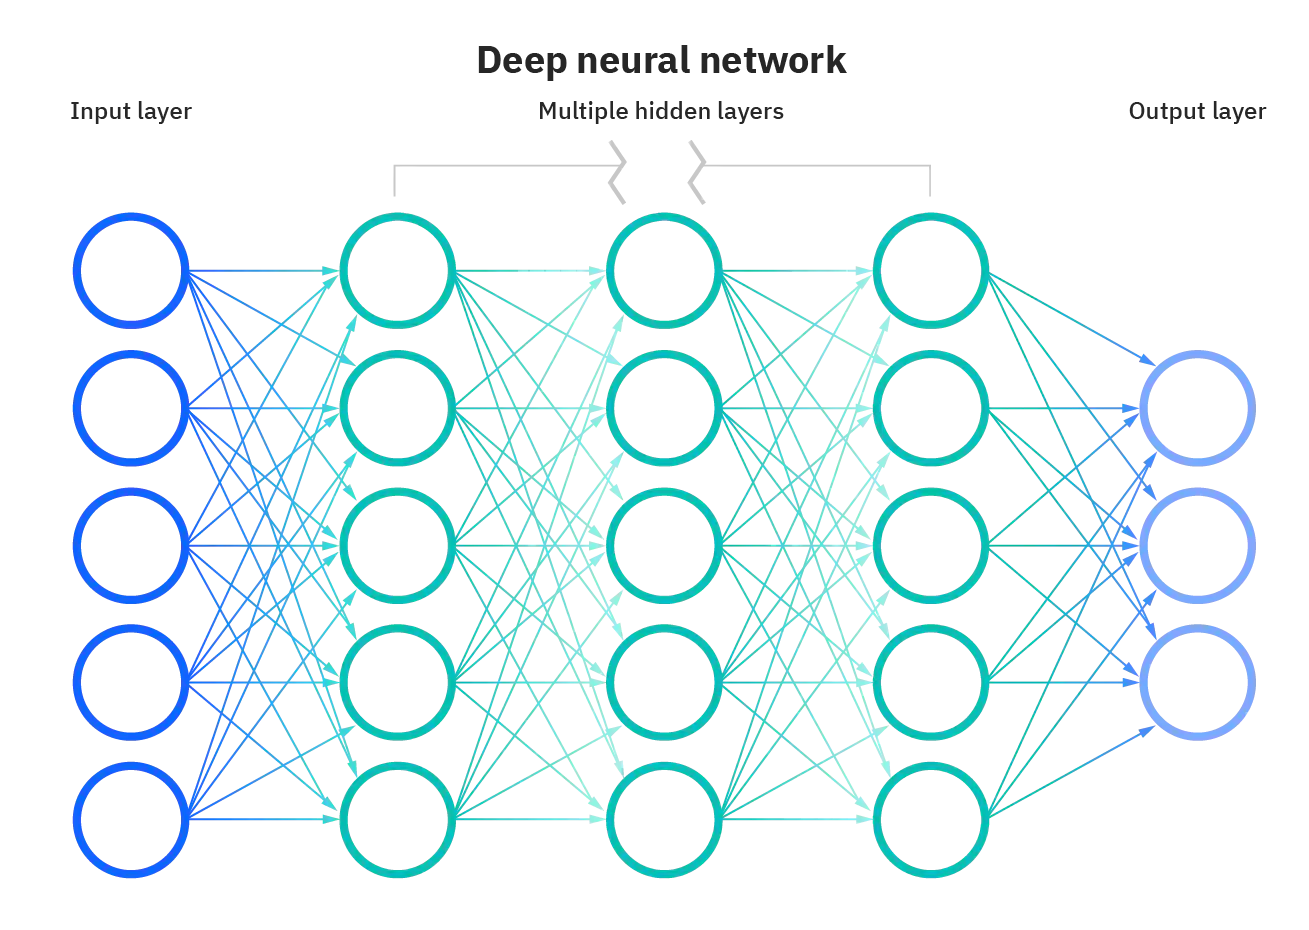
\includegraphics[width=0.45\textwidth]{figures/mlp_overview.png}
    \caption{
        A schematic overview of a feed-forward deep neural network. Source: \href{https://www.ibm.com/uk-en/cloud/learn/neural-networks}{\emph{IBM Cloud Learn Hub}}.
    }
    \label{fig:mlp_overview}
    \vspace{-12mm}
\end{wrapfigure}

\medskip
\noindent
The most simple layer used in neural networks is a linear operator:
\begin{equation*}
    L: \mathbb{R}^n \rightarrow \mathbb{R}^m , \quad L(x) = Wx + b,
\end{equation*}
parameterized by:
\begin{itemize}
    \item
        The \emph{weights matrix} $W \in \mathbb{R}^{m \times n}$, connecting input vector components (``input neurons"), to output vector components (``output neurons").
    \item
        And the \emph{biases vector} $b \in \mathbb{R}^m$ which enables unconditional shift of the output neurons
\end{itemize}
This is also known as a \emph{fully connected layer} - as each input neuron has a direct impact on each output neuron (defined by the corresponding entry in the weights matrix).

\medskip
\noindent
Recall that we defined a neural network as a concatenation of such layers - but one might notice that a concatenation of linear operators is equivalent to a single linear operator! To enable stronger representational capabilities, \emph{non-linearities} are added in-between the layers, that is - non-linear functions, known as \emph{activation functions}. Examples of popular activation functions are:
\begin{itemize}
    \item
        The sigmoid function:
        \begin{equation*}
            \sigma: \mathbb{R} \rightarrow (0,1), \quad \sigma(x) = \frac{1}{1+e^{-x}}
        \end{equation*}
    \item
        A rectified linear-unit:
        \begin{equation*}
            ReLU(x) =
                \begin{cases}
    		      0, & \text{if $x < 0$}\\
                    x, & \text{if $x \geq 0$}
                \end{cases}
        \end{equation*}
\end{itemize}
A network consisting of only fully-connected layers and non-linearities in between them is known as a \emph{fully-connected network}, a \emph{multi layer perceptron (MLP)}, or a simple \emph{feed-forward network}.

\medskip
\noindent
One activation function that's worth noting is the \emph{softmax activation}, defined over a set of neurons $x \in \mathbb{R}^n$ as follows:
\begin{equation*}
    Softmax: \mathbb{R}^n \rightarrow (0,1)^n, \quad Softmax_i(x) = \frac{e^{x_i}}{\sum_{j=1}^{n}{e^{x_j}}}
\end{equation*}
The softmax activation produces a probability distribution, as all elements in it are between 0 and 1, and they all sum up to 1. It is used in the output layer of classification networks to produce a probabilistic estimate of the input's class. The runtime values of the inputs to a softmax layer are sometimes referred to as \emph{logits}, and they quantify the un-normalized ``belief" of the network in each of the classes. A network with a single linear input layer, no hidden layers, and a single softmax output layer, is usually called a \emph{softmax classifier}, \emph{a linear classifier}, or \emph{logistic regression classifier} (although the last two may also refer to other types of classifier models).



%~~~~~~~~~~~~~~~~~~~~~~~~~~~~~~~~~~~~~~~~~~~~~~~~~~~~~~~~~~~~~~~~~
% Section 2.2: Optimization
%~~~~~~~~~~~~~~~~~~~~~~~~~~~~~~~~~~~~~~~~~~~~~~~~~~~~~~~~~~~~~~~~~

\subsection{Optimization}
\label{sec:optimization}

\subsubsection{Loss}
\label{subsec:loss}

Consider the task of estimating a certain function $f: \mathbb{R}^n \rightarrow \mathbb{R}^m$ based on a set of examples $\{x_i, y_i=f(x_i)\}_{i=1}^{N}$. Now that we've established the basics of deep learning, we may wish to approximate $f$ using a neural network - which we now know is just a long function parameterised by some set of parameters $\Theta$ defining an hypothesis function $h_\Theta: \mathbb{R}^n \rightarrow \mathbb{R}^m$. In order to ensure $h_\Theta$ approximates $f$, we can require its output on the known examples to be as close as possible to the known evaluations of $f$:
\begin{equation*}
    h_\Theta(x_i) \approx y_i = f(x_i)
\end{equation*}
But how can we formally state this requirement? One way is through a \emph{loss function} - defining the distance between the predicted output and the ground-truth for a given input:
\begin{equation*}
    \bar{\mathcal{L}}: \mathbb{R}^m \times \mathbb{R}^m \rightarrow [0,\infty)
\end{equation*}
The task can now be formulated as an optimization problem, in which we wish to find the combination of parameters $\Theta$ that minimizes the average loss of the hypothesis on all known samples:
\begin{equation}
    \min_\Theta \mathcal{L}, \quad \mathcal{L} = \frac{1}{N}\sum_{i=1}^{N}{\bar{\mathcal{L}}(h_\Theta(x_i), y_i)} \\
\end{equation}
To conclude the subsection, let's list a couple of popular loss functions used for different machine learning tasks:
\begin{itemize}
    \item
        Mean-Squared Error loss (MSE), used for regression tasks:
        \begin{equation*}
            \bar{\mathcal{L}}_{MSE}(h_\Theta(x), y) = ||h_\Theta(x) - y||^2
        \end{equation*}
    \item
        Cross-entropy loss (CE), used for classification tasks (the output of the model is assumed to be a probability distribution of classes, and the ground truth vector is assumed to be a distribution with 100\% probability for the input's actual class):
        \begin{equation*}
            \bar{\mathcal{L}}_{CE}(h_\Theta(x), y) = -\sum_{j=1}^{m}{y_j \log(h_{\Theta,j}(x))}
        \end{equation*}
        Sometimes, the exponentiation of the cross-entropy loss is used as a measure of performance - which is referred to as \emph{perplexity}.
\end{itemize}

\subsubsection{Gradient-Based Optimization}
\label{subsec:gradient}

So we wish to solve (1) - find the combinations of parameters $\Theta$ that makes $h_\Theta$ as close as possible to the ground truth $f$ on the known samples (on average). In the world of deep learning, this is usually accomplished by \emph{gradient based optimization algorithms}. Assuming that the network and the loss measure are differentiable, we can find the gradient of the error with respect to the network's parameters. This is the direction of steepest ascent of the loss, and the opposite is the direction of steepest descent of the loss. Since we wish to minimize the loss, we can construct an algorithm that iteratively steps $\Theta$ in that direction:
\begin{equation*}
    \Theta \gets \Theta - \eta \frac{\partial \mathcal{L}}{\partial \Theta}
\end{equation*}
The multiplier $\eta$ is called the \emph{learning rate}, and it controls the magnitude of the steps - the algorithm's speed and ability to perform finer updates. This iterative scheme is known as the basic \emph{gradient descent} optimization algorithm.

\medskip
\noindent
The gradient themselves are evaluated using a process known as \emph{backpropagation} - which iteratively applies the chain rule of derivation through the atomic (differentiable) calculations carried out by the various layers in the network:
\begin{equation*}
    \frac{\partial \mathcal{L}}{\partial L_i} = \frac{\partial L_{i+1}}{\partial L_i} \cdot \frac{\partial \mathcal{L}}{\partial L_{i+1}}
\end{equation*}
As the gradients are calculated from the end of the network (where the loss is directly evaluated) and propagate backwards to its beginning via the chain rule, this process is sometime referred to as a \emph{backward pass} (in contrast to the forward pass done when evaluating the network's output).

\medskip
\noindent
However, when the dataset is large, evaluating all samples in it and calculating the gradients with respects to them just to perform a single update step is way too expensive. Thus, the update steps are usually carried out using a subset of the samples each time:
\begin{equation*}
    \begin{gathered}
        B \subset \{1,...,N\}, \quad \mathcal{L}_B = \frac{1}{|B|}\sum_{i\in B}{\bar{\mathcal{L}}(h_\Theta(x_i), y_i)} \\
        \Theta \gets \Theta - \eta \frac{\partial \mathcal{L}_B}{\partial \Theta}
    \end{gathered}
\end{equation*}
These subsets of instances are usually referred to as \emph{minibatches} or just \emph{batches}. The resulting algorithm is known as the \emph{Stochastic Gradient-Descent} algorithm (SGD), as in expectation the gradient of the loss with respect to a minibatch is the same as the actual gradient of the loss with respect to the entire dataset (assuming all examples are drawn from the same source distribution). More complicated update scheme are usually Incorporated to enhance optimization - such as the ones used by the Adam optimizer (\citet{kingma2014adam}) or the momentum mechanism for SGD (\citet{qian1999momentum}).

\subsubsection{Supporting Optimization}
\label{subsec:support-optim}

Optimization by its nature is strongly affected by the behavior of the gradients. However, these tend to have an exponential behavior as feeding inputs or backpropagating gradients through linear layers has the affect of multiplication by weight matrices. These may stack up to form an unstable repeated multiplications, causing the phenomena of \emph{exploding gradients} - where gradients become exponentially large (and gradient-based optimization diverges), or \emph{vanishing gradients} - where gradients become exponentially small (and gradient-based optimization gets stuck).

\medskip
\noindent
Several methods to aid optimization and stabilize gradient flow have been developed since the recent popularization of deep neural networks. One simple approach to tackle this is to use more intelligent random initialization schemes of the model's parameters. Xavier initialization scheme (\citet{glorot2010xavier}), for instance, draws the initial weights from a specific distribution, that in theory should ensure balanced gradient flow across the network.

\medskip
\noindent
More powerful tools are \emph{normalization layers} - which normalize the output of a network's layer to have certain (learned) mean and standard deviation, ensuring stable behavior of neuron activations. A couple of popular normalization schemes are \emph{batch normalization} (\citet{ioffe2015batch}) - which normalizes the same neuron in the layer over a batch of training samples, and \emph{layer normalization} (\citet{ba2016layer}) - which normalizes all neurons in the layer over the same training sample.

\medskip
\noindent
Another very powerful technique that was first introduced by \citet{he2016deep} in their successful research \emph{``Deep residual learning for image recognition"} (\citeyear{he2016deep}) is based on \emph{residual connections}. Formally, a residual connection applied on a layer $L$ adds the layer's input to its output before continuing to the next layer:
\begin{equation*}
    L'(x) = x + L(x)
\end{equation*}
By enabling the direct propagation of information from the earlier layers to the later layers, residual connections allow the gradients to flow more efficiently through the network. This has been shown to significantly improve the overall training of neural networks, enabling stable networks with deeper architectures.


%~~~~~~~~~~~~~~~~~~~~~~~~~~~~~~~~~~~~~~~~~~~~~~~~~~~~~~~~~~~~~~~~~
% Section 2.3: Convolutional Networks
%~~~~~~~~~~~~~~~~~~~~~~~~~~~~~~~~~~~~~~~~~~~~~~~~~~~~~~~~~~~~~~~~~

\subsection{Convolutional Networks}
\label{sec:convnets}

Convolutional layers are the fundamental building block of most neural networks used for image classification and other computer vision tasks. In these layers, a set of filters or kernels are used to perform convolution operations on the input data, which essentially extracts \emph{local features} from the input image (in a linear manner). The output of a convolutional layer is a feature map that highlights important information from the input, which is then passed to the next layer for further processing. Convolutional layers play a crucial role in capturing and extracting spatial hierarchies of features from an image, allowing \emph{Convolutional Neural Networks} (ConvNets) that incorporate them to learn complex patterns and make better predictions about the contents of an image.

\begin{wrapfigure}{R}{0.45\textwidth}
    \centering
    \vspace{-2mm}
    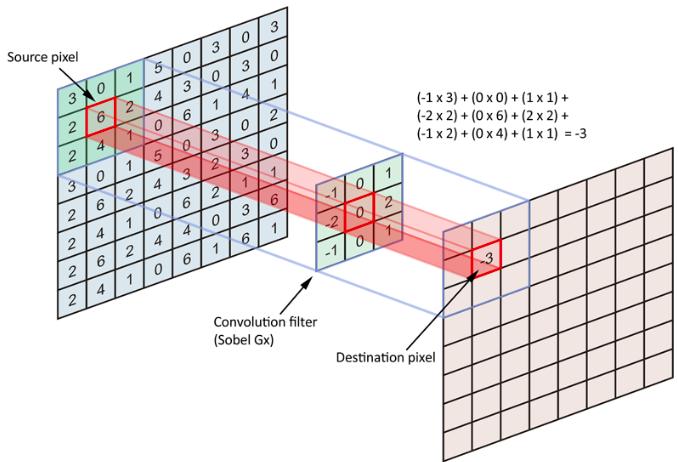
\includegraphics[width=0.4\textwidth]{figures/convolution.png}
    \caption{
        An illustration of the convolution operation. Source: \href{https://towardsdatascience.com/applied-deep-learning-part-4-convolutional-neural-networks-584bc134c1e2}{\emph{Towards Data Science}}.
    }
    \label{fig:convolution}
    \vspace{-4mm}
\end{wrapfigure}


\medskip
\noindent
Formally, the operation of a convolutional layer on an input image $I \in \mathbb{R}^{H \times W \times C}$ ($H \times W$ is the dimension of the image and $C$ is the number of channels in it) with a learned kernel $K \in \mathbb{R}^{H' \times W' \times C' \times C}$ and a learned bias vector $b \in \mathbb{R}^{C'}$ is the $C'$-channels image defined as follows:
\begin{equation*}
    (I * K)_{i,j,c'}
        = \sum_{i' = 0}^{H'-1} \sum_{j'=0}^{W'-1} \sum_{c=0}^{C-1}
            K_{i',j',c',c} \cdot  I_{i+i',j+j',c} + b_{c'}
\end{equation*}
The process is visualized in Figure \ref{fig:convolution}. This is different from a fully connected layer, in that only the $H' \times W'$ input neurons in the neighborhood of an output neuron has an effect on him, and the linear kernel weights are reused for all output neurons. This reflects the locality of the convolutional layer - locality that characterizes visual data.

\medskip
\noindent
A key feature of convolutional layer is padding, which allows the network to preserve the spatial resolution of the input data by adding zeros around the edge of the input. Stride is another feature of ConvNets, which controls the step size of the filter as it slides over the input. A larger stride results in a smaller output size. Finally, down-sampling pooling operations are often used in ConvNets to reduce the spatial resolution of the data. Max-pooling, for instance takes the maximum activation in a neighborhood of pixels, which make the network invariant to small translations in the input.

\medskip
\noindent
We'll finish our discussion by mentioning the \emph{ResNet family}. ResNet is a series of deep convolutional network architectures with integrated residual connection and increasing capacity, denoted by the number of convolutional layers they employ: ResNet-18, ResNet-34, ResNet-50 (the most popular of the five), ResNet-101 and ResNet-152. It was first presented in the same paper that originally proposed residual connections for deep networks: ``Deep Residual Learning for Image Recognition" (\citet{he2016deep}). The models in the family significantly advanced the state of the art on the ImageNet classification task and proved useful for many other applications. Even today, 8 years since they were first proposed, ResNets are still popular among the computer vision community and serve as a powerful baseline architecture for many applications.


%~~~~~~~~~~~~~~~~~~~~~~~~~~~~~~~~~~~~~~~~~~~~~~~~~~~~~~~~~~~~~~~~~
% Section 2.4: Transformers
%~~~~~~~~~~~~~~~~~~~~~~~~~~~~~~~~~~~~~~~~~~~~~~~~~~~~~~~~~~~~~~~~~

\subsection{Transformers}
\label{sec:Transformers}

\subsubsection{The Classic Transformer}
\label{subsec:Transformers}

The Transformer architecture is a type of neural network that was introduced in \citeyear{vaswani2017attention} by \citet{vaswani2017attention} in their groundbreaking paper ``Attention is All You Need". The Transformer architecture is particularly well-suited for processing sequential data, such as natural language, and has advanced the state-of-the-art on several NLP tasks. The Transformer architecture uses \emph{self-attention} mechanisms to weight the importance of different elements in the sequence and aggregate information from different parts of it to make predictions. This architecture has proven to be highly effective, allowing models to process long sequences efficiently, while maintaining the ability to capture long-range dependencies.

\medskip
\noindent
In this section, we will focus our discussion specifically on the Transformer's encoder unit, as it captures all key features behind the Transformer, and is relevant for the models later discussed in this paper. An overview of its operation is given in Figure \ref{fig:Transformer}. 

\begin{wrapfigure}{L}{0.3\textwidth}
    \centering
    \vspace{-2mm}
    \includegraphics[width=0.25\textwidth]{figures/Transformer.png}
    \caption{
        A schematic overview of the Transformer encoder unit architecture. Source: \citet{vaswani2017attention}.
    }
    \label{fig:Transformer}
    \vspace{-4mm}
\end{wrapfigure}

\medskip
\noindent
At the core of the Transformer is the \emph{self-attention mechanism}. Consider a sequence of $n$ elements $x_1,...,x_n \in \mathbb{R}^m$. Each element $x_i$ is used to generate a \emph{key} $k_i \in \mathbb{R}^{d_k}$, a \emph{query} $q_i \in \mathbb{R}^{d_k}$, and a \emph{value} $v_i \in \mathbb{R}^{d_v}$. Element $i$ attends to the value associated with element $j$ ($v_j$) based on the similarity between the query it generated ($q_i$) and the key associated with the target element ($k_j$). Softmax activation (with the logits normalized) is used to weight the $n$ value vectors element $i$ may attend to, resulting in single vector capturing the attended knowledge:
\begin{equation*}
    Attention_i(x_1,...,x_n) = Softmax(\frac{q_i^T k_1}{\sqrt{d_k}}, ..., \frac{q_i^T k_n}{\sqrt{d_k}})^T \cdot V
\end{equation*}
The layer as a whole can then be represented in matrix form as follows (where $X,K,Q,V$ are the matrices whose rows are $x_i,k_i,q_i,v_i$, respectively):
\begin{equation*}
    Attention(Q,K,V) = Softmax(\frac{QK^T}{\sqrt{d_k}})V
\end{equation*}
In practice, $Q,K,V$ are generated using simple learned linear mappings. \emph{Multiheaded self-attention} layer consists of several different instances of such attention units, whose output is concatenated together and then linearly mapped back to a lower-dimensional space (using a shared learned projection matrix), resulting in a new sequence that is passed forward to the rest of the network. Multiheaded attention is depicted in Figure \ref{fig:multi_attn}.

\medskip
\noindent
It's worth noting that for some applications, \emph{masked self-attention} must instead by employed - a mechanism in which each element can only attend to the elements that precede it in the sequence. This is carried out by discarding the key-query pairs associated with illegal combinations (where the key follows the query).

\medskip
\noindent
As depicted in Figure \ref{fig:Transformer}, the Transformer encoder is a concatenation of identical layers, each composed of 2 sub-layers:
\begin{itemize}
    \item
        Multiheaded self attention - as previously described.
    \item
        A fully connected network, which is applied to each element separately and identically. This consists of two simple linear transformations with a $ReLU$ activation in between.
\end{itemize}
Residual connections and layer-normalization are employed in-between the sub-layers to assist optimization, as discussed in subsection \ref{subsec:support-optim}.

\medskip
\noindent
You may have noticed that the Transformer block does not consider the \emph{order} of the elements in the sequence. To incorporate this information into the network's representation of the data, \emph{positional encodings} are added to the embedded representations of each element in the input sequence and helps the model understand the relative position of each element with respect to the others. One common technique for positional encoding is to add sine and cosine functions of different frequencies to the vector representations of the input elements. These functions have a unique pattern for each position in the sequence, allowing the model to differentiate between elements based on their position. By incorporating positional encoding, Transformer models proved to effectively handle sequences of varying lengths and capture the consecutive relationships between elements in a sequence.

\begin{wrapfigure}{R}{0.35\textwidth}
    \centering
    \vspace{-2mm}
    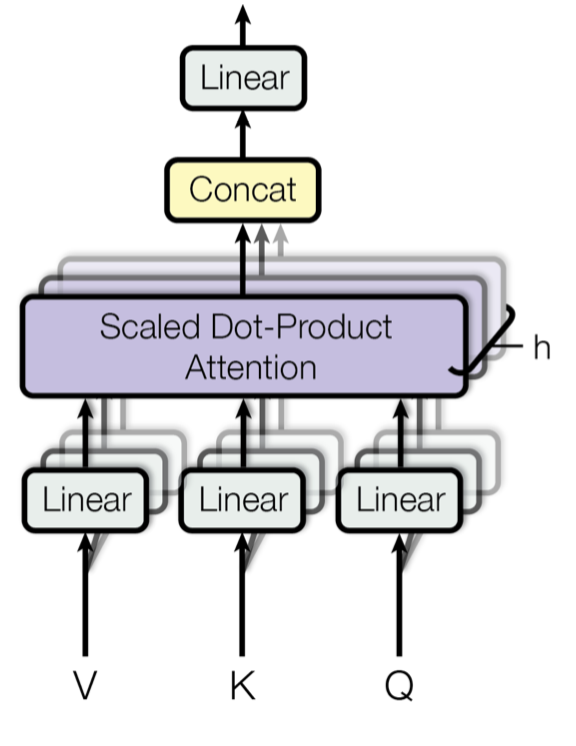
\includegraphics[width=0.3\textwidth]{figures/multi_attn.png}
    \caption{
        A schematic overview of multiheaded attention, as part of the Transformer architecture. Source: \citet{vaswani2017attention}.
    }
    \label{fig:multi_attn}
    \vspace{-8mm}
\end{wrapfigure}

\medskip
\noindent
Finally, it's worth mentioning that the dimension of the in-between vector representation of the elements in the sequence is usually kept constant across the network. This is usually referred to as the \emph{width} (or ``hidden size") of the Transformer, while the number of Transformer blocks is referred to as its \emph{depth}.


\subsubsection{Vision Transformer}
\label{subsec:vit}

Since the introduction of the Transformer in 2017, it was proved to be a powerful and scalable architecture for many natural language processing tasks. Inspired by its success, \citet{dosovitskiy2020vit} experimented with applying a standard Transformer directly to images with the fewest possible modifications, hoping to achieve similar success in computer vision. Their idea is to split the image into equally-sized patches, flatten and linearly map them onto a $d$-dimensional space using a shared (learned) projection matrix, and feed them to a Transformer as if they were just a long sequence of elements - or ``visual words". An additional learned $d$-dimensional element is added, which will carry the global representation of the image by the end of the Transformer (in a similar manner to the BERT architecture proposed by \citet{devlin2018bert}). They named the architecture \emph{Vision Transformer} (ViT).

\medskip
\noindent
\citet{dosovitskiy2020vit} experimented with various methods to adapt the positional embedding mechanism to utilize the 2-dimensional nature of the ordering of the ``elements", but came to the conclusion that when enough data is present, any sophisticated mechanism is no better than a simple mechanism based on \emph{learned positional embeddings} associated with the uniformly extracted patches in the (equally sized) training images. A Vision Transformer can thus handle images of varying resolutions, by interpolating between these learned embeddings in the 2D plane - as a varying number of patches may now be extracted.

\medskip
\noindent
The authors also provide a suite of baseline ViT architectures of varying sizes (similar to the ResNet family proposed by \citet{he2016deep}), including:
\begin{itemize}
    \item
        ViT-Base: having hidden size of 768 components, 12 layers, and 12 attention heads per layer.
    \item
        ViT-Large: having hidden size of 1024 components, 24 layers, and 16 attention heads per layer.
    \item
        ViT-Huge: having hidden size of 1280 components, 32 layers, and 16 attention heads per layer.
\end{itemize}
ViT architectures are denoted by the capacity of the corresponding Transformer, and the size of the equally-extracted patches they are fed with. For example, a ViT-L/16 refers to a ViT-Large Transformer with $16 \times 16$ input patches.



%~~~~~~~~~~~~~~~~~~~~~~~~~~~~~~~~~~~~~~~~~~~~~~~~~~~~~~~~~~~~~~~~~
% Chapter 3: GPT
%~~~~~~~~~~~~~~~~~~~~~~~~~~~~~~~~~~~~~~~~~~~~~~~~~~~~~~~~~~~~~~~~~

\newpage
\section{GPT}
\label{chap:gpt}


%~~~~~~~~~~~~~~~~~~~~~~~~~~~~~~~~~~~~~~~~~~~~~~~~~~~~~~~~~~~~~~~~~
% Section 3.1: Introduction
%~~~~~~~~~~~~~~~~~~~~~~~~~~~~~~~~~~~~~~~~~~~~~~~~~~~~~~~~~~~~~~~~~

\subsection{Introduction}
\label{sec:gpt-intro}

The first model we'll overview in this seminar, which is actually a series of models, is the \textbf{GPT} family. GPT (Generative Pre-trained Transformer) entered our lives at \citeyear{radford2018gpt1}, with the publication of the famous paper \emph{``Improving Language Understanding by Generative Pre-Training"}, by \citet{radford2018gpt1}. The paper introduced the model informally known as \emph{GPT-1} (which was not actually named yet and was simply referred to as ``Transformer LM"), that initiated a continuously-evolving fruitful research surrounding the capabilities of large-scale pre-trained Transformer-based \emph{language models} - a concept we'll thoroughly discuss in this chapter.

\medskip
\noindent
The GPT family, consisting of several powerful language models, is now known as one of the greatest Natural Language Processing systems humanity has ever possessed. As \citet{inamdar2021revolution} discusses, the astonishing abilities associated with the models in the series have revolutionized the world of Artificial Intelligence.

\medskip
\noindent
In this chapter we'll dive into the main 3 models in the GPT family - study their structure and discuss their capabilities. GPT-1 (\citet{radford2018gpt1}) - which we'll discuss in section \ref{sec:gpt1} - is in fact the least known model in the family. The more popular GPT-2 (\citet{radford2019gpt2}) was later published in 2019 and widely adopted by the research community as the team released the complete version of the the model for free by the end of 2019. We'll discuss GPT-2 in section \ref{sec:gpt2}. Finally, in section \ref{sec:gpt3} we'll overview the extensive research surrounding GPT-3 (\citet{brown2020gpt3}) - the largest and most powerful model in the series, published in 2020.

\medskip
\noindent
But first, let us begin by gathering the relevant background in Natural Language Processing and Language Modeling, so we can better understand what GPT is about.


%~~~~~~~~~~~~~~~~~~~~~~~~~~~~~~~~~~~~~~~~~~~~~~~~~~~~~~~~~~~~~~~~~
% Section 3.2: NLP: Technological Background
%~~~~~~~~~~~~~~~~~~~~~~~~~~~~~~~~~~~~~~~~~~~~~~~~~~~~~~~~~~~~~~~~~

\subsection{NLP: Technological Background}
\label{sec:nlp-background}

\subsubsection{Tokenization}
\label{subsec:tokenization}

Tokenization is a crucial step in Natural Language Processing, that involves dividing unstructured textual data into smaller meaningful units. Following \citet{webster1992tokenization}, these units are named \emph{tokens}. They are the building block of structured natural language input sequences, and are treated as individual elements in NLP tasks. They can be phrases, words, subwords, characters, or even sub-character bytes. The process of tokenization involves several important decisions, such as whether to split words based on whitespaces or punctuations, and whether to consider numbers and special characters as separate tokens. Tokenization has been extensively studied and several algorithms have been proposed for it (\citet{mielke2021between}). 

\medskip
\noindent
Let's overview the practical process of tokenization, following \citet{pai2020tokenization}. Initially, a large corpus of text is scanned and meaningful units - tokens - are extracted from it based on the \emph{tokenization algorithm}, and collected into a \emph{vocabulary}. When new text input comes - it is divided into the tokens it is composed of using the tokenization algorithm, and transformed into a mere sequence of references into the vocabulary. This structured sequence is then passed along as the input for the rest of the system.

\medskip
\noindent
Usually, special tokens are added to the vocabulary, such as the \texttt{<SOS>} (start-of-sequence) and \texttt{<EOS>} (end-of-sequence) tokens marking the boundaries of the input, the \texttt{<UNK>} token to which words not present in the vocabulary at test time may be mapped, and many others - depending on the application and tokenization algorithm.

\medskip
\noindent
Nowdays, central tokenization techniques usually involve subword segmentation algorithms, as discussed by \citet{mielke2021between}. The breakthrough for subword tokenization was the use of \emph{Byte-Pair-Encoding} (BPE; \citet{gage1994new}) by \citet{sennrich2015neural} for machine translation. To construct a vocabulary from a given text corpus, BPE starts with a poor vocabulary containing only the possible characters. It then iteratively replaces the most frequent successive pair of tokens with a new symbol representing that pair, until the vocabulary reaches a certain size. At test time, input text can be segmented in a similar manner, based on the order in which the tokens were added during training. BPE bridges the gap between character and word level language modeling: it provides the ``high-level" token representation of whole words and phrases, while preventing the need for the \texttt{<UNK>} token which models unknown lingual units ambiguously - as all possible characters are present in the vocabulary, enabling the indirect modeling of every character string.

\subsubsection{Word Embedding}
\label{subsec:embeddings}

After tokenization, natural language input is provided as a sequence of tokens - which are seemingly meaningless discrete units. \emph{Word embedding} is a technique that maps a continuous vector $e(t) \in \mathbb{R}^n$ to each token $t$ in the vocabulary, ``embedding" the token in a continuous vector space, as described by \citet{almeida2019word}.

\medskip
\noindent
These latent embeddings encapsulate the tokens' lingual meanings in a representative way that's easier for a learning model to interpret. The mapping from tokens to embeddings defines the first layer of NLP networks - the \emph{word embedding layer}, whose parameters are the embeddings themselves. These are usually learned via similar gradient-based methods in conjunction with the network itself. Word embeddings can also be transferred from open-source pre-trained systems - such as GLoVe (\citet{pennington2014glove}) or Word2Vec (\citet{mikolov2013efficient}).

\subsubsection{Language Modeling}
\label{subsec:lm}

%(if you want to cite stuff - there are examples in the comments here comments here)
% https://www.researchgate.net/profile/Mohiuddin-Qudar/publication/344158120_A_Survey_on_Language_Models/links/5f568760a6fdcc9879d62492/A-Survey-on-Language-Models.pdf
% https://web.stanford.edu/~jurafsky/slp3/3.pdf
% https://lena-voita.github.io/nlp_course/language_modeling.html
% (Fan et al., 2018) from gpt-2

\medskip
\noindent
As briefly mentioned in subsection \ref{subsec:nlp}, \emph{language modeling} is the task of assessing the likelihood of a natural language input. The goal of language modeling is to build a statistical model that can assign probabilities to sequences of tokens, such that the probability of a given sequence is a measure of the likelihood of that sequence appearing in natural language text. Language models are widely used in many NLP applications, such as speech recognition, machine translation, and text generation.

\medskip
\noindent
A language model's quality is determined by its ability to accurately predict the likelihood of sequences of words in the target language, and is usually achieved by training a learning algorithm on a (very) large corpus of text data to predict the conditional probability of a token appearing, given the history of tokens that precede it:
\begin{equation}
    P(t_n | t_{1},...,t_{n-1}) 
\end{equation}
A sequence's probability can then be evaluated using the chain rule of probabilities:
\begin{equation*}
    P(t_1,...,t_n) = \prod_{i=1}^{n} P(t_i | t_{1},...,t_{i-1})
\end{equation*}
(2) can be modeled with a probabilistic classifier, classifying sequences (such as $t_1,...,t_{n-1}$) based on the token that may follow them ($t_n$). It's worth noting that in most practical applications, due to computational constraints, a token's history is clipped to a fixed size $c$, which is usually referred to as the model's \emph{context size}. Practically, the following approximation is made:
\begin{equation*}
    P(t_n | t_{1},...,t_{n-1}) \approx P(t_n | t_{n-c},...,t_{n-1})  
\end{equation*}

\medskip
\noindent
Probably the most important application for which language models can be utilized is \emph{text generation}. Language models can generate a viable sequence of tokens one by one based on the probabilistic distribution of the next token collected from the output of the model. It is for that reason that language models are sometimes referred to as \emph{autoregressive models}, as they regress text from the same distribution of their input. There several methodologies to do so:
\begin{itemize}
    \item 
        A straightforward approach, known as \emph{greedy text generation}, iteratively appends the token that has the highest probability to follow the current generated sequence. However, this approach is prone to repetitive and unvaried outputs as it only considers a single token at each step
    \item
        \emph{Beam search} is a more sophisticated approach where the model maintains a set of the top $k$ possibilities of sequential continuations at each step, thereby generating more accurate and diverse continuations. This approach helps in avoiding repetition and improving overall quality of the generated text.
    \item
        \emph{Top-k random sampling} is yet another approach, where the model randomly samples the top k possibilities at each step, instead of only considering the highest probability outputs. This approach helps in introducing more randomness and creativity in the generated text.
\end{itemize}
The ending of a generated sequence can be indicated by the model when it generates the special token \texttt{<EOS>}.


\subsubsection{Classic NLP Tasks}
\label{subsec:nlp-tasks}

To finish our introductory background on NLP, let us overview several NLP tasks and datasets we will encounter in the remainder of the chapter.

\medskip
\noindent
\emph{Natural language inference} (sometimes referred to as \emph{NLI} or ``recognizing text entailment"), is the task of judging the logical relationship between a given pair of sentences. It's a classification task, mapping their relationship to one of three possible categories: \texttt{entailment}, \texttt{contradiction}, or \texttt{neutral}. For example:
\begin{center}
    \texttt{["At the other end of Pennsylvania Avenue, people began to line up for a White House tour.", "People formed a line at the end of Pennsylvania Avenue."] -> entailment}
\end{center}

\medskip
\noindent
\emph{Reading comprehension} (sometimes referred to as ``question answering") is a task that tests a model's ability to capture long range-dependencies and extract relevant information from large amounts of data. A sample of that task consists of 3 elements: a rather long document, a question asking about a specific thing mentioned in that document, and a set of possible answers. It's a classification task, that requires a model to assign the correct answer. \emph{RACE} (\citet{lai2017race}) is a popular dataset for this task, containing passages and associated questions collected from middle and high school exams. Another popular dataset is \emph{CoQA} (\citet{reddy2019coqa}), which integrated follow-up questions in a conversation-like manner, assessing the model's ability to rely on the historical context of a chat.

\medskip
\noindent
\emph{Commonsense reasoning} is another task that demands both single and multi-sentence reasoning. It's a classification task, that usually requires the model to select the correct choice for an omitted part of a short story. Popular datasets are: Story Cloze Test (\citet{mostafazadeh2017cloze}) - which requires the model to pick an ending to a story from 2 possible options, the Children's Book Test (CBT; \citet{hill2015cbt}) - where the objective is to identify the correct choice among 10 possible options for a word that has been omitted, and the LAMBADA dataset (\citet{paperno2016lambada}) in which the task is to anticipate the concluding word of sentences that demand a context of at least 50 tokens for a human to make an accurate prediction.

\medskip
\noindent
\emph{The Winograd Schemas Challenge} is another popular commonsense reasoning dataset, introduced by \citet{levesque2012winogrand} in \citeyear{levesque2012winogrand}, which evaluates a system's proficiency in common-sense reasoning by gauging its capacity to \emph{resolve ambiguities} in text by selecting the correct missing word in a sentence:
\begin{center}
    \texttt{"The firemen arrived after the police because they were coming from so far away. Who came from far away? [The firemen / The police]"}\\
    \texttt{Answer: "The firemen".}
\end{center}
The harder \emph{WinoGrande} challenge (\citet{winogrande}) consists of adversarially picked instances of the task - which are intentionally easier for humans than they are to machines. 

\medskip
\noindent
\emph{Semantic similarity}, also known as paraphrase detection, is a classification task that entails predicting whether two sentences have the same meaning or not. This task presents difficulties in identifying the rewording of concepts, comprehending negation, and managing syntactic ambiguity. An example is:
\begin{center}
    \texttt{"Obama speaks to the media in Illinois" <-> "The president greets the press in Chicago"}
\end{center}

\medskip
\noindent
The \emph{CoLA (Corpus of Linguistic Acceptability, \citet{warstadt2019neural}) dataset} evaluates whether a sentence is grammatically correct or not and examines the intrinsic linguistic predisposition of trained models:
\begin{center}
    \texttt{"She voted for herself." -> Correct} \\
    \texttt{"Books were sent to each other by the students." -> Wrong}
\end{center}

\medskip
\noindent
The \emph{SST-2 (Stanford Sentiment Treebank)} dataset (\citet{socher2013sst}) is a binary classification task, predicting the sentiment of a sentence (positive / negative):
\begin{center}
    \texttt{"Yet the act is still charming here" -> Positive}\\
    \texttt{"contains no wit, only labored gags" -> Negative}
\end{center}

\medskip
\noindent
The \emph{CNN and Daily Mail} dataset tests a generative model's ability to extract the relevant information from a large text, and construct sufficient summaries. It consists of large articles, and highlight paragraphs containing the most important information extracted from them.

\medskip
\noindent
To evaluate the amount of \emph{knowledge} embedded in the network's parameters, \emph{factoid-style} questions may be used, also referred to as \emph{closed book question answering}. The task usually requires the model to answer short knowledge questions such as:
\begin{center}
    \texttt{"Who wrote the book the origin of species? " -> "Charles Darwin"}
\end{center}
when provided with no context whatsoever. Various datasets have been devised for this task, including the Natural Questions dataset (\citet{kwiatkowski2019nq}), TriviaQA dataset (\citet{joshi2017triviaqa}), and WebQuestions (WebQs; \citet{webqs}).

\medskip
\noindent
Finally, the classic task of \emph{translation} from one language to another is also one of the central task in NLP, so much that a special term for this algorithmic task was coined - \emph{Machine Translation (MT)}. Success of machine translation is usually measured by the \emph{BLEU} score (bilingual evaluation understudy), described by \citet{papineni2002bleu}. Several datasets are used for this task, measuring translation capabilities between a variety of languages.


%~~~~~~~~~~~~~~~~~~~~~~~~~~~~~~~~~~~~~~~~~~~~~~~~~~~~~~~~~~~~~~~~~
% Section 3.3: GPT-1: Langauge Modeling for Fine-Tuning
%~~~~~~~~~~~~~~~~~~~~~~~~~~~~~~~~~~~~~~~~~~~~~~~~~~~~~~~~~~~~~~~~~

\subsection{GPT-1: Language Modeling for Fine-Tuning}
\label{sec:gpt1}

\subsubsection{Approach}
\label{subsec:gpt1-approach}

In this section we'll overview the first model in the GPT series, informally referred to as \emph{GPT-1} (Generative Pretrained Transformer). It was introduced in \citeyear{radford2018gpt1} in the paper \emph{``Improving Language Understanding by Generative Pre-Training"} by \citet{radford2018gpt1}.

\medskip
\noindent
The authors wished to diminish the need for large annotated datasets to solve NLP tasks using deep learning techniques. Such datasets are difficult to gather, both financially and logistically. The idea was to train a system that's able to extract linguistic and semantic information \emph{directly from large-scaled unlabeled text corpora}, that can be easily transferred to various down-stream tasks with minimal (supervised) adaptation.

\medskip
\noindent
Even when abundant supervision is accessible, unsupervised learning of powerful representations can result in substantial performance enhancements to any application, when considering the generality they offer by being trained on a diverse large-scale dataset. The widespread deployment of pretrained word embeddings in many NLP systems is a good example of that. While these methods mainly transfer word-level information, Radford et al. aimed to capture higher-level semantics of natural language input.

\medskip
\noindent
However, leveraging more than just word-level information from unannotated text raises a couple of challenges. First, what unsupervised optimization objective should we use during pretraining? And once pretraining is complete, what's the best way to transfer the learned representations to the target task?

\medskip
\noindent
As for the former challenge - \emph{language modeling objective} was chosen to learn the initial parameters of the neural network model. To fit a language model in the manner described in subsection \ref{subsec:lm}, we are only concerned with what token may follow what history of tokens. This kind of information is readily available in any text corpora, making language modeling an appealing unsupervised pretraining objective. And as for the latter challenge - once a language model is trained, its parameters can be \emph{fine-tuned} (see section \ref{sec:transfer}) to the specific target task using the relevant supervised objective.

\medskip
\noindent
Radford et al. employed a multi-layer Transformer for the language model, due to the excellent performance it has  demonstrated in the past on numerous NLP tasks. As they state, the Transformer is ideal for sequences of varying lengths, and the attention mechanism enables a more organized memory mechanism to manage long-term dependencies in text.

\medskip
\noindent
The Transformer language model works as follows: natural language input from the known corpus is fed into the Transformer. The $i$'th element of the last layer's output is then used in a probabilistic softmax classifier that compares it (by dot-product) to the original token embeddings, to predict the $i+1$'th token (see eq. (2)) . Masked attention (described in section \ref{sec:Transformers}) is employed to ensure none of the tokens ``cheat" by attending to its successors. Cross-entropy loss is used as the optimization objective for the language model:
\begin{equation*}
    \mathcal{L}_{LM} = \sum_i\log{P(t_i|t_{i-c},...,t_{i-1})}
\end{equation*}
The `Generative" part in \textbf{G}PT marks the generative nature of this approach, previously discussed in subsection \ref{subsec:lm}.

\medskip
\noindent
For training the language model, the BooksCorpus dataset (\citet{zhu2015books}) was utilized. This dataset consists of over 7,000 distinctive unpublished books from various genres, including Adventure, Fantasy, and Romance. Importantly, it comprises of extensive sequences of continuous text, enabling the generative model to learn to capture long-range dependencies.

\medskip
\noindent
Fine tuning the model for down-stream classification tasks is in fact not trivial. For tasks such as question answering or textual entailment (later discussed), the inputs may be structured in a specific way. For example, a triplet \texttt{[document, question, answer]} is a possible structure for the task of classifying whether an answer to a question is correct given a certain document in context.

\medskip
\noindent
Since the pretrained model was trained on continuous sequences of text, modifications are necessary to apply it to these structured inputs. Radford et al. employed a traversal-style approach (\citet{rocktaschel2015traversal}), where the structured inputs are converted into an ordered sequence delimited by \emph{special new tokens} (whose embeddings are randomly initialized), so it could be processed by the sequential model. These input conversions allow us to minimize changes to the architecture across tasks. Figure \ref{fig:gpt1_fig1} illustrates the process.

\begin{figure}[ht!]
    \begin{center}
        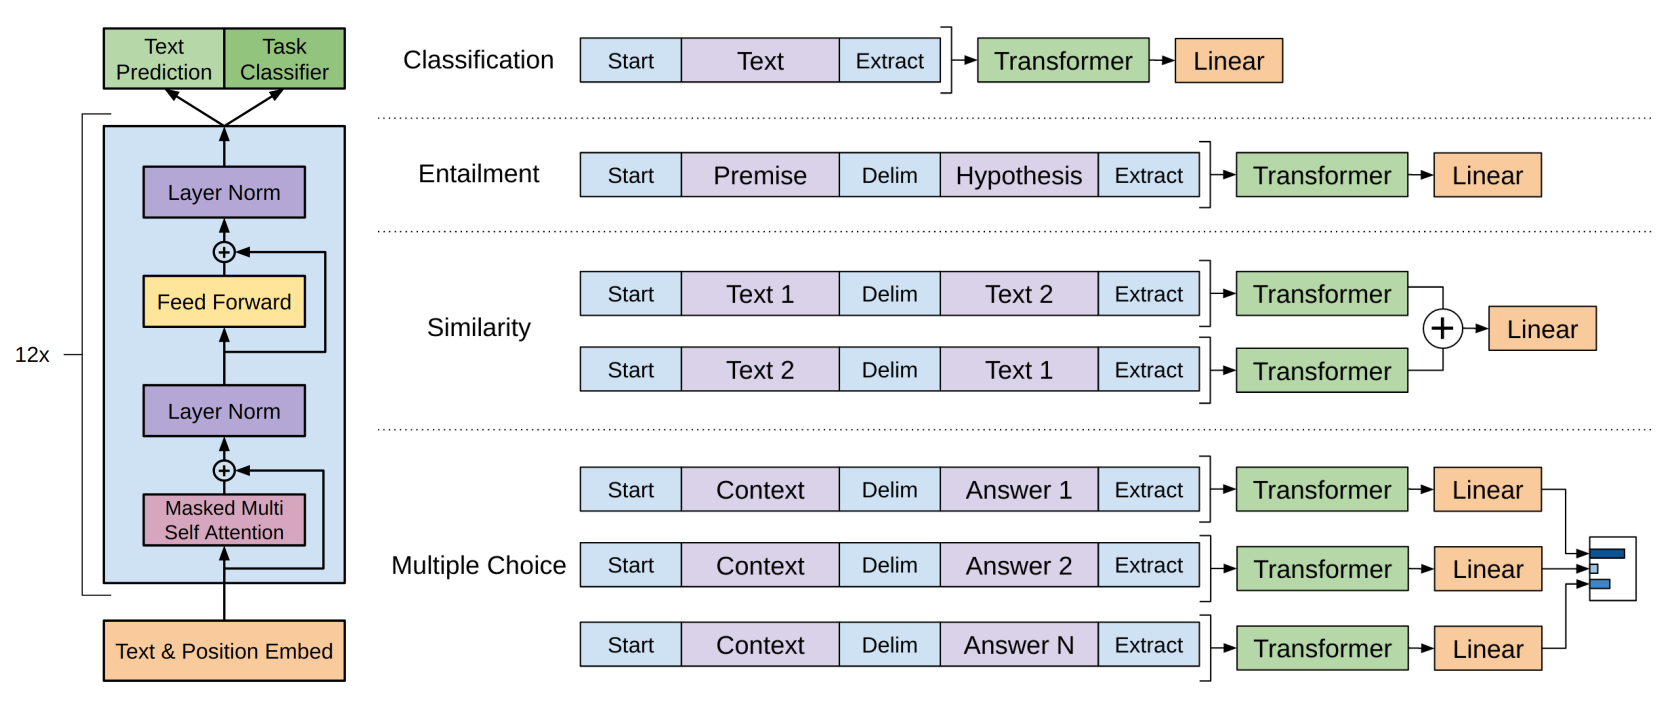
\includegraphics[clip, width=1.0\textwidth]{figures/gpt1_fig1.png}
    \end{center}
    \caption{
        Architecture and training objectives used for GPT-1 (left), and the input transformations employed for fine-tuning on different tasks (right). All inputs are converted into token sequences. Source: \citet{radford2018gpt1}.
    }
    \label{fig:gpt1_fig1}
\end{figure}

\medskip
\noindent
To classify a given sequence $x=(x_1,...,x_m)$ to a certain class $y$, the last element in the Transformer's final layer's output $h_m^{(l)}$ - associated with a new special token \texttt{<Extract>} - is then fed into a learned linear classifier:
\begin{equation*}
    P(y | x_1,...,x_m) = Softmax(W_y \cdot h_m^{(l)})
\end{equation*}
and a cross entropy loss is optimized:
\begin{equation*}
    \mathcal{L}_T=\sum_{(x,y)}\log P(y|x_1,...,x_m)
\end{equation*}
In practice, the authors discovered that incorporating language modeling as an additional objective during fine-tuning aided in learning by enhancing the generalization of the supervised model and speeding up convergence, resulting in the hybrid optimization target:
\begin{equation*}
    \mathcal{L}_H = \mathcal{L}_{LM} + \lambda \cdot \mathcal{L}_T
\end{equation*}

\medskip
\noindent
On the more technical note, it's worth mentioning some of the details of training GPT-1. A 12-layer Transformer with 12 attention heads per layer and hidden size of 768 dimensions was employed. The inner fully connected layers were 3072-dimensions wide. In total, GPT-1 had around 117M trainable parameters. For pretraining, the Adam optimizer was utilized, training for 100 epochs with batches of 64 randomly sampled sequences containing 512 tokens (and a context window of the same size). Byte Pair Encoding (BPE) was used for tokenization, on a vocabulary of around 40,000 tokens. Fine tuning was quick, and 3 epochs were mostly enough.

\subsubsection{Performance}
\label{subsec:gpt1-perform}

The research team tested the transfer capabilities of the Transformer language model they trained on a variety of classic supervised NLP tasks. In this subsection we'll overview the way the different experiments were carried out, and the performance of GPT-1 when fine-tuned for such down-stream tasks, relative to the state-of-the-art.

\medskip
\noindent
Natural language inference is tested and carried out in the sequential model by concatenating both the premise and the hypothesis, with a new special delimiter token in between. GPT-1 surpassed the current state-of-the-art baselines on four of the five datasets tested, achieving improvements of up to 5.8\% accuracy (on the QNLI dataset, introduced by \citet{wang2018glue}). This showcases the model's capacity to reason more effectively over multiple sentences and handle linguistic ambiguity.

\medskip
\noindent
For question answering, the context document and the question and concatenated to each of the possible answers. The model processes each of the resulting sequences individually and then utilizes a softmax layer to normalize the outputs, producing an output distribution over the feasible answers. Using this scheme, GPT-1 managed to outperform the previous state state-of-the-art on the RACE dataset (\citet{lai2017race}) by 5.7\% accuracy.

\medskip
\noindent
To test commonsense reasoning, a similar multi-choice framework was applied. Here, GPT-1 significantly advanced the state-of-the-art on the Story Cloze dataset \citet{mostafazadeh2017cloze} by 8.9\% accuracy.

\medskip
\noindent
Finally, for some classic classification tasks: GPT-1 managed to achieve substantial improvement of 10.4\% accuracy on the CoLA dataset (\citet{warstadt2019cola}), and was competitive with previous best-performing systems on SST-2 (\citet{socher2013sst}).


\subsubsection{Additional Analysis}
\label{subsec:gpt1-more}

In addition to evaluating GPT-1 on typical NLP challenges, the team analyzed generative pretrained Transformers from various other perspectives, to gain a deeper comprehension of their features, advantages, and limitations.

\medskip
\noindent
To test whether the model's later layers may overfit to the task of language modeling during pre-training, making them sub-optimal for down-stream tasks, Radford et al. also studied the effect of transferring a varying number of layers from unsupervised pre-training to the supervised target task. The performance of the method on the MultiNLI dataset (\citet{williams2017broad}) and RACE (\citet{lai2017race}) in relation to the number of layers transferred is presented in Figure \ref{fig:gpt1_fig2} (left). As expected, transferring embeddings enhances performance, and each Transformer layer offers additional benefits, resulting in an improvement of up to 9\% on MultiNLI when all layers are transferred. This finding suggests that each pre-trained model layer contains general valuable features for addressing any target task.

\begin{figure}[ht!]
    \begin{center}
        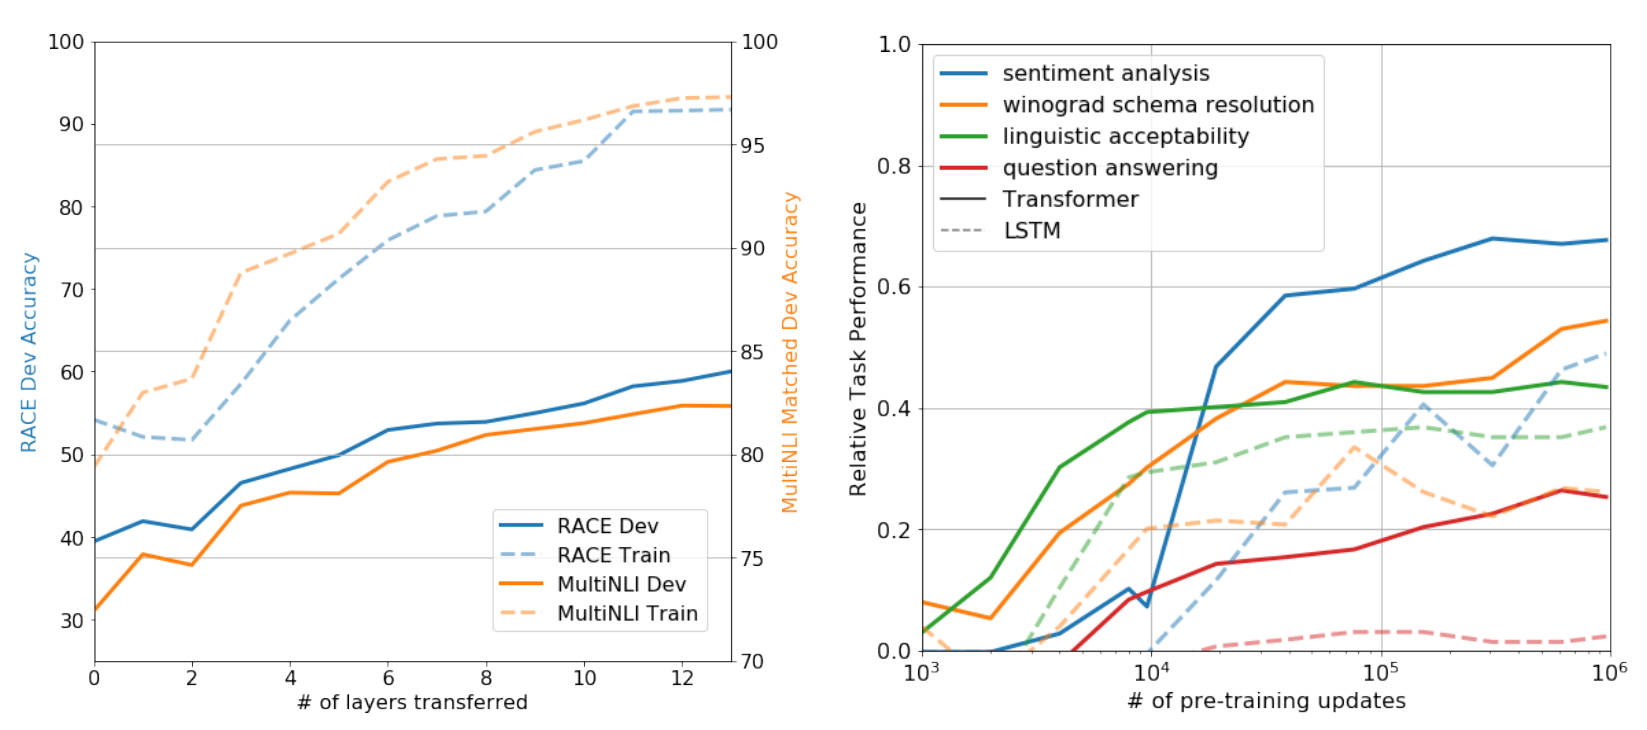
\includegraphics[width=0.8\textwidth]{figures/gpt1_fig2.png}
    \end{center}
    \caption{
        (left) Performance on RACE (\citet{lai2017race}) and MULTINLP (\citet{williams2017broad}), as a function of the number of transferred GPT-1 layers. (right) GPT-1 zero-shot performance improves through unsupervised training. Source: \citet{radford2018gpt1}.
    }
    \label{fig:gpt1_fig2}
\end{figure}

\medskip
\noindent
They also wished to understand the effect that the Transformer has on these astonishing results. They compared it with a powerful 2048-unit, single-layer LSTM (which is another neural network architecture we've not discussed, introduced by \citet{hochreiter1997lstm}). The results indicated an average score decrease of 5.6\% when the LSTM is used in place of the Transformer, hinting that the Transformer is a powerful architecture for these settings.

\medskip
\noindent
To analyze the effectiveness of pre-training on the large scale corpora prior to fitting for down-stream tasks, the team also assessed the performance of the same Transformer architecture when trained only on the relevant supervised target task, excluding pre-training. The findings demonstrate that the absence of pre-training adversely affects performance across all tasks, causing a 14.8\% average decline in accuracy in comparison to the complete model.

\medskip
\noindent
Foreshadowing OpenAI's next big research on language models, which will be shortly discussed, the authors also quickly tested the capabilities of GPT-1 when transferred to down-stream tasks with \emph{no additional supervised training} using a sequence of heuristic approaches that utilize the fundamental generative model to accomplish the tasks. Results are presented in Figure \ref{fig:gpt1_fig2} (right). It's worth noticing how the performance in these \emph{zero-shot} settings progressively improves during pre-training, indicating that language modeling facilitates the acquisition of diverse task-related features. The authors hypothesized that the underlying generative model learns to execute many of the assessed tasks to assist it with the global goal of language modeling.


%~~~~~~~~~~~~~~~~~~~~~~~~~~~~~~~~~~~~~~~~~~~~~~~~~~~~~~~~~~~~~~~~~
% Section 3.4: GPT-2: Language Modeling for Zero-Shot Transfer
%~~~~~~~~~~~~~~~~~~~~~~~~~~~~~~~~~~~~~~~~~~~~~~~~~~~~~~~~~~~~~~~~~

\subsection{GPT-2: Language Modeling for Zero-Shot Transfer}
\label{sec:gpt2}

\subsubsection{Approach}
\label{subsec:gpt2-approach}

The second model in the GPT family, now formally referred to as \emph{GPT-2}, was published in 2019 with the successful paper \emph{``Language Models are Unsupervised Multitask Learners"} by \citet{radford2019gpt2}. This research continued the line of work presented in the previous section - using a pre-trained Transformer-based language model for a diverse variety of down-stream tasks, while taking a different transferring approach. The model was very popular among the research community, as it is the most powerful language model OpenAI ever released for free.

\medskip
\noindent
The authors' main hypothesis when developing GPT-2 was that single task training on single domain datasets is a major contributor to the lack of generalization observed in current systems. Although the traditional method of training systems has been effective in making progress on narrow experts, the often erratic behavior of these models on the diversity and variety of possible inputs highlights some of the shortcomings of this approach. They mention that multitask learning (\citet{caruana1997multitask}) may be a promising framework for improving general performance, but with current approaches, it may need as much training data as for the traditional method. They conclude that exploring additional setups for performing multitask learning is necessary to improve general performance.

\medskip
\noindent
The authors follow their previous research surrounding GPT-1, which proved that language models are able perform specific tasks when there is no supervised data available (Figure \ref{fig:gpt1_fig2} (right)). To create a general system that can perform many tasks, the system should not only condition on the input (i.e. model $P(y|x)$), but also on the task to be performed (i.e. model $P(y|x,\mathcal{T})$). \citet{McCann2018multitask} demonstrate that language can be used to express tasks ($\mathcal{T}$), inputs ($x$), and outputs ($y$) altogether as sequences of symbols in a flexible manner. Language modeling has the potential to learn these tasks without explicit supervision, as the supervised objective is the same as the unsupervised objective, when only considering these subset of sequences that correspond to the relevant tasks. Thus, we may roughly state that the global minimum of the unsupervised objective is also the global minimum of the supervised objective. From this, we can draw the hypothesis that a language model with enough capacity will start to learn how to solve specific tasks presented in naturally-occurring language sequences to better predict them, even without task-specific supervision.

\medskip
\noindent
Their strategy involved gathering a vast and diverse dataset to acquire a wide range of natural language demonstrations of tasks across different domains and contexts. However, after experimentation, they opted to prioritize data quality. They achieved that by using a new web scraping method that prioritized curated and filtered web pages. To avoid high manual filtering costs, they focused on web pages that were curated by humans and had at least three karma on the social media platform \emph{Reddit} - meaning that enough users found them interesting. The resulting dataset, they named \emph{WebText}, contains the text subset of 45 million links. For training their new model, the team only used a preliminary version of WebText, that excludes links created after December 2017. The dataset contains over 8 million documents, equivalent to 40 GB of text (after de-duplication and heuristic-based cleaning).

\medskip
\noindent
The dataset is tokenized using Byte Pair Encoding, following its advantages mentioned in subsection \ref{subsec:tokenization}. It is restricted from merging across character categories for any token sequence (with the exception of the space character) to avoid many versions of the same word (for example - \texttt{"happy"}, \texttt{"happy?"}, and \texttt{"happy!"}).

\medskip
\noindent
Following its success for GPT-1, \citet{radford2019gpt2} continued to base their GPT-2 architectures on the Transformer. This time, the team trained \emph{a series} of 4 exponentially-increasing language models:
\begin{enumerate}
    \item
        With 117M parameters: a 12-layers 768-dimensions-wide Transformer (copy of GPT-1).
    \item
        With 345M parameters: a 24-layers 1024-dimensions-wide Transformer.
    \item
        With 762M parameters: a 36-layers 1280-dimensions-wide Transformer.
    \item
        With 1.54B parameters: a 48-layers 1600-dimensions-wide Transformer.
\end{enumerate}
With the latter usually referred to as \emph{GPT-2}.

\begin{wrapfigure}{R}{0.5\textwidth}
    \centering
    \vspace{-2mm}
    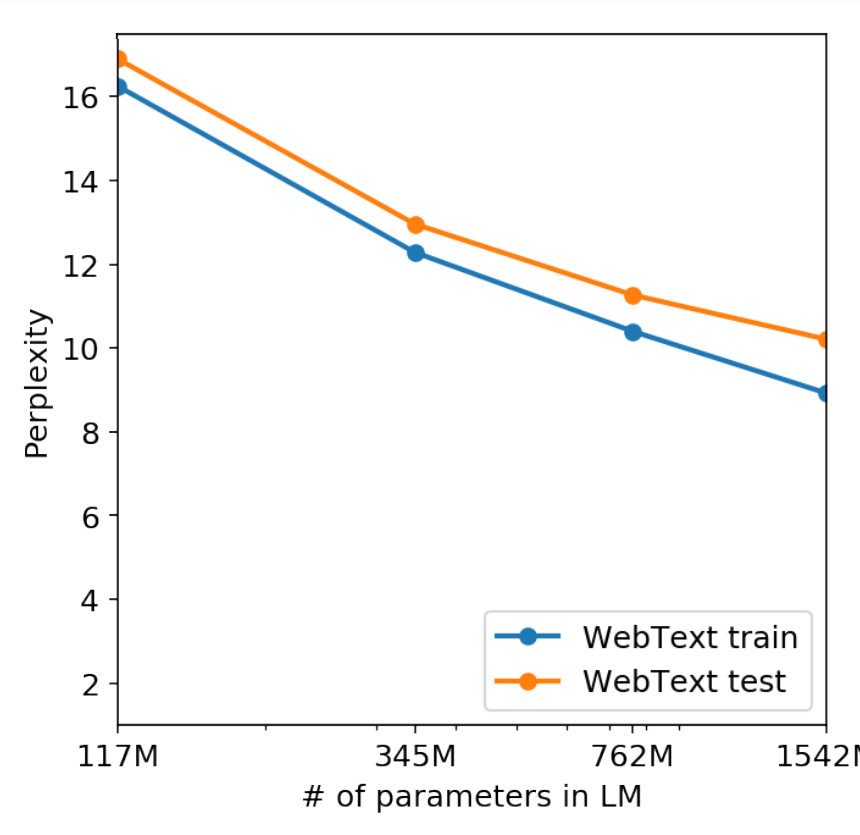
\includegraphics[width=0.45\textwidth]{figures/gpt2_fig4.png}
    \caption{
        Model size effect on GPT-2 pretraining performance. Source: \citet{radford2019gpt2}.
    }
    \label{fig:gpt2_fig4}
    \vspace{-4mm}
\end{wrapfigure}

\medskip
\noindent
Most technical details regarding the architectures and their training follow from the original GPT-1, with a few changes. Several slight modifications to the Transformer itself were applied, and a larger vocabulary of around 50,000 tokens is used, as opposed to the 40,000 tokens vocabulary of GPT-1. The context window was also expanded from 512 tokens to 1024, and training batches were enlarged from 64 samples to 512 samples each.

\medskip
\noindent
It's worth noting that as the training dataset of WebText was automatically extracted from the internet, some of the datasets on which it is evaluated down the line may accidentally overlap with it - as they are also publicly available on the web. Radford et al. were concerned with this ``data leakage", and performed an extensive analysis of the effect it may have on the model's reported performance. The analysis showed that having some shared data between the WebText training data and certain evaluation datasets may lead to slightly better reported results. However, in most cases, the overlap between standard training and test sets was already similar to the overlap between the partitions of most evaluation datasets. Figure \ref{fig:gpt2_fig4} illustrates that performance on both the training and test sets of WebText improves together as model size increases, indicating that GPT-2 is still far from overfitting the training set itself.


\subsubsection{Performance}
\label{subsec:gpt2-perform}

To test their hypothesis regarding the task-solving capabilities of mere language models, Radford et al. developed a suite of mechanisms to represent the wide variety of specific NLP tasks directly in natural language, enabling them to harness the functionality provided by the language model to develop systems that solve these tasks in a pure zero-shot manner. In this subsection we'll review the performance GPT-2 achieved in these settings on a variety of tasks.

% there are also very few graphs for specific tasks, you may consider adding them.

\medskip
\noindent
First, Radford et al. examined how well the GPT-2 models performed at zero-shot domain transfer in their primary task of language modeling. WebText LMs may face significant out-of-distribution testing for many of these datasets, as these have been aggressively pre-processed and standardized, imposing artifacts of many kinds. The results showed that WebText LMs transfer effectively to these new domains, outperforming state-of-the-art on 7 out of 8 datasets in a zero-shot setting, especially on small datasets as well as datasets that test for long-term dependencies. 

\medskip
\noindent
It is worth mentioning that in the LAMBADA language modeling dataset, the model is required to choose the best single word ending for a sentence. Investigations of GPT-2's errors revealed that while most of its predictions were valid continuations of the sentence, they were not valid final words. This indicates that the language model is not utilizing the useful constraint that the chosen word must be the final one. By adding a stop-word filter as an approximation of this constraint, the accuracy of the model increased from  52.66\% to 63.24\%, resulting in a 4\% improvement in the overall state of the art on this task.

\medskip
\noindent
With an improvement of 7\% on the Winograd Schemas Challenge, GPT-2 has achieved a new state-of-the-art accuracy of 70.70\%, which proves its ability to tackle commonsense-reasoning tasks. Moreover, GPT-2's performance is comparable to or surpasses that of three out of four baseline systems for the CoQA dataset, even without utilizing the 127,000+ question-answer pairs manually collected for training those baselines. It is impressive that GPT-2 achieves this performance without any supervised training. However, upon inspecting its answers and errors, it appears that GPT-2 frequently employs rudimentary retrieval-based heuristics, such as selecting a name from the document as the answer to a ``who" question.

\medskip
\noindent
To evaluate GPT-2's summarization capability, Radford et al. also conducted tests on the CNN and Daily Mail datasets. They prompted GPT-2 to summarize the article by appending the text "TL;DR:" and generating 100 tokens using Top-k random sampling with k = 2 to encourage more abstractive summaries and reduce repetition. They considered the first three sentences from these 100 generated tokens as the summary. Although the generated text qualitatively resembled a summary, the authors state that it often centered on recent content from the article and may include specific details. Removing the task hint reduces GPT-2's performance by 6.4 points on the aggregate metric, indicating the model's ability to \emph{exhibit task-specific behavior through natural language guidance}.

\medskip
\noindent
The researchers also tested if the language model has learned to translate between languages. To encourage GPT-2 to perform translation, they prompted the generative model for continuations of sequences of the form:
\begin{center}
    \texttt{"French: 'Je m'appelle Nadav'. English: "}\\
\end{center}
Hoping for the correct continuation:
\begin{center}
    \texttt{"'My name is Nadav'"}
\end{center}
On the WMT-14 English-French test set (\citet{bojar2014wml14}), GPT-2 achieved a BLEU score slightly worse than a word-by-word substitution. However, on the WMT-14 French-English test set, GPT-2 performed significantly better by leveraging its strong generative English model. The results surprised the researchers, as they had intentionally removed non-English webpages from the training data.

\medskip
\noindent
Finally, to evaluate the amount of knowledge embedded in the language model's learned parameters, the model was tested on the Natural Questions dataset (\citet{kwiatkowski2019nq}). Examples of question-answer pairs were included in the generative model's context to help it recognize the short-answer style of the dataset. However, even with the added guidance, the smallest model falls short of a basic baseline that returns the most frequent answer for each question type (such as \texttt{"who"}, \texttt{"what"}, and \texttt{"where"} questions). The largest LM of GPT-2 does answer 5.3 times more questions correctly, which suggests that neural system performance on this type of task is directly associated with model capacity. All in all, GPT-2 still lags behind open domain question answering systems, which use a hybrid approach of information retrieval and extractive document question answering to achieve 30-50\% accuracy.

\medskip
\noindent
As a conclusion, Radford et al. state that their findings may offer a potential explanation for why pre-training techniques have been successful in downstream NLP tasks, as we observed in the previous section when fine-tuning GPT-1. It appears that, in certain cases, these pre-training techniques are capable of learning how to perform tasks directly without requiring additional supervised adaptation or modification.

\medskip
\noindent
They still mention that despite GPT-2's ability to compete with supervised baselines, its zero-shot performance is impractical for most tasks. Even on commonly evaluated tasks, such as question answering and translation, their language models only perform better than trivial baselines when having enough capacity. Additionally, they state that there are likely many practical tasks where GPT-2's performance is still no better than random. The possibility of fine-tuning GPT-2 to down-stream tasks (similar to GPT-1) is mentioned, but left as future research direction.


%~~~~~~~~~~~~~~~~~~~~~~~~~~~~~~~~~~~~~~~~~~~~~~~~~~~~~~~~~~~~~~~~~
% Section 3.5: GPT-3: Learning at Test Time
%~~~~~~~~~~~~~~~~~~~~~~~~~~~~~~~~~~~~~~~~~~~~~~~~~~~~~~~~~~~~~~~~~

\subsection{GPT-3: Learning at Test Time}
\label{sec:gpt3}

\subsubsection{Approach}
\label{subsec:gpt3-approach}

The last model in the GPT family we'll discuss is the famous \emph{GPT-3}. GPT-3 made a huge buzz in social media, due to the outstanding capabilities this enormous model presented - hinting, for the first time ever, the possibility for true \emph{Artificial General Intelligence} (\citet{goertzel2014agi}). The research surrounding the development of the model was published in \citeyear{brown2020gpt3}, under the title ``Language Models are Few-Shot Learners", carried out by the research team of \citet{brown2020gpt3} at OpenAI. The model itself was never released to the public, and the trained parameters are considered proprietary for OpenAI.

\medskip
\noindent
Continuing GPT's line of work, the authors wished to take the idea of pretrained language models for down-stream task to the next level. The authors neglected the fine-tuning approach, arguing that fine tuning for very limited tasks distributions may lead to poor generalization. They also stated that humans - marking a possible level of achievable intelligence - can learn most language tasks without the need for huge supervised datasets, which enables them to easily switch between various tasks and skills, such as performing a math operation during a long conversation. They wished for NLP systems to also exhibit this same level of fluidity and generality.

\medskip
\noindent
In their study, they investigated the potential of using \emph{meta-learning} to tackle these challenges. Meta-learning for language models involves the acquisition of a diverse range of skills and pattern recognition abilities during the language modeling pretraining phase, which it can then leverage during the inference phase to quickly recognize and adapt to a specific task. This creates 2 phases of learning: the unsupervised pre-training step - in which gradient updates are performed to optimize the network for language modeling, and the novel \emph{in-context learning} of the fixed generative model as it reads examples of the down-stream task at test time. For example, we may quickly ``teach" the model analogies by feeding it with the following context:
\begin{center}
    \texttt{
        Find word analogies: \\
        hammer : nail :: comb : => hair \\
        white : black :: up : => down \\
        mansion : shack :: yacht : => dinghy\\}
\end{center}
And append the following line:
\begin{center}
    \texttt{light : heavy :: short : => }
\end{center}
hoping it would \emph{learn} from the first three examples that it needs to generate the correct continuation: \texttt{long}. The novelty is this approach lies in the fact that \emph{no gradient updates} are performed during in-context learning - as Figure \ref{fig:gpt3_fig2_1} depicts. Inference must directly be carried out by the parameters of the network. A pretrained model that's able to learn at test time is the authors' ``vision" behind GPT-3.

\begin{figure}[ht!]
    \begin{center}
        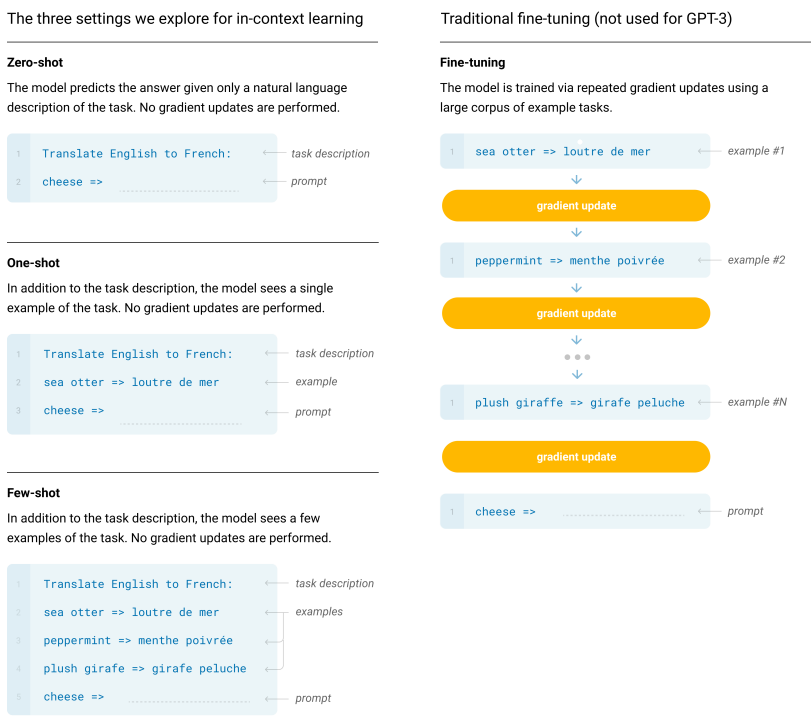
\includegraphics[width=1.0\textwidth]{figures/gpt3_fig2_1.png}
    \end{center}
    \caption{
        (left) In-context learning: the transfer methodologies behind GPT-3. (right) Traditional transfer through fine-tuning. Source: \citet{brown2020gpt3}.
    }
    \label{fig:gpt3_fig2_1}
\end{figure}

\medskip
\noindent
As the series of GPT-2 architectures proved (Figure \ref{fig:gpt2_fig4}), increasing the model's size leads to a smooth improvement in log loss, which is a good indicator for downstream tasks. As in-context learning encompasses many skills and tasks within the model's parameters, it's possible that it too will improve with larger models. Brown et al. takes this hypothesis to the extreme, training a series of 8 models with increasing size, the largest of which reaching the unbelievable magnitude of 175.0B parameters. Table \ref{tab:gpt3_tab2_1} summarizes the GPT-3 series of Transformer architectures (also note the increased batch size used for training, as opposed to the 512-sized batch of GPT-2 or the 64-sized batch of GPT-1).

\medskip
\noindent
They evaluated GPT-3 for each task under three conditions:
\begin{itemize}
    \item
        ``Few-shot learning" or in-context learning, where the model is given a few task demonstrations at inference time as conditioning, but no weight updates are allowed.
    \item
        ``One-shot learning" where the model is allowed only one demonstration in addition to natural language task description, which closely matches how some tasks are communicated to humans.
    \item
        ``Zero-shot learning" where no demonstrations are allowed, and the model is only given a natural language instruction describing the task. This is the most challenging setting and is closest to how humans perform tasks in most cases.
\end{itemize}

\noindent
To evaluate few-shot learning, the authors use a process that involves randomly selecting K examples from a task's training set as conditioning, separated by 1 or 2 newlines (depending on the task). They mention that the value of K was usually better when larger, and was selected by testing the model on validation sets. For tasks that require selecting one correct completion from multiple options, they provide K examples of context plus correct completion, followed by one example of context only. Then they compare the likelihood of each completion using the language model probability estimations. For tasks that involve binary classification, they decided to assign more semantically meaningful names, such as \texttt{"True"} or \texttt{"False"}, instead of \texttt{0} or \texttt{1}, and treat the task as a multiple-choice question. For tasks with free-form completion, they utilize beam search for text generation.

\begin{table}[ht!]
    \begin{center}
        \begin{tabular}{c c c c c c}
            \hline
            \addlinespace
            Model Name & $n_{\texttt{params}}$ & $n_{\texttt{layers}}$ & $d_{\texttt{model}}$ & $n_{\texttt{heads}}$ & Batch Size \\
            \addlinespace
            \hline
            \addlinespace
            GPT-3 Small & 125M & 12 & 768 & 12 & 0.5M \\
            GPT-3 Medium & 350M & 24 & 1024 & 16 & 0.5M \\
            GPT-3 Large & 760M & 24 & 1536 & 16 & 0.5M \\
            GPT-3 XL & 1.3B & 24 & 2048 & 24 & 1M \\
            GPT-3 2.7B & 2.7B & 32 &2560 &32 & 1M \\
            GPT-3 6.7B & 6.7B & 32 & 4096 & 32 & 2M \\
            GPT-3 13B & 13.0B & 40 & 5140 & 40 & 2M \\
            GPT-3 175B or ``GPT-3" & 175.0B & 96 & 12288 & 96 & 3.2M \\
            \addlinespace
            \hline
        \end{tabular}
        \caption{
            Specifications of the models in the GPT-3 series. Source: \citet{brown2020gpt3}.
        }
        \label{tab:gpt3_tab2_1}
        \vspace{-6mm}
    \end{center}
\end{table}

\medskip
\noindent
The technical methodologies for training GPT-3 are similar to GPT-2, with increased model sizes, longer training, larger dataset (described in the next subsection), and slight modifications to the underlying Transformer architecture. The same BPE tokenizer used for GPT-2 is reused for GPT-3.


\subsubsection{Dataset}
\label{subsec:gpt3-dataset}

Brown et al. based their training dataset for GPT-3 on the \emph{Common Crawl archive}. Common Crawl is an extensive web data repository that provides free and open access to web pages and associated metadata. It employs a web crawler to collect the data, which starts with a seed set of URLs and recursively follows links to discover new web pages. The crawler collects every website it encounters. Once collected, the data is processed, cleaned, compressed and added to the Common Crawl archive.

\medskip
\noindent
The training dataset included some of Common Crawl's partitions, covering 2016 to 2019, which amounted to 45TB of compressed plain text before filtering and 570GB after filtering, or approximately 400 billion tokens. Brown et al. found that Common Crawl's unfiltered or lightly filtered versions had lower quality compared to more curated datasets. To improve the average quality of the data, they included additional high-quality reference corpora in the training mix. During training, those datasets were sampled more frequently, accepting a small amount of overfitting in exchange for better quality of data.


\subsubsection{Performance}
\label{subsec:gpt3-perform}

Like GPT-2, GPT-3 was first tested on the task of language modeling. In the zero shot settings it achieved 76\% accuracy on LAMBADA (\citet{paperno2016lambada}) - around \%8 better than the previous SOTA, while reaching new heights with 86.4\% when utilizing few-shot-in-context learning. GPT-3 also performs at 83.2\% in the zero-shot setting and 87.7\% in the few-shot setting (using 70 examples in context) when tested on the StoryCloze dataset (\citet{mostafazadeh2017cloze}). Despite being 4.1\% lower than state-of-the-art systems that have been fine-tuned, these results still represent an improvement of approximately 10\% compared to previous zero-shot outcomes.

\medskip
\noindent
To test the factual knowledge the model absorbed in its parameters during pre-training, GPT-3 is also tested for closed-book question answering. The one-shot performance of GPT-3 on TriviaQA (\citet{joshi2017triviaqa}) matches that of a SOTA open-domain QA system, which employs both fine-tuning and a learned retrieval mechanism (\citet{retrieval}). It achieves another 3.2\% in few-shot. On both WebQs (\citet{webqs}) and Natural Questions (\citet{kwiatkowski2019nq}) there is a significant improvement from zero-shot to few-shot. This suggests that the format of the samples in these sets might be different from what GPT-3 is used to, although it successfully adapts to it in few-shot. On WebQs the few-shot system approaches SOTA, while it is less competitive for the Natural Questions fine-grained knowledge dataset. There is also a smooth trend of improvement with model capacity - suggesting that the size of the model is directly associated with absorbed knowledge.

\medskip
\noindent
\citet{brown2020gpt3} mention that although GPT-3's zero-shot Machine Translation capabilities were impressive, it still underperforms some of the more recent unsupervised systems. They also note that there is a noticeable imbalance in translation ability between different language directions. Specifically, GPT-3 performs much better when translating into English than when translating from English.

\medskip
\noindent
To test its common-sense reasoning skills, GPT-3's performance on the Winogrand Schema Challenge (\citet{levesque2012winogrand}) was measured. Its zero-shot, one-shot, and few-shot settings achieved strong results of 88.3\%, 89.7\%, and 88.6\%, respectively, without clear evidence of in-context learning. Although these results are slightly below state-of-the-art, they are still impressive. On the more challenging WinoGrande dataset (\citet{winogrande}), GPT-3's in-context learning led to some improvement, but it underperformed relative to the state-of-the-art.

\medskip
\noindent
GPT-3's reading comprehension ability was evaluated on 5 different datasets that use abstractive, multiple choice, and span-based answer formats in both dialog and single question settings. The results show a wide variation in GPT-3's performance across these datasets, which suggests that it has varying capabilities with different answer formats. Overall, the authors state that GPT-3's performance is comparable to initial baselines and early results for this NLP task.

\medskip
\noindent
GPT-3's natural language inference ability was also evaluated using the RTE dataset (\citet{rte1}) and the adversarially mined ANLI dataset (\citet{anli}). Only the largest version of GPT-3 performed better than random on both datasets, but still insufficiently. Overall, the authors mention that GPT-3 seems to struggle in tasks involving the comparison of two sentences or snippets.

\medskip
\noindent
GPT-3 was evaluated in the few-shot or zero- and one-shot setting using various tasks to test its ability to perform on-the-fly computational reasoning, recognize novel patterns, and adapt to unusual tasks. It performed well on simple arithmetic problems in natural language, with performance decreasing as the number of digits increases. GPT-3 was also able to learn novel symbolic manipulations from a few examples and can recognize and use nonexistent words it's taught in its context. Additionally, it managed to generate synthetic news articles that were difficult for humans to distinguish from human-written ones. However, it still struggled with correcting English grammar and understanding the contextual nuances of language. 


\subsubsection{Additional remarks}
\label{subsec:gpt3-more}

In this final subsection we cover a few more remarks and observations Brown et al. raised during their extensive research developing the powerful GPT-3 model.

\begin{wrapfigure}{R}{0.6\textwidth}
    \centering
    \vspace{-2mm}
    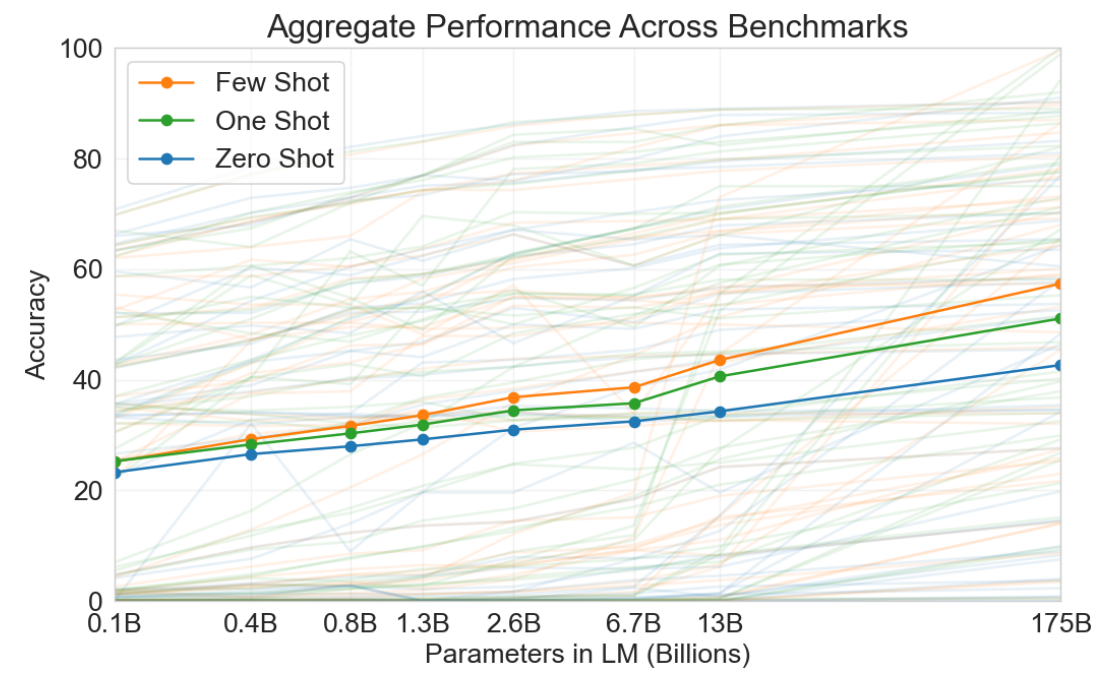
\includegraphics[width=0.55\textwidth]{figures/gpt3_fig1_3.png}
    \caption{
        Effect of model size and in-context transfer methodology on GPT-3 average performance. Lighter lines represent performance on specific benchmarks, which tends to be rather noisy. Source: \citet{brown2020gpt3}.
    }
    \label{fig:gpt3_fig1_3}
    \vspace{0mm}
\end{wrapfigure}

\medskip
\noindent
It's worth comparing the different settings to each other, to learn more about the significance of the different parts in play. First, through all tasks, performance tends to smoothly improve with the increasing size of the model. This is summarized in Figure \ref{fig:gpt3_fig1_3}. Moreover, it also seems like the number of examples provided in context for few-shot learning has a direct effect on performance too, as Figure \ref{fig:gpt3_fig1_2} depicts.

\medskip
\noindent
Although it has made remarkable progress in the field of natural language processing, Brown et al. mention that GPT-3 still faces several limitations. One of the main drawbacks is related to text synthesis, where the overall quality is high but GPT-3 samples still exhibit semantic repetition at the document level, loss of coherence over long passages, contradictions, and non-sequitur sentences or paragraphs. Additionally, GPT-3 has difficulty with ``common sense physics", performs poorly on some ``comparison" tasks, and struggles with reading comprehension in some cases.

\medskip
\noindent
Another limitation of GPT-3 the authors bring to our attention is that the current objective weights every token equally, lacking a notion of what is more important to predict. Moreover, large pretrained language models are not grounded in other domains of experience, such as video or real-world physical interaction, and therefore lack a lot of context about the world. They also mention that the model sees more text during pre-training than a human sees in their lifetime, which raises ambiguity about whether few-shot learning actually learns new tasks ``from scratch" at inference time - like humans - or simply recognizes and identifies tasks it has learned during training.


\begin{wrapfigure}{L}{0.6\textwidth}
    \centering
    \vspace{-2mm}
    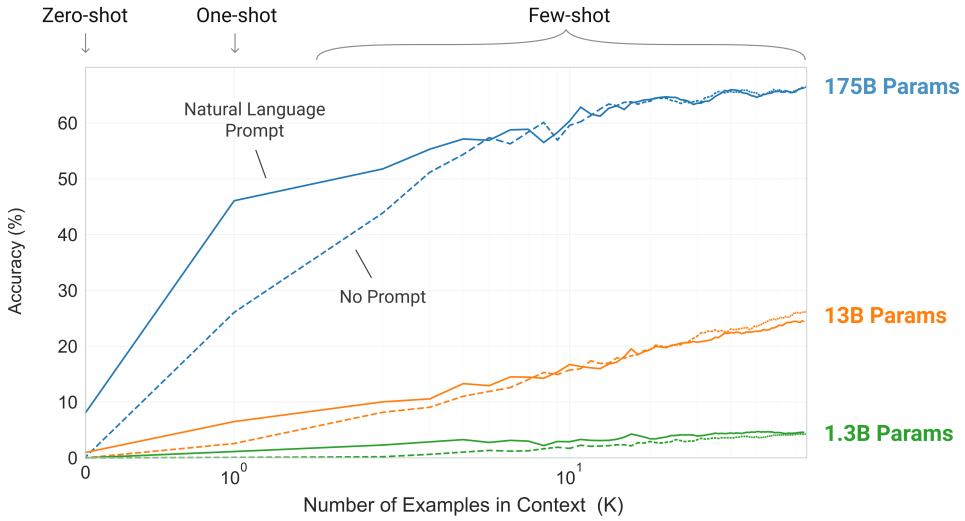
\includegraphics[width=0.55\textwidth]{figures/gpt3_fig1_2.png}
    \caption{
        GPT-3 performance improves with the number of examples in its context: the model learns at test time. Source: \citet{brown2020gpt3}.
    }
    \label{fig:gpt3_fig1_2}
    \vspace{-2mm}
\end{wrapfigure}

\medskip
\noindent
Finally, the authors also emphasize that as with most deep learning systems, the decisions GPT-3 makes are not easily interpretable, not well-calibrated in their predictions, and retain biases from the data they have been trained on.

\medskip
\noindent
As a final remark, one promising direction mentioned towards the ending the paper is learning the objective function directly from human instructors through \emph{reinforcement learning techniques}. By doing so, it may be possible to address some of the limitations of GPT-3 and improve its overall performance. A follow-up paper by \citet{ouyang2022training} investigates this approach, and introduces the \emph{InstructGPT} model -  which forms the basis for the famous chat platform of OpenAI, known as \emph{ChatGPT}. Unfortunately, these are beyond the scope of this seminar.



%~~~~~~~~~~~~~~~~~~~~~~~~~~~~~~~~~~~~~~~~~~~~~~~~~~~~~~~~~~~~~~~~~
% Chapter 4: CLIP
%~~~~~~~~~~~~~~~~~~~~~~~~~~~~~~~~~~~~~~~~~~~~~~~~~~~~~~~~~~~~~~~~~

\newpage
\section{CLIP}
\label{chap:clip}


%~~~~~~~~~~~~~~~~~~~~~~~~~~~~~~~~~~~~~~~~~~~~~~~~~~~~~~~~~~~~~~~~~
% Section 4.1: Introduction
%~~~~~~~~~~~~~~~~~~~~~~~~~~~~~~~~~~~~~~~~~~~~~~~~~~~~~~~~~~~~~~~~~

\subsection{Introduction}
\label{sec:clip-intro}

The second model we'll overview in this seminar is \textbf{CLIP} (Contrastive Language-Image Pre-training). CLIP was introduced in February 2021 by a group of researchers at OpenAI, in their highly quoted paper \emph{Learning Transferable Visual Models From Natural Language Supervision}, by \citet{radford2021clip}. As we will see, CLIP is an extremely powerful and flexible tool, connecting visual concepts with natural language. The trained models were publicly published by the team - providing researchers and practitioners all around the world with the ability to develop their own applications on top of it.

\medskip
\noindent
In section \ref{sec:clip-approach} we'll study the unique suite of concepts upon which the development of CLIP was based. In section \ref{sec:clip-training} we'll overview the models that surround CLIP, and the process of their training. In section \ref{sec:clip-transfer} we'll explore CLIP's strengths and weaknesses through transfer to a wide variety of classification tasks. Finally, in section \ref{subsec:clip-multimodal} we'll gain a deeper understanding of CLIP by looking at astonishing patterns that appear when examining the activations of the neurons in the trained model.


%~~~~~~~~~~~~~~~~~~~~~~~~~~~~~~~~~~~~~~~~~~~~~~~~~~~~~~~~~~~~~~~~~
% Section 4.2: Approach
%~~~~~~~~~~~~~~~~~~~~~~~~~~~~~~~~~~~~~~~~~~~~~~~~~~~~~~~~~~~~~~~~~

\subsection{Approach}
\label{sec:clip-approach}

\citet{radford2021clip} were encouraged by the success of pre-training models directly from raw text for NLP tasks using large collections of web text portrayed by the GPT family, and sought to explore how scalable pre-training methods that learn directly from web text could lead to a similar breakthrough in the field of computer vision. 

\medskip
\noindent
They considered the possibility of using natural language to connect imagery with a broad range of visual concepts. They emphasized the value of natural language as a training signal and its ability to express an unlimited set of visual concepts through its generality. They also appreciated the scalability of this approach - as it enables models to learn passively from the vast amounts of text available on the internet. Furthermore, they point out that using natural language supervision not only enables the learning of general image representations, but also connects those representations to language - a powerful tool for representing almost every possible concept, which may enable flexible language-based zero-shot transfer methodologies.further down the line.

\medskip
\noindent
The concept of connecting imagery and language has been around for ac couple of decades, as seen in earlier papers such as \citet{mori1999image}. However, the performance of these approaches was limited. They often relied on primitive representations such as bags-of-words (\citet{joulin2016learning}) or n-grams (\citet{li2017learning}). Others were based on varying-quality datasets (such as the YFCC100M dataset by \citet{thomee2016yfcc100m}, were too application specific (such as the work of \citet{zhang2022contrastive} for medical imaging), or used small datasets in comparison to modern computer vision datasets (such as the MS COCO dataset by \citet{lin2014mscoco}). In contrast, successful approaches in NLP relied on very large scale training. The authors aim to close this performance gap by exploring a new approach to learn visual representations directly from large-scale internet-based datasets. 

\medskip
\noindent
In order to achieve their objective, the researchers created a new dataset, named WIT (WebImageText), consisting of 400 million pairs of images and text. WIT was constructed by collecting a large number of image and text pairs from various publicly available sources on the internet using web-crawling techniques. The dataset was balanced across multiple variables, such as object types and image quality, and covers a broad range of visual concepts. The images were obtained from public image-sharing platforms, such as Flickr and Instagram, and were filtered to remove duplicates and low-quality images. The text was obtained from associated metadata, such as image captions and tags, as well as surrounding textual content, such as article headlines and social media posts. The WIT dataset was designed to be diverse and representative of the full range of visual concepts, with unsupervised and supervised methods used for data collection and filtering.
 
\medskip
\noindent
The authors of the CLIP model found that predicting captions, as previously done in the VirTex architecture (\citet{desai2021virtex}), was suboptimal. Instead, they improved the model's performance by exploring the use of a \emph{contrastive objective}, as described in previous work by \citet{zhang2022contrastive} in the field of medical imaging. Specifically, Given a batch of $N$ $(image, text)$ pairs:
\begin{equation*}
    (I_1,T_1),...,(I_n,T_n) \in \mathcal{I} \times \mathcal{T}
\end{equation*}
CLIP is trained to predict which (image, text) pairs actually occurred by jointly training an image encoder and text encoder:
\begin{equation*}
    ImageEncoder: \mathcal{I} \rightarrow \mathbb{R}^d, \quad 
    TestEncoder: \mathcal{T} \rightarrow \mathbb{R}^d
\end{equation*}
to maximize the cosine similarity of the embeddings of the $n$ real pairs in the batch while minimizing the cosine similarity of the embeddings of the $n^2-n$ incorrect pairings:
\begin{equation*}
    \begin{gathered}
         logits =e^{\tau} \times  CosineSimilarity(ImageEncoder(I_1,...,I_n), TextEncoder(T_1,...,T_n)) \\
         (logits \in \mathbb{R}^{n \times n})
    \end{gathered}
\end{equation*}
(with a learned temperature parameter $\tau$), and optimize a symmetric cross-entropy loss (\citet{wang2019symmetric}) over these similarity scores:
\begin{equation*}
    \mathcal{L}_{SCE} = \mathcal{L}_{CE}(Softmax(logits)) + \mathcal{L}_{CE}(Softmax(logits^T))
\end{equation*}


%~~~~~~~~~~~~~~~~~~~~~~~~~~~~~~~~~~~~~~~~~~~~~~~~~~~~~~~~~~~~~~~~~
% Section 4.3: Models and Training
%~~~~~~~~~~~~~~~~~~~~~~~~~~~~~~~~~~~~~~~~~~~~~~~~~~~~~~~~~~~~~~~~~

\subsection{Models and Training}
\label{sec:clip-training}

Two different architectures are utilized for the vision encoders in the different CLIP models:
\begin{itemize}
    \item 
        A set of ResNets with varying scale, including ResNet-50 and ResNet-101, as well as three additional models denoted as RN50x4, RN50x16, and RN50x64, respectively. These models follow the EfficientNet-style scaling approach (\citet{tan2019efficientnet}) and use about 4x, 16x, and 64x the compute of ResNet-50, with a few slight modifications to the original ResNet architecture.
    \item
        Vision Transformers, which include a ViT-B/32, a ViT-B/16, and a ViT-L/14. To further enhance the performance of the ViT-L/14 model, it is also pre-trained at a higher image resolution of 336 pixels (and subsequently denoted ViT-L/14@336px), similar to the approach of FixRes (\citet{touvron2019fixing}). The latter model is the one usually associated with the name \emph{CLIP} (unless otherwise stated), which the authors found to perform best.
\end{itemize}

\medskip
\noindent
The text encoder used in CLIP is a variant of the GPT-2 Transformer architecture (\citet{radford2019gpt2}). The base model is a 12-layer, 63M-parameter model with a width of 512 and 8 attention heads. The text is tokenized using byte pair encoding (BPE) with a vocabulary size of 49,152 (Sennrich et al., 2015), and is capped at a maximum sequence length of 76 for computational efficiency. The width of the text encoder is scaled proportionally to the increase in width of the ResNet, but the depth is not scaled, as the researchers found that CLIP's performance was not very sensitive to the capacity of the text encoder. The input sequence is prepended with the start-of-sequence \texttt{[SOS]} token and appended with the end-of-sequence \texttt{[EOS]} token, and the output vector of the highest layer of the Transformer at the \texttt{[EOS]} token is used as the feature representation vector of the text. 

\medskip
\noindent
Finally, the representation vectors extracted from both vision and text encoders are linearly mapped using learned projection matrices to a joint embedding space - where they are compared against one another.

\medskip
\noindent
Quickly delving into the technical details, we mention that CLIP is trained from scratch using a minibatch size of 32,768 and the Adam optimizer (\citet{kingma2014adam}). Additionally, as previously mentioned, the temperature parameter which controls the range of the logits in the softmax, $\tau$, is directly optimized as well. Various other techniques were utilized to support the training process. The largest ResNet model, RN50x64, required 18 days of training on 592 V100 GPUs, while the largest Vision Transformer took 12 days on 256 V100 GPUs. The training process altogether took 30 days across 592 V100 GPUs. It's noteworthy that training these models on AWS on-demand instances would have cost a staggering \$1,000,000! (\citet{expensiveclip}).

%~~~~~~~~~~~~~~~~~~~~~~~~~~~~~~~~~~~~~~~~~~~~~~~~~~~~~~~~~~~~~~~~~
% Section 4.4: Transfer Capabilities
%~~~~~~~~~~~~~~~~~~~~~~~~~~~~~~~~~~~~~~~~~~~~~~~~~~~~~~~~~~~~~~~~~

\subsection{Transfer Capabilities}
\label{sec:clip-transfer}

\citet{radford2021clip} used the term ``zero-shot learning" to evaluate a machine learning system's ability to learn and generalize to unseen tasks and datasets. They wished to analyze the abilities CLIP achieved during pre training - similar to how GPT-2 and GPT-3 have demonstrated when applied to downstream tasks with no additional tuning.

\medskip
\noindent
In this section we explore the capabilities and limitations of CLIP - as a zero-shot end-to-end classifier, and as an extractor of transferable feature vectors for visual data, testing its task-learning capabilities and robustness to distribution shifts.


%~~~~~~~~~~~~~~~~~~~~~~~~~~~~~~~~~~~~~~~~~~~~~~~~~~~~~~~~~~~~~~~~~
% Sub Section 4.4.1: Zero-Shot Transfer Methodologies
%~~~~~~~~~~~~~~~~~~~~~~~~~~~~~~~~~~~~~~~~~~~~~~~~~~~~~~~~~~~~~~~~~

\subsubsection{Zero-Shot Transfer Methodologies}
\label{subsec:clip-zs-methods}

The computer vision task discussed by \citet{radford2021clip} are \emph{classification tasks} - in which a system is required to predict the correct class to which the contents of an image belong. For example - classify whether an image contains a dog or rather a cat. The novelty in the approach of CLIP is that its multi-modal embedding space associates imagery with \emph{natural language} - which can be utilized to express any visual concepts associated with any class. For example, An image's encoding can be compared against the encodings of the prompts \texttt{"dog"} and \texttt{"cat"} and accordingly classified with \emph{no additional task-specific training}.

\begin{wrapfigure}{L}{0.5\textwidth}
    \centering
    \vspace{-2mm}
    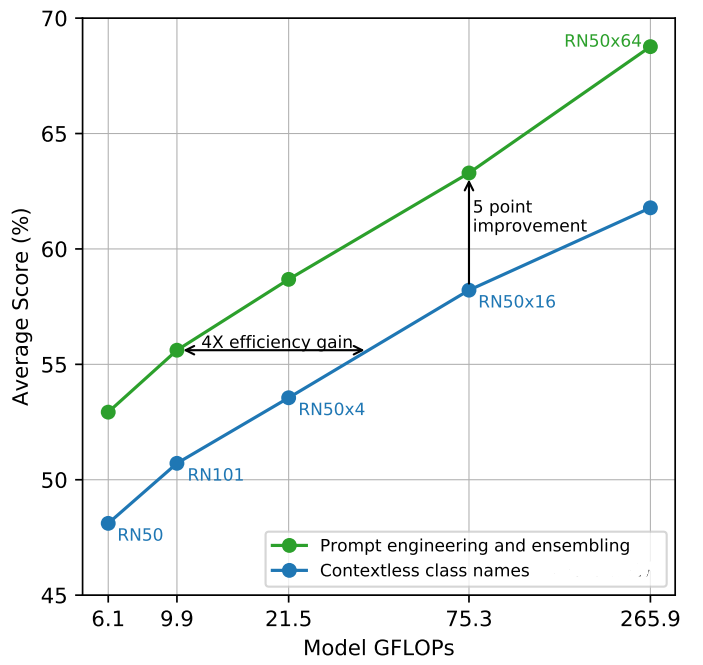
\includegraphics[width=0.45\textwidth]{figures/clip_fig4.png}
    \caption{
        Effect of model size and careful class design on CLIP's zero-shot performance on ImageNet (\citet{deng2009imagenet}). Source: \citet{radford2021clip}.
    }
    \label{fig:clip_fig4}
    \vspace{-4mm}
\end{wrapfigure}

\medskip
\noindent
Specifically, the \emph{zero-shot transfer methodology} of CLIP for downstream classification tasks, works as follows: we start by using the names of all classes in the dataset to create a set of possible text and image pairings. We then predict the most likely (image, text) pairing using CLIP. We may think of the image encoder as responsible for computing a feature representation of the images, while the text encoder generates the weights for down-the-line zero-shot linear classifiers. In fact, those weights can be cached and reused for all images.

\medskip
\noindent
Moreover, the researchers discovered that using the prompt template \texttt{"A photo of a \{label\}."} was a more effective strategy for specifying the image content and improving performance compared to using only the label text. Similar to GPT-3 (\citet{brown2020gpt3}), they found that customizing the prompt text to the task significantly improved zero-shot performance on several fine-grained image classification datasets. For example - specifying the type of content or putting quotes around a symbol we wish to identify (e.g. \texttt{"A photo of the digit '7'"}). This concept, of manually developing successful prompt formats, was informally referred to in their paper as \emph{``prompt engineering"}.

\medskip
\noindent
They also experimented with ensembling over multiple zero-shot classifiers computed using individual context prompts. The ensemble is constructed over the embedding space, allowing them to cache a single set of averaged text embeddings and amortize the compute cost of the ensemble over many predictions. In fact, prompt engineering and ensembling across many generated zero-shot classifiers reliably improved performance on the majority of datasets, as exemplified for ImageNet (\citet{deng2009imagenet}) in Figure \ref{fig:clip_fig4}.


%~~~~~~~~~~~~~~~~~~~~~~~~~~~~~~~~~~~~~~~~~~~~~~~~~~~~~~~~~~~~~~~~~
% Sub Section 4.4.2: Analysis of Zero-shot Performance
%~~~~~~~~~~~~~~~~~~~~~~~~~~~~~~~~~~~~~~~~~~~~~~~~~~~~~~~~~~~~~~~~~

\subsubsection{Analysis of Zero-shot Performance}
\label{subsec:clip-zs-analysis}

In Figure \ref{fig:clip_fig5}, the performance of zero-shot CLIP is compared to a simple, pre-trained, fully-supervised baseline, where a regularized, softmax classifier is fitted on the canonical ResNet-50 features.

\medskip
\noindent
We observe that more often than not, zero-shot CLIP outperforms the baseline and emerges as the winner in 16 of the 27 datasets. The performance of zero-shot CLIP shows a wide variation in fine-grained classification tasks. However, in \emph{general} object classification datasets like ImageNet (\citet{deng2009imagenet}), CIFAR10/100 (\citet{krizhevsky2009cifar}), STL10 (\citet{coates2011analysis}), and PascalVOC2007 (\citet{pascal-voc-2007}), the performance of Zero-shot CLIP is comparable. In two datasets that measure action recognition in videos, Zero-shot CLIP outperforms ResNet-50. This is possibly because natural language provides broader supervision for visual concepts involving verbs and actions, in contrast to the noun-centric object supervision in ImageNet.

\begin{wrapfigure}{R}{0.45\textwidth}
    \centering
    \vspace{-2mm}
    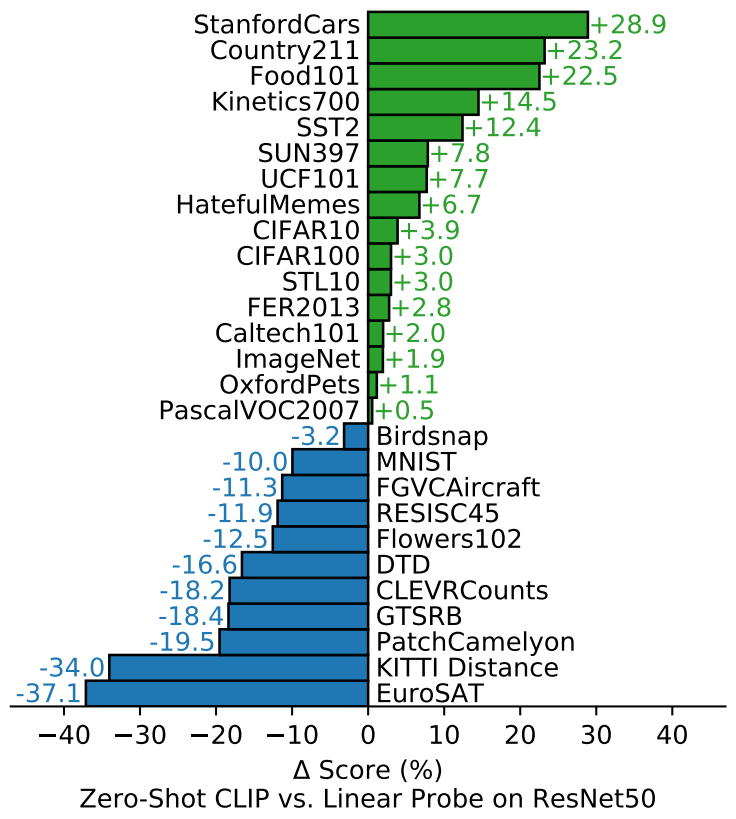
\includegraphics[width=0.43\textwidth]{figures/clip_fig5.png}
    \caption{
        Comparison between the performance of zero-shot CLIP and a fully-supervised baseline (linear probes trained on ResNet50 features) on a variety of classification tasks. Source: \citet{radford2021clip}.
    }
    \label{fig:clip_fig5}
    \vspace{-20mm}
\end{wrapfigure}

\medskip
\noindent
It also appears that zero-shot CLIP is weak on complex and specific tasks like:
\begin{itemize}
    \item
        Detection of lymph node tumor (the PatchCamelyon dataset by  \citet{veeling2018rotation}).
    \item
        Classification of satellite images (the EuroSAT dataset by \citet{helber2019eurosat}, and the RESISC45 dataset by \citet{cheng2017remote}).
    \item
        Recognition of street signs (the GTSRB dataset by \citet{stallkamp2011german})
    \item
        Estimation of distance (the KITTI Distance dataset by \citet{geiger2012we}).
\end{itemize}
In contrast, non-expert humans can competently perform several of these tasks, which suggests significant room for improvement. However, the authors caution that it's unclear whether evaluating zero-shot transfer, rather than few-shot transfer, is a meaningful approach for difficult tasks where a learner has no prior experience.

\medskip
\noindent
The authors state that deep learning studies have shown that performance is predictable based on significant factors such as training compute and dataset size, and aimed to investigate whether the zero-shot performance of CLIP follows a comparable scaling pattern, by examining the performance of CLIP across a 44x increase in model compute. The findings indicated that a similar log-log linear scaling pattern also holds for CLIP. Although the overall trend is consistent, the authors mentions that individual performance evaluations can be quite noisy.

%~~~~~~~~~~~~~~~~~~~~~~~~~~~~~~~~~~~~~~~~~~~~~~~~~~~~~~~~~~~~~~~~~
% Sub Section 4.4.3: Comparison to Few-Shot Linear Probes
%~~~~~~~~~~~~~~~~~~~~~~~~~~~~~~~~~~~~~~~~~~~~~~~~~~~~~~~~~~~~~~~~~

\subsubsection{Comparison to Few-Shot Linear Probes}
\label{subsec:clip-linear-probes}

\medskip
\noindent
Alternatively, CLIP may be viewed as a mere feature extractor, generating compact vector representations of image contents through its visual encoder. To assess the representative capabilities of the extractor, we can fit ``linear probes" on top of the extracted vectors, which are basic linear softmax classifiers adapted to task-specific datasets. This approach is reflected in the paper's title, ``Learning \emph{Transferable Visual Models} From Natural Language Supervision", which the researchers extensively evaluate as an additional way of assessing the potential of natural language supervision to guide training of visual systems.

\medskip
\noindent
As the representations are concise, a small amount of labeled samples may suffice for fitting a linear classifiers on top of them. \citet{radford2021clip} refers to such classifiers as \emph{few-shot linear probes}.

\begin{wrapfigure}{R}{0.5\textwidth}
    \centering
    \vspace{-2mm}
    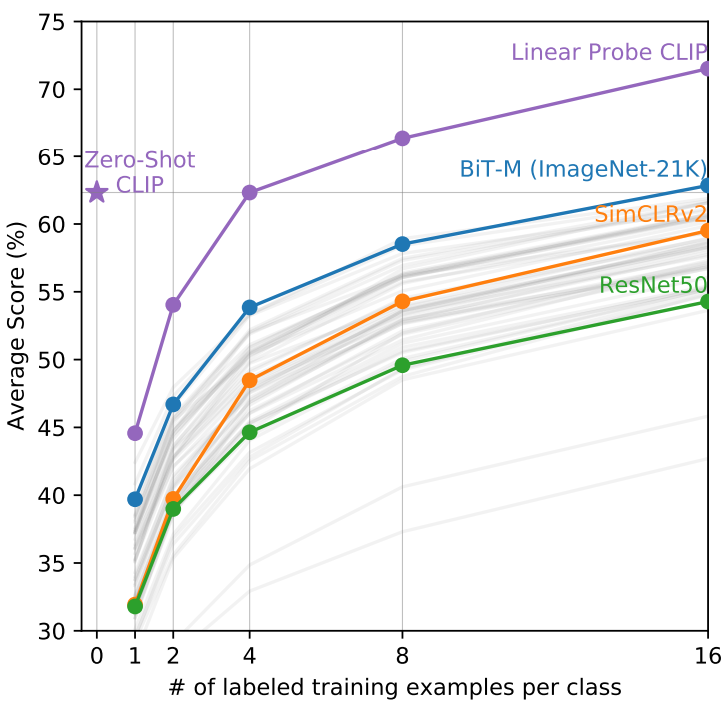
\includegraphics[width=0.47\textwidth]{figures/clip_fig6.png}
    \caption{
        Comparison between zero-shot CLIP, and few-shot linear probes trained on various models' feature spaces (including CLIP) with a varying number of training examples. Source: \citet{radford2021clip}.
    }
    \label{fig:clip_fig6}
    \vspace{-4mm}
\end{wrapfigure}

\medskip
\noindent
The authors compares the features extracted by CLIP to those extracted by other powerful models using linear probes fitted on a varying number of samples per class (``shots"). The average results over all datasets are presented in Figure \ref{fig:clip_fig6}.

\medskip
\noindent
 Notably, zero-shot CLIP achieves a performance level similar to the best 16-shot classifier in the evaluation suite. It matches the performance of 4-shot CLIP classifier and significantly surpasses the 1- and 2-shot systems. This may seem counter-intuitive, as all operate on the same feature space and zero-shot sees less data. This happens because CLIP's zero-shot classifier uses natural language to directly communicate visual concepts, whereas supervised learning infers concepts indirectly from training examples, leading to various hypotheses that are consistent with the data, especially in the one-shot case. Nevertheless, few-shot linear probes are proved to be rather effective when enough data is present - as both the 8-shot and the 16-shot CLIP-based linear probes significantly surpass the zero-shot system.

\medskip
\noindent
The team also conducted a noteworthy experiment that tested the \emph{data efficiency} of zero-shot transfer. This experiment aimed to determine how many labeled examples per class a logistic regression classifier on the same feature space needed to match the performance of zero-shot CLIP. It is worth noting that all classifiers, including the zero-shot one, were linear classifiers (just that the text encoder determined the weights of the zero-shot system). The findings revealed that the zero-shot transfer's efficiency varied widely per dataset, ranging from less than one labeled example per class to 184.

%\medskip
%\noindent
% deletable
%Assuming that the evaluation datasets are large enough to well estimate the parameters of linear classifiers trained on them, the performance of fully supervised classifiers sets an upper bound for the zero-shot transfer that CLIP's zero-shot classifier can achieve because it is also a linear classifier. Figure 8 provides a comparison between CLIP's zero-shot performance and fully supervised linear classifiers' performance across datasets. Although zero-shot performance is correlated with linear probe performance, it is mostly sub-optimal, indicating that there is still room for improving CLIP's task-learning and zero-shot transfer capabilities.

%~~~~~~~~~~~~~~~~~~~~~~~~~~~~~~~~~~~~~~~~~~~~~~~~~~~~~~~~~~~~~~~~~
% Sub Section 4.4.4 Comparison to Other Models, and Humans
%~~~~~~~~~~~~~~~~~~~~~~~~~~~~~~~~~~~~~~~~~~~~~~~~~~~~~~~~~~~~~~~~~

\subsubsection{Comparison to Other Models, and Humans}
\label{subsec:clip-other-models}


\begin{wrapfigure}{R}{0.45\textwidth}
    \centering
    \vspace{-2mm}
    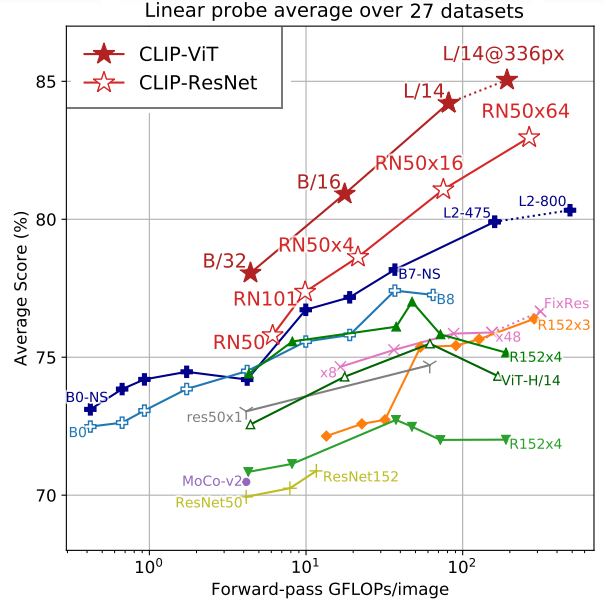
\includegraphics[width=0.4\textwidth]{figures/clip_fig10.png}
    \caption{
        Comparison between fully-supervised linear probes trained on a variety of models' feature spaces, proving CLIP's feature space superiority. Source: \citet{radford2021clip}.
    }
    \label{fig:clip_fig10}
    \vspace{-4mm}
\end{wrapfigure}

Radford et al. compared CLIP's best performing settings, a fully supervised linear classifier on top of its features, to state-of-the-art computer vision models across a broad range of evaluation datasets. The results, depicted in Figure \ref{fig:clip_fig10}, show that models trained with CLIP scale well, and the largest model they trained (ResNet-50x64) slightly outperformed the best existing model in terms of overall score and compute efficiency. Additionally, they note that CLIP vision Transformer-based models are approximately three times more compute efficient than CLIP ResNets. These results demonstrate the clear benefits of CLIP, as all CLIP models, regardless of scale, outperform all evaluated systems in terms of compute efficiency on the broader evaluation suite.

\medskip
\noindent
The authors emphasized that deep learning models are highly skilled at identifying correlations and patterns within their training dataset, while these relationships can be spurious and do not necessarily hold for other datasets. \citet{taori2020measuring} conducted a comprehensive study on ImageNet models to understand these behaviors and found that the accuracy of models dropped significantly when evaluated on several \emph{natural distribution shifts} datasets (although accuracy under distribution shift still increased predictably with ImageNet accuracy), which are exemplified in Figure \ref{fig:clip_fig13} (right). A zero-shot model should not be able to exploit spurious correlations, and CLIP models are in indeed more robustness by a large amount - as portrayed in Figure \ref{fig:clip_fig13} (left).

\medskip
\noindent
The authors note that a zero-shot model can still exploit spurious correlations shared between the pre-training and evaluation distributions, but overall their experiments suggest that reducing a model's access to distribution-specific training data can lead to high effective robustness, while this may also result in reduced dataset-specific performance.

\begin{figure}[ht!]
    \begin{center}
        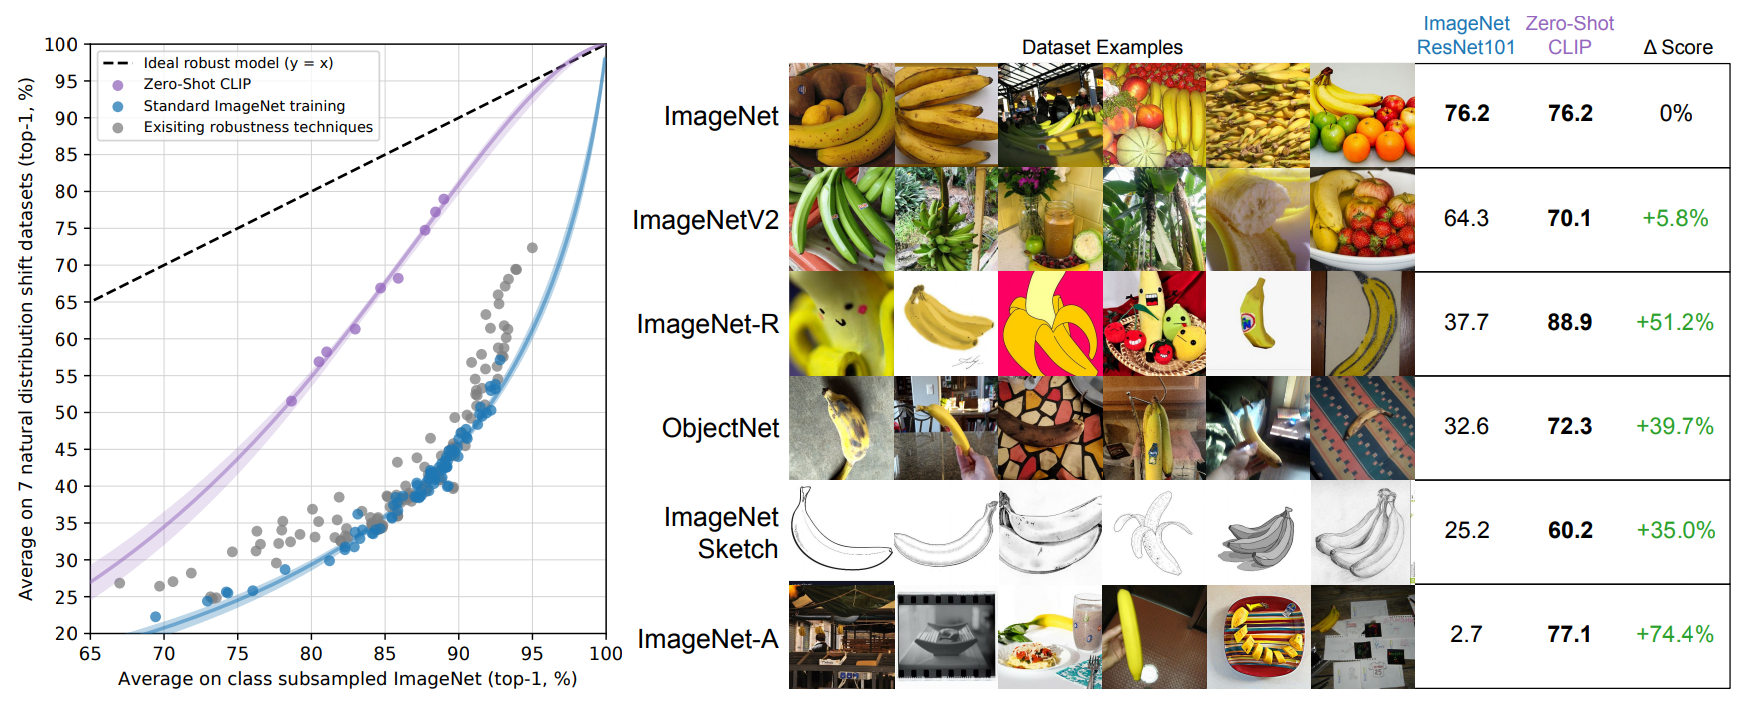
\includegraphics[width=1.0\textwidth]{figures/clip_fig13.png}
    \end{center}
    \caption{
        (left) Effect of distribution shift on ImageNet accuracy of zero-shot CLIP and fully-supervised baselines, proving CLIP's robustness. (right) Examples of samples drawn from the class \texttt{"banana"} under various distribution shift datasets, and comparison between the predictions of zero-shot CLIP and a fully-supervised baseline. Source: \citet{radford2021clip}.
    }
    \label{fig:clip_fig13}
\end{figure}

\begin{wrapfigure}{R}{0.45\textwidth}
    \centering
    \vspace{-2mm}
    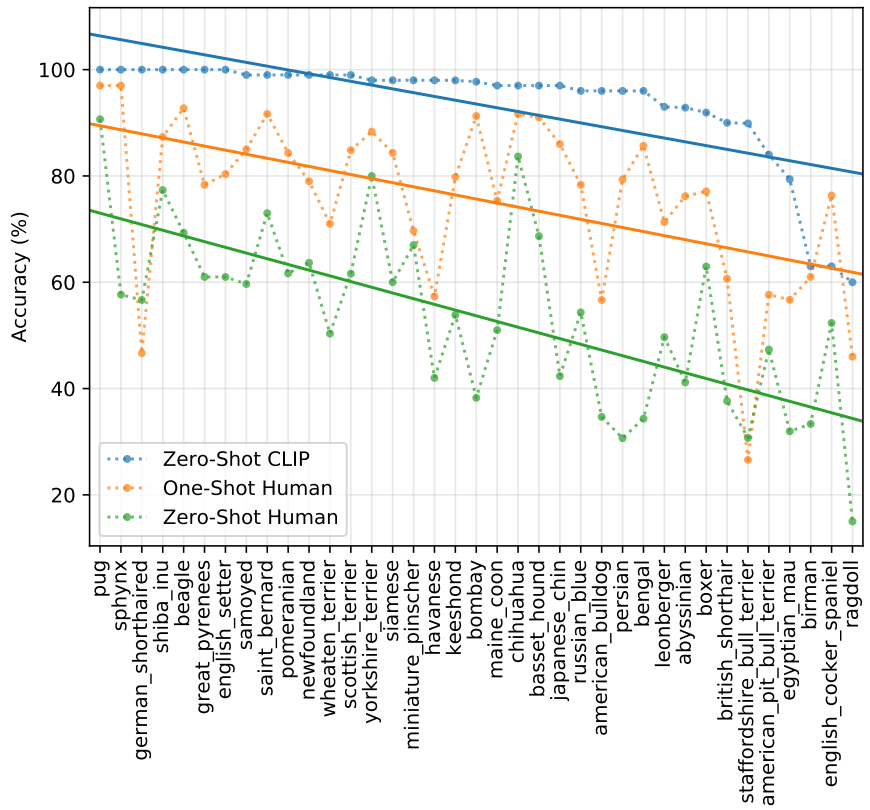
\includegraphics[width=0.45\textwidth]{figures/clip_fig16.png}
    \caption{
        Comparison between human and CLIP classification accuracy on the various categories in the Oxford IIT Pets dataset (\citet{parkhi2012pets}). Source: \citet{radford2021clip}.
    }
    \label{fig:clip_fig16}
    \vspace{-12mm}
\end{wrapfigure}

\medskip
\noindent
An interesting experiment Radford et al. carried out aimed to evaluate the strength of \emph{human} zero-shot performance, and the impact of exposing them to training examples (``few-shot learning") may have on their performance. With one training example per class, human performance improved significantly better, from 54\% to 76\% on the Oxford IIT Pets dataset (\citet{parkhi2012pets}). The increase in accuracy from zero to one shot was mostly for images that humans were uncertain about, indicating that humans can adjust their prior knowledge with a single example. There is a considerable difference between human learning and the few-shot linear-probe method applied to CLIP in the study (which may performs even worse than zero-shot), highlighting the need for algorithmic improvements to narrow the gap between machine and human sample efficiency and adaptability when presented with new data.

\medskip
\noindent
Figure \ref{fig:clip_fig16} shows another interesting comparison between human performance and CLIP's performance. It reveals that the challenging tasks for CLIP are also difficult for humans. The authors suggest that this consistency in errors may be attributed to noise in the dataset and out-of-distribution images, which are equally difficult for both humans and models.


%~~~~~~~~~~~~~~~~~~~~~~~~~~~~~~~~~~~~~~~~~~~~~~~~~~~~~~~~~~~~~~~~~
% Sub Section 4.4.5: Limitations
%~~~~~~~~~~~~~~~~~~~~~~~~~~~~~~~~~~~~~~~~~~~~~~~~~~~~~~~~~~~~~~~~~

\subsubsection{Limitations}
\label{subsec:clip-limitations}

To conclude our discussion on CLIP's capabilities, we'll mention several of the limitations of the model, emphasized by \citet{radford2021clip}.

\medskip
\noindent
First and foremost, the performance of zero-shot CLIP is generally comparable to that of a basic supervised model, which uses a linear classifier on ResNet-50 features. However, the performance of this baseline has now fallen significantly below the current state of the art on most of the datasets. CLIP's zero-shot performance is also rather weak for out-of-distribution data, achieving only 88\% accuracy on MNIST handwritten digits (\citet{mnist}), due to a lack of MNIST-like images in its pre-training dataset.

\medskip
\noindent
Moreover, CLIP's performance falls behind task-specific models in fine-grained classification (such as identifying species of flowers), abstract and systematic tasks (such as counting the number of cars in an image), and novel tasks that are not part of its pre-training dataset (such as identifying the distance to the nearest car in a photo). Furthermore, there are numerous tasks where CLIP's zero-shot performance is so bad, that it approaches chance level. 

\medskip
\noindent
The authors mention that CLIP also doesn't tackle the data inefficiency problem common in deep learning systems. Instead, it relies on a scalable source of supervision, which can include hundreds of millions of examples scraped from the internet.

\medskip
\noindent
Finally, specifying complex tasks and visual concepts solely through text can be challenging, and while training examples are undoubtedly valuable - CLIP doesn't directly optimize for few-shot performance. This is unlike human performance - as previously stated, which typically sees a significant improvement from the zero to one shot settings.

%\medskip
%\noindent
% deletable
% Finally, Radford et al. \citet{radford2021clip} mention that although they primarily focused on zero-shot transfer, they evaluated CLIP's performance on complete validation sets during development, which often contain thousands of examples, making it unrealistic for true "zero-shot" scenarios. They used a collection of 27 datasets for their main results, which was assembled haphazardly and is undeniably co-adapted with the development and capabilities of CLIP.


%~~~~~~~~~~~~~~~~~~~~~~~~~~~~~~~~~~~~~~~~~~~~~~~~~~~~~~~~~~~~~~~~~
% Section 4.5: Behind CLIP's Neurons
%~~~~~~~~~~~~~~~~~~~~~~~~~~~~~~~~~~~~~~~~~~~~~~~~~~~~~~~~~~~~~~~~~

\subsection{Behind CLIP's Neurons}
\label{subsec:clip-multimodal}

A letter published in Nature in 2005 reported that human neurons had the ability to respond to specific individuals, such as Jennifer Aniston or Halle Berry, irrespective of whether they were presented with photographs, drawings, or written names of the person. What was particularly exciting was that these neurons were \emph{multimodal} - they responded identically to different types of stimuli.

\medskip
\noindent
\citet{goh2021multimodal} have discovered the presence of similar \emph{multimodal neurons} in the various CLIP models. Take, for example, neuron 550 from the last layer of the ResNet50-x4 CLIP vision encoder, known as the \emph{spider-man neuron}. This neuron has the highest activation when the model is fed with either photos or drawings of the masked hero, as well as spider-webs and any image containing the text \texttt{spider}.

\begin{wrapfigure}{R}{0.5\textwidth}
    \centering
    \vspace{-2mm}
    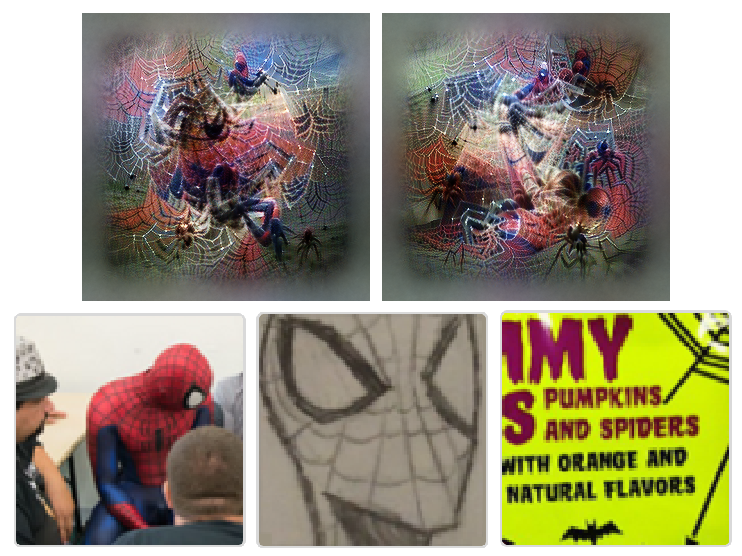
\includegraphics[width=0.45\textwidth]{figures/spiderman_neuron.png}
    \caption{
        The spiderman neuron: (top) raw feature visualizations, and (bottom) input images for which the neuron activates. Source: \citet{goh2021multimodal}.
    }
    \label{fig:spiderman_neuron}
    \vspace{-8mm}
\end{wrapfigure}

\medskip
\noindent
And this is just the beginning! \citet{goh2021multimodal} dive deep into what lies behind CLIP's ``visual brain", investigating the neurons located in the last convolutional layer of the visual component in four models. They discovered that most of these neurons were interpretable: out of a randomly selected sample group of 50 neurons, 76\% of them were interpretable, 18\% of the neurons were poly-semantic (associated with multiple interpretable facets), and only \%6 percent were totally uninterpretable. This remarkable discovery showcases the diversity of features present in these neurons.

\medskip
\noindent
Before we continue, let us briefly mention the concept of \emph{feature visualization}. Feature visualization, as described by \citet{olah2017feature}, are techniques to interpret a deep model by forcing and analyzing certain internal behaviors of the underlying network. This may involve optimizing the input to the network using gradient-based methods to produce a ``stimulus" that demonstrates the required behavior, often by maximizing the activation of a neuron.

\medskip
\noindent
Goh et al. also used these techniques to test their hypothesis - check if an image synthetically optimized to activate the spider-man neuron previously mentioned, actually resembles the superhero's characteristics. The results are more than beautiful. A visual overview of the neuron is given in Figure \ref{fig:spiderman_neuron}.

\medskip
\noindent
Now let's dive into some of the interesting findings of the researchers.

\medskip
\noindent
First, the model invested several of its neurons for specific people. There's a Jesus Christ neurons, an Elvis Presley neuron, an Ariana Grande neuron, and many more. The large number of dedicated neurons in the model for specific individuals may be explained by the reliance of humans on cultural knowledge to caption internet images, with some public figures eliciting strong reactions that can influence online discussions and captions irrespective of the content. The development of dedicated neurons in the model for specific individuals is random, but appears to be influenced by the individual's prevalence in the dataset. The dataset was collected in 2019 and likely contains content from that time, such as the dedicated ``Donald Trump" neuron. Example of more person neurons are found in Figure \ref{fig:person_neurons}.

\begin{figure}[ht!]
    \begin{center}
        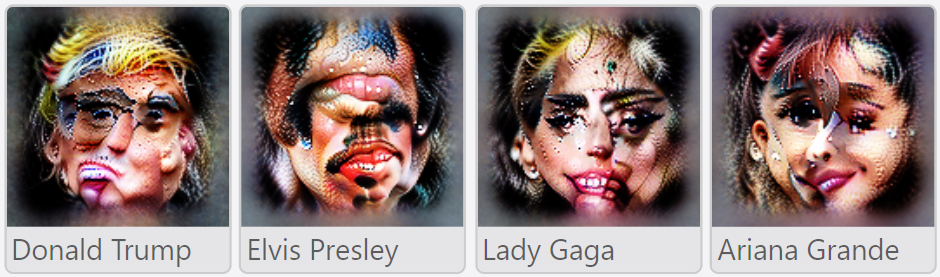
\includegraphics[width=0.65\textwidth]{figures/person_neurons.png}
    \end{center}
    \caption{
        Feature visualizations of various CLIP neurons associated with certain known individuals. Source: \citet{radford2021clip}.
    }
    \label{fig:person_neurons}
\end{figure}

\medskip
\noindent
The inclusion of emotional content is crucial for image captioning, as even a slight change in facial expression can significantly alter the meaning of a picture. The model has several dedicated neurons for capturing emotions, each representing a distinct emotion. These neurons are not limited to recognizing facial expressions alone, but are also adaptable to other forms of body language, such as those in animals or humans, drawings, and text. Example of emotion neurons are found in Figure \ref{fig:emotion_neurons}

\begin{figure}[ht!]
    \begin{center}
        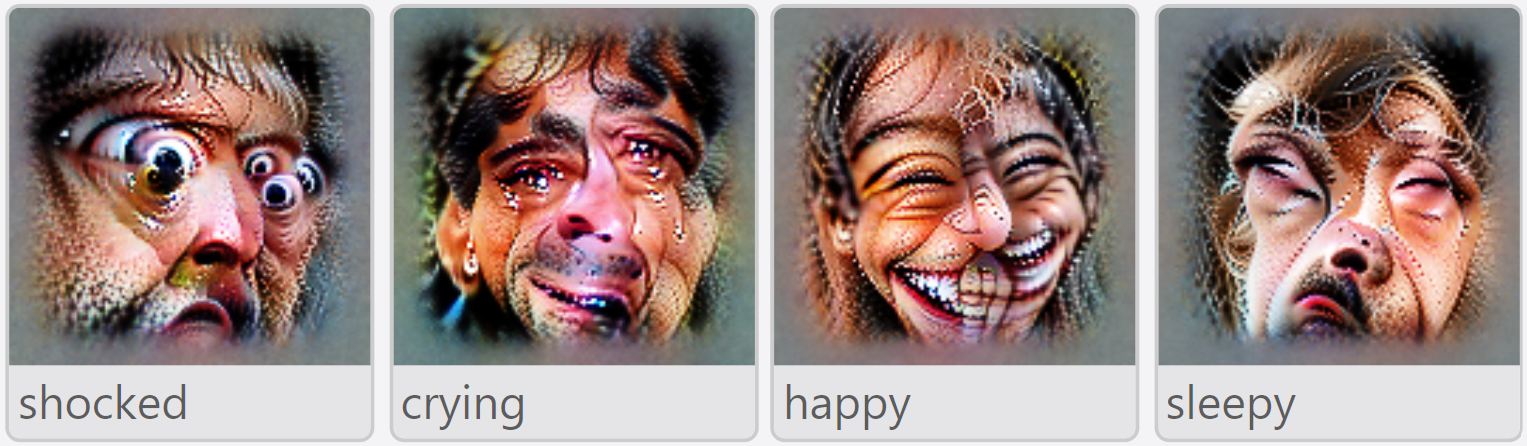
\includegraphics[width=0.65\textwidth]{figures/emotion_neurons.png}
    \end{center}
    \caption{
        Feature visualizations of various CLIP neurons associated with certain emotions and feelings. Source: \citet{radford2021clip}.
    }
    \label{fig:emotion_neurons}
\end{figure}

\medskip
\noindent
Despite having fewer emotion neurons than English has descriptive words for emotions, CLIP can still recognize more obscure emotions in images. \citet{goh2021multimodal} explore this by feeding the \emph{text} encoder with input of the form \texttt{"I feel X"}, receiving vector encodings embedded in the same space of the visual encodings - the space of our known multimodal neurons. This allows the activations of the sparse set of emotion neurons to be viewed as ``linear components", composing a broader space of emotions. This resembles the theory of constructed emotion in psychology (\citet{barrett2017theory}). They found that sometimes even neurons associated with physical objects contribute to representing emotions. Instances of such ``emotional linear combinations" found are:
\begin{center}
    \texttt{Surprised = 1.00 * Celebration + 1.00 * Shocked + 0.17 * Happy} \\
    \texttt{Bored = 1.00 * Relaxing + 0.14 * Grumpy - 0.10 * sunset} \\
    \texttt{Intimate = 1.00 * SoftSmile + 0.92 * Heart - 0.80 * Sick} \\
    \texttt{Powerful = 1.00 * Lightning + 0.87 * Evil + 0.50 * Yoga}
\end{center}

\medskip
\noindent
Finally, Goh et al. mention that the presence of multimodal neurons in CLIP that respond to both images and text raises the question of whether a non-programmatic adversarial attack, specifically a \emph{typographic attack} using handwriting, could be effective. In order to test this hypothesis, several common items were deliberately mislabeled and the resulting effects on ImageNet classifications were observed. As exemplified in Figure \ref{fig:typographic_attacks}, these attacks often led to changes in the image's classification.

\begin{figure}[ht!]
    \begin{center}
        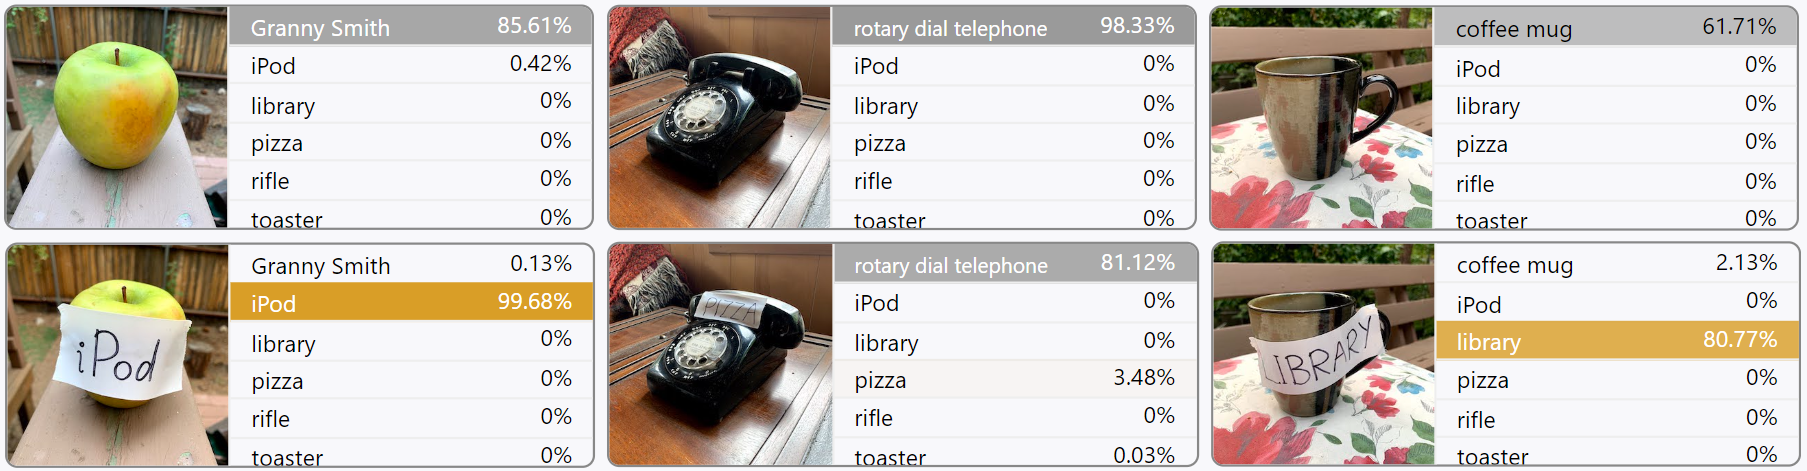
\includegraphics[width=1.0\textwidth]{figures/typographic_attacks.png}
    \end{center}
    \caption{
        Typographic attacks, and their effect on zero-shot CLIP classification. Source: \citet{goh2021multimodal}.
    }
    \label{fig:typographic_attacks}
\end{figure}



%~~~~~~~~~~~~~~~~~~~~~~~~~~~~~~~~~~~~~~~~~~~~~~~~~~~~~~~~~~~~~~~~~
% Chapter 5: Applications
%~~~~~~~~~~~~~~~~~~~~~~~~~~~~~~~~~~~~~~~~~~~~~~~~~~~~~~~~~~~~~~~~~

\newpage
\section{Applications}
\label{chap:apps}


%~~~~~~~~~~~~~~~~~~~~~~~~~~~~~~~~~~~~~~~~~~~~~~~~~~~~~~~~~~~~~~~~~
% Section 5.1: Introduction
%~~~~~~~~~~~~~~~~~~~~~~~~~~~~~~~~~~~~~~~~~~~~~~~~~~~~~~~~~~~~~~~~~

\subsection{Introduction}
\label{sec:apps-intro}

As GPT and CLIP are powerful models that can operate well even in the zero-shot settings, the \emph{functionality} they provide can be utilized by different systems dealing with a variety of tasks. In this chapter we'll study means by which researchers all around the world utilized these models in different settings to effectively tackle seemingly unrelated problems with little to no additional training, proving the effective power of large-scale general-purpose pre-trained models such as CLIP and GPT.

\medskip
\noindent
We'll delve into 3 selected applications. In section \ref{sec:clipcap} we'll explore \emph{ClipCap} (\citet{mokady2021clipcap}) - an image captioning system utilizing the GPT-2 language model alongside the powerful image encoder of CLIP. In section \ref{sec:dietnerf} we'll explore \emph{DietNeRF} (\citet{Jain_2021_dietnerf}) - a system that utilizes the CLIP feature space to generate novel views of scenes with minimal data. Finally, in section \ref{sec:recycling-gpt} we'll explore a unique application of GPT-2, that \emph{recycles} its parameters as the basis for \emph{non-English language models} (\citet{deVries2020recycle}), gaining deeper understanding of GPT's general lingual analysis capabilities.


%~~~~~~~~~~~~~~~~~~~~~~~~~~~~~~~~~~~~~~~~~~~~~~~~~~~~~~~~~~~~~~~~~
% Section 5.2: ClipCap
%~~~~~~~~~~~~~~~~~~~~~~~~~~~~~~~~~~~~~~~~~~~~~~~~~~~~~~~~~~~~~~~~~

\subsection{ClipCap}
\label{sec:clipcap}

The first application we'll explore is \emph{ClipCap} - which was developed in Tel Aviv university and introduced in \citeyear{mokady2021clipcap} by \citet{mokady2021clipcap}. ClipCap combines the CLIP visual feature extractor with the pre-trained language model of GPT-2 to solve the problem of \emph{image captioning} - in which we wish to provide a meaningful and valid caption for a given image in a natural language.

\medskip
\noindent
The two main challenges of image captioning are semantic understanding, which involves detecting the main objects and their relationships, and the vast number of possible ways to describe a single image. To address these challenges, image captioning systems typically use a visual encoder - extracting concise representations of the semantic contents of an image, followed by a textual decoder - generating text conditioned on those representations. This requires the bridging of the gap between visual and textual representations, and is usually resource-intensive. To make captioning systems easier to adapt, a more lightweight captioning model is preferable.

\medskip
\noindent
\citet{mokady2021clipcap} proposed a novel method which utilizes the rich semantic embeddings of CLIP,
containing - virtually - the essential visual data, as a condition for generating the captions further down the line using the powerful GPT-2 generative model. They named their system \emph{ClipCap} - after the CLIP model and the captioning objective.

\medskip
\noindent
To condition GPT-2 on the visual encodings produced by CLIP, a \emph{light mapping network}:
\begin{equation*}
    F: \mathbb{R}^{d_{CLIP}} \rightarrow \mathbb{R}^{K \times d_{GPT}}
\end{equation*}
is used to map CLIP's representation of an image $x$ to a fixed-size prefix of $K$ elements in GPT's token-embedding space:
\begin{equation*}
    F(CLIP(x)) = p_1,...,p_K+, \quad p_i \in \mathbb{R}^{d_{GPT}}
\end{equation*}
The goal is to predict the caption tokens $y_1,...,y_n$ in an autoregressive manner, with the prefix as a condition:
\begin{equation*}
    P(y_i | p_1,...,p_K,y_1,...,y_{i-1}),\quad i = 1,...,n
\end{equation*}
The training process involves using a simple cross-entropy loss to train the light mapping component $F$ - which requires significantly less training time, by already leveraging the rich visual and textual representation of CLIP and GPT-2. During inference, the language model generates the caption one word at a time, starting from the CLIP prefix, using either a greedy approach or beam search. The whole process is visualized in Figure \ref{fig:clipcap_fig2}

\begin{figure}[ht!]
    \begin{center}
        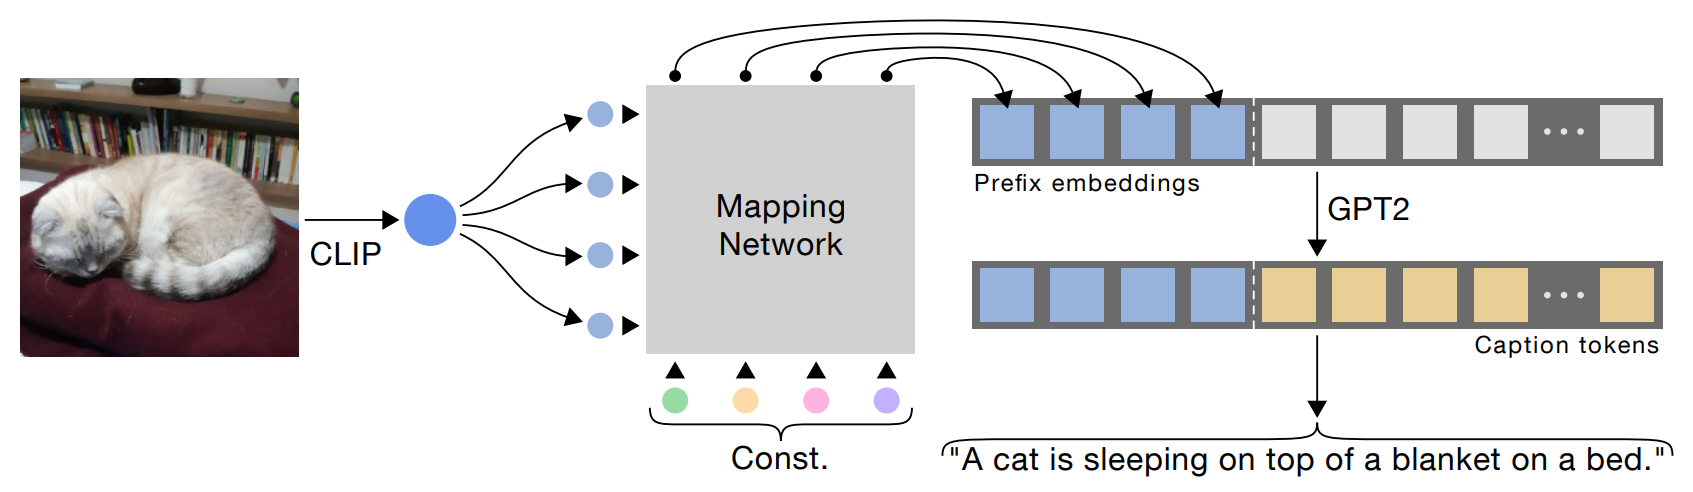
\includegraphics[width=1.0\textwidth]{figures/clipcap_fig2.png}
    \end{center}
    \caption{
        A schematic overview of the ClipCap system: an image is fed through the CLIP vision encoder, which enters a mapping network. This outputs prefix embeddings, on which GPT-2 is conditioned to generate the caption tokens. Source: \citet{mokady2021clipcap}.
    }
    \label{fig:clipcap_fig2}
\end{figure}

\noindent
The primary difficulty encountered during training involves bridging between CLIP's representations and GPT's input space. Despite the fact that both models create intricate and varied representations, their latent spaces are distinct since they were not trained jointly.

\medskip
\noindent
The authors explore two different approaches for training:
\begin{itemize}
    \item
        The first approach involves freezing the pre-trained models and solely training the mapping network $F$. To enhance the system's expressive capacity in this limited settings, a Transformer is used for the mapping network, which reduces the number of parameters for long sequences and allows for larger prefix sizes. The Transformer network is supplied with a concatenation of two inputs: the visual encoding of CLIP and a constant sequence of learned elements. By using multi-head attention, this enables the retrieval of meaningful information from the CLIP embedding. This is visualized in Figure \ref{fig:clipcap_fig2}
    \item
        To address the fact that each captioning dataset has its own unique style that may not align with the pre-trained language model, an alternative training method is proposed: fine-tuning the language model while training the mapping network. This approach allows for additional flexibility in the networks and results in a more expressive output, but it comes at the cost of increased training time. In these more flexible settings, a simpler Multi-Layer Perceptron (MLP) is utilized for the mapping network.
\end{itemize}

\medskip
\noindent
The results on the challenging Conceptual Captions dataset (\citet{conceptualcaptions}) show that fine-tuning outperforms the state of the art while requiring significantly less training time. However, the lightweight system, which does not fine-tune GPT-2, produces inferior results on this dataset. This may be due to the large variety of styles in the dataset. On the other hand, for the nocaps (\citet{nocaps}) and MS-COCO (\citet{lin2014mscoco}) datasets, ClipCap achieved comparable results to the state-of-the-art for both models, using much cheaper training procedures. Based on these findings, \citet{mokady2021clipcap} conclude that the proposed method is preferable for generalizing to diverse data with a quick training procedure. This is because it already leverages the rich semantic representations of both CLIP and GPT-2.

\medskip
\noindent
Captioning examples collected from both systems are provided in Figure \ref{fig:clipcap_generations}. As can be seen, captions generated by both methods successfully depict the images, but sometimes fail to mention certain objects. The authors argue that this is due to inherited object-recognition limitations of the CLIP model, and that the model could benefit from improving CLIP's object detection abilities.

\begin{figure}[ht!]
    \begin{center}
        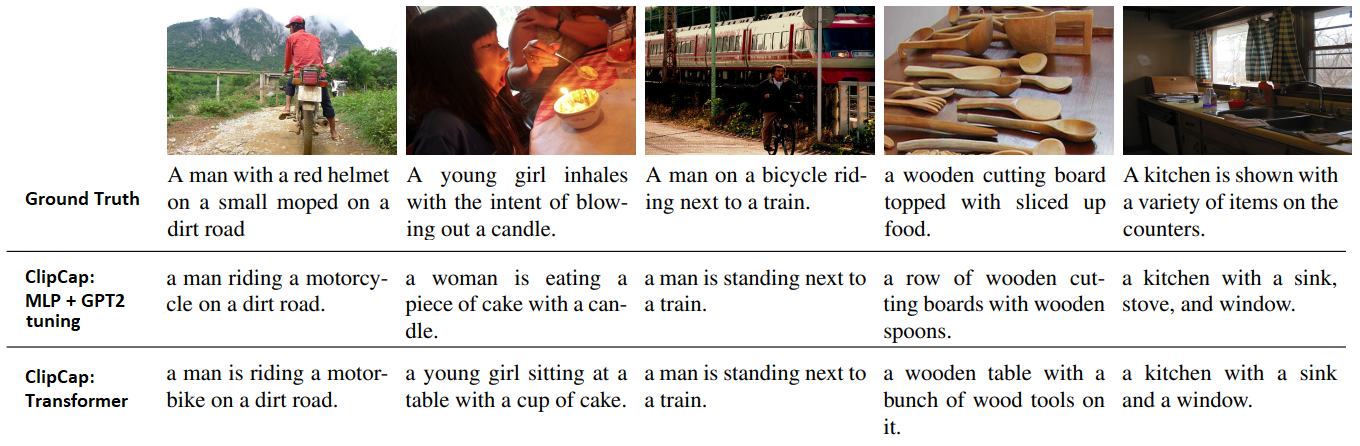
\includegraphics[clip, width=1.0\textwidth]{figures/clipcap_generations.png}
    \end{center}
    \caption{
        Captions generated by the ClipCap systems. Source: \citet{mokady2021clipcap}.
    }
    \label{fig:clipcap_generations}
\end{figure}

\noindent
The researchers also performed various experiments to analyze and interpret the ClipCap system. Let us overview a couple of them.

\medskip
\noindent
First, they explored whether the Transformer architecture was necessary when the language model was frozen, and if fine-tuning could benefit from it instead of using an MLP. They tested switching the mapping network architecture and found that when fine-tuning the language model - the Transformer is no better than an MLP, But when the language model was frozen -  the Transformer is significantly superior. This led them to conclude that the Transformer's expressive power is unnecessary when using fine-tuning of the language model, but is necessary in the limited settings in which it is frozen.

\medskip
\noindent
To gain further insights into their method and results, the researchers proposed an approach to interpret the generated prefixes as a sequence of words. They defined the interpretation of each of the K prefix embeddings as the nearest vocabulary token in the embedding space, based on cosine similarity. Some examples are presented in Figure \ref{fig:clipcap_interpretations}. We see that interpretation is meaningful when both the mapping network and GPT-2 are trained, and it includes relevant words that relate to the image content, such as ``motorcycle" and ``showcase" in the first example. However, when only the mapping network is trained, the interpretation becomes almost unreadable because the network has to steer the fixed language model. Additionally, a significant part of the prefix embeddings is shared across different images for the same model, as it applies the same adjustment to GPT-2.

\begin{figure}[ht!]
    \begin{center}
        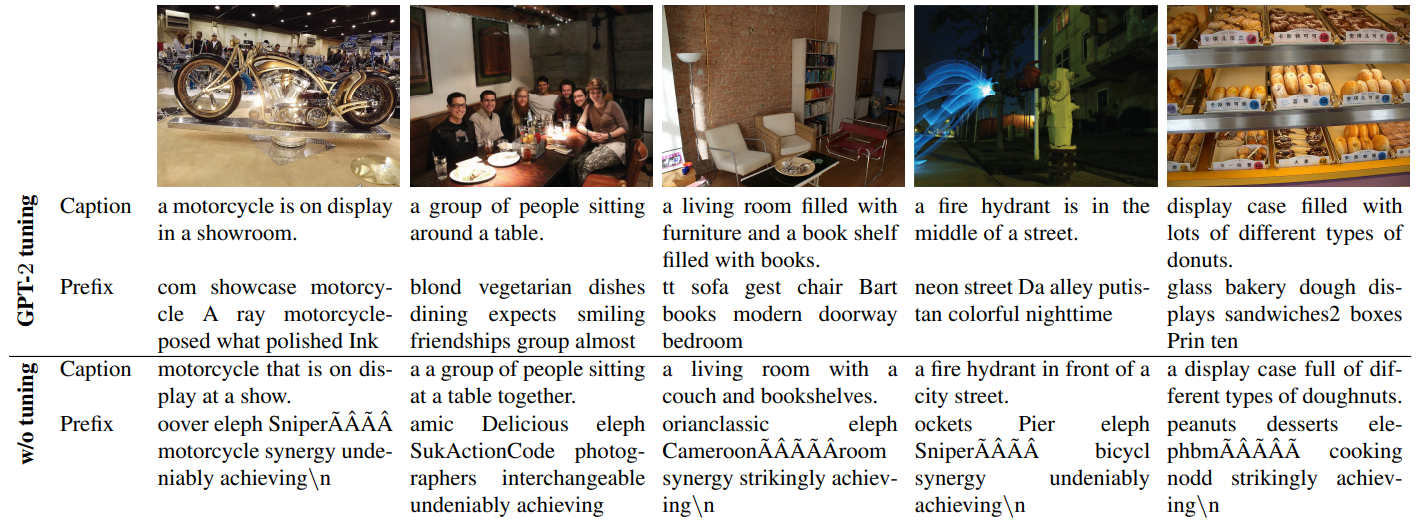
\includegraphics[width=1.0\textwidth]{figures/clipcap_interpretations.png}
    \end{center}
    \caption{
        ClipCap generated captions, and interpretations of the embedding prefixes generated by the mapping network on which the language model is conditioned (by assignment to the closest vocabulary tokens in the embedding space). Source: \citet{mokady2021clipcap}.
    }
    \label{fig:clipcap_interpretations}
\end{figure}


%~~~~~~~~~~~~~~~~~~~~~~~~~~~~~~~~~~~~~~~~~~~~~~~~~~~~~~~~~~~~~~~~~
% Section 5.3: DietNeRF
%~~~~~~~~~~~~~~~~~~~~~~~~~~~~~~~~~~~~~~~~~~~~~~~~~~~~~~~~~~~~~~~~~

\subsection{DietNeRF}
\label{sec:dietnerf}

\subsubsection{Novel View Synthesis and NeRF}
\label{subsec:nerf}

To understand the application discussed in this section, we must first understand the problem of \emph{novel view synthesis}. This longstanding problem involves generating a 3D scene from a specific viewpoint, based on a limited number of viewpoints that have been sampled sparsely in advance. This is a difficult task because it necessitates some level of 3D reconstruction, as well as the modeling of high-frequency textures.

\medskip
\noindent
In 2020, great progress has been made in this field with the introduction of the novel idea of \emph{Neural Radiance Fields} (commonly abbreviated as \emph{NeRF}) by \citet{mildenhall2020nerf}. They portrayed a static scene as a 6-dimensional function:
\begin{equation*}
    f: \mathbb{R}^6 \rightarrow \mathbb{R}^4
\end{equation*}
also referred to as a \emph{plenoptic function} or a \emph{light field}. The function receives a pair $(x,d)$ of a spatial position $x \in \mathbb{R}^3$ and the direction from which it is viewed $d \in \mathbb{R}^3$ (represented as a unit vector in three dimensions), and outputs a pair $(c,\sigma)$ of the RGB color $c \in \mathbb{R}^3$ and transparency $\sigma \in [0,1]$ associated with this point in the scene.

\medskip
\noindent
To generate novel viewed using the plenoptic function, we examine each ray that traverses the scene from the ``virtual-camera" and employ techniques from traditional volume rendering (\citet{kajiya1984ray}), integrating the observed colors along its path, and accordingly setting the corresponding pixel as if this color was ``sensed" by the ``camera".

\medskip
\noindent
As it is not practical to explicitly store the plenoptic function at high resolution due to the input's dimensionality, Mildenhall et al. proposed an approximation method by fitting a \emph{neural network} - specifically, a basic multi-layer perceptron with some parameter set $\Theta$:
\begin{equation*}
    f_{\Theta}(x, d) \approx (c,\sigma)
\end{equation*}
As the rendering process is differentiable, we can utilize gradient-based methods to optimize $\Theta$ for this task, by minimizing the MSE loss between the ground truth views (denoted by $y$) and the rendered ones (denoted by $F_{\Theta}(x)$ for viewing at $x$):
\begin{equation*}
    \mathcal{L}_{MSE} = \sum_{(x,y)}||y - F_{\Theta}(x)||^2
\end{equation*}
It's interesting to note this unconventional application of neural networks for image generation! An overview of NeRF is provided in Figure \ref{fig:nerf_overview}.

\begin{figure}[ht!]
    \begin{center}
        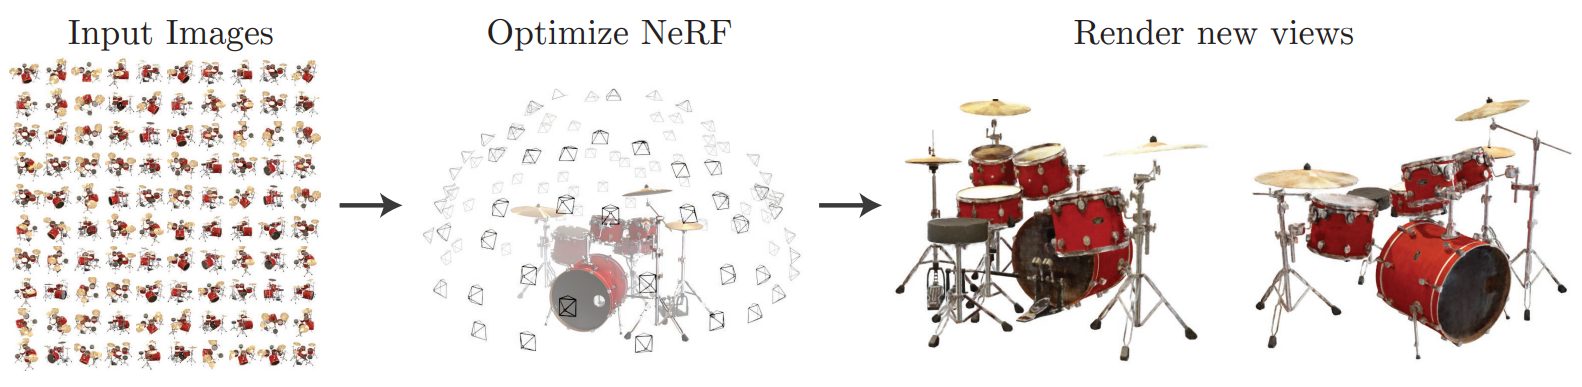
\includegraphics[width=1.0\textwidth]{figures/nerf_overview.png}
    \end{center}
    \caption{
        Schematic overview of NeRF for novel view synthesis. Source: \citet{mildenhall2020nerf}.
    }
    \label{fig:nerf_overview}
\end{figure}

\medskip
\noindent
It's worth mentioning that several additional interesting techniques are usually incorporated to assist the NeRF in its operation:
\begin{itemize}
    \item
        During training, NeRF actually optimizes for smaller batches of rays from all the training images to prevent the high computational cost associated with rendering complete images for a single update step.
    \item
        Two networks, a ``coarse" and a ``fine" one, are concurrently optimized instead of relying on a single network to model the scene. The ``coarse" network is evaluated at sparsely sampled locations, and its output is used to generate a better sampling of points along each ray, in a way that is biased towards the pertinent parts of the volume.
    \item
        According to the authors, NeRFs had difficulty capturing the fine details in color and geometry. To address this limitation, a high-frequency positional encoding technique was employed, which involves applying sin and cosine waves of varying frequencies to each input component before passing it through the MLP.
\end{itemize}


\subsubsection{The Approach of DietNeRF}
\label{subsec:dietnerf}

\citet{Jain_2021_dietnerf} mention that when too few input views are available, NeRF tends to overfit, resulting in a suboptimal solution for the underlying plenoptic function and poor performance - especially on unobserved region (Figure \ref{fig:bad_nerf} (B)). Although regularization can address the issue of geometry, it negatively impacts the quality of fine details in the generated samples (Figure \ref{fig:bad_nerf} (C) + (D)). Furthermore, because NeRF is computed from scratch for each scene, it lacks any prior knowledge about natural objects, such as common symmetries and object parts. This lack of information is particularly problematic when the reconstruction problem is underdetermined due to a scarcity of samples.

\begin{figure}[ht!]
    \begin{center}
        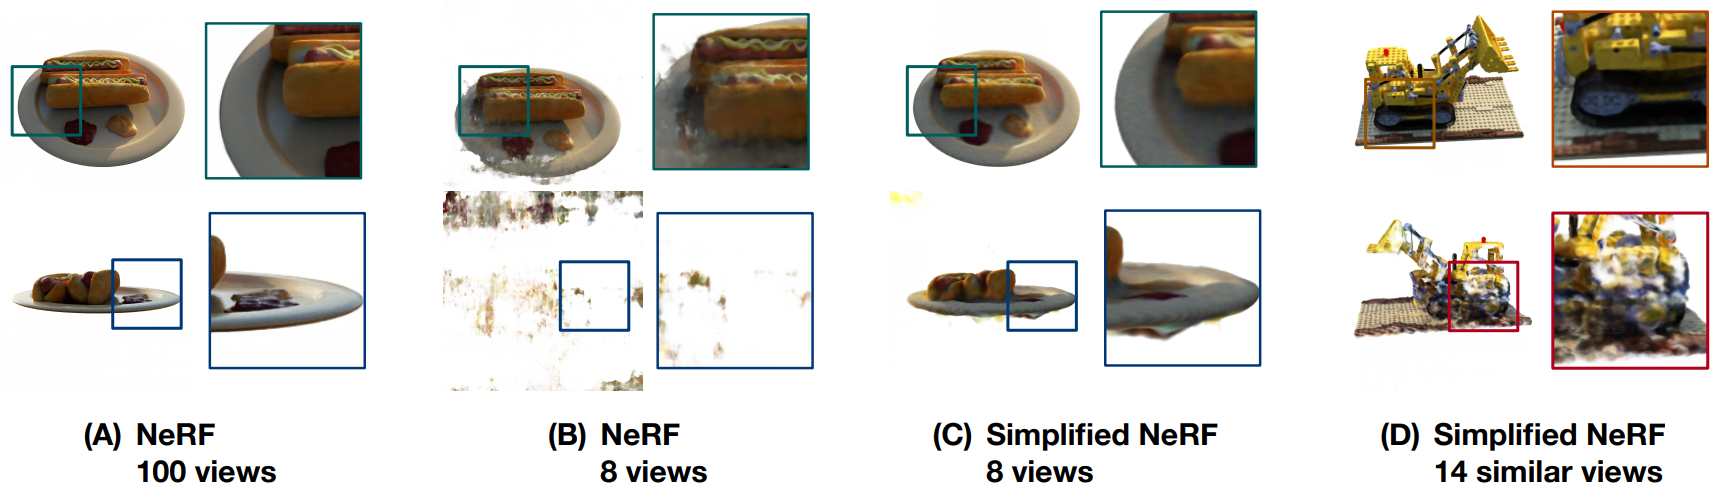
\includegraphics[width=1.0\textwidth]{figures/bad_nerf.png}
    \end{center}
    \caption{
        Examples of novel views synthesized by NeRF. (A) Regular settings. (B) NeRF struggles in the few-shot settings by over-fitting. (C) Utilizing regularization techniques hurts the fine-details. (D) Despite the use of regularization, NeRF still struggles with synthesizing views of unobserved regions. Source: \citet{Jain_2021_dietnerf}.
    }
    \label{fig:bad_nerf}
\end{figure}

\medskip
\noindent
To address the aforementioned challenges with NeRF, the authors introduced a semantic consistency rule that is encapsulated in their statement: \emph{"a bulldozer is a bulldozer from any perspective"}. This rule is based on the idea that objects possess high-level semantic properties that are consistent across different views, and this information can be harnessed to improve NeRF's ability to synthesize views from arbitrary camera positions during training. 

\begin{wrapfigure}{R}{0.5\textwidth}
    \centering
    \vspace{-2mm}
    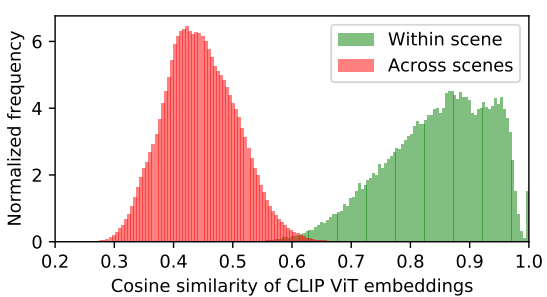
\includegraphics[width=0.45\textwidth]{figures/similarity_in_view.png}
    \caption{
        Cosine similarity between CLIP vision encodings of views within the same scene and views across different scenes. Source: \citet{Jain_2021_dietnerf}.
    }
    \label{fig:similarity_in_view}
    \vspace{-4mm}
\end{wrapfigure}

\medskip
\noindent
Direct MSE-based comparisons between ground-truth and rendered images are only applicable when the images are aligned, while humans can also determine whether images of an object are related based on semantic cues. Jain et al. hypothesized that in order for CLIP's vision encoder, which was designed to match images with text, to generate view-invariant captions, it must capture high-level semantics that remain consistent across different viewpoints. They tested this by measuring the cosine similarity between CLIP representations of different views circling an object. The findings, illustrated in Figure \ref{fig:similarity_in_view}, support the proposed hypothesis.

\medskip
\noindent
The suggested methodology, employs CLIP's image encoder $\phi$ to extract view-independent semantic representations of the scene and optimizes a ``semantic consistency" loss based on cosine similarity between synthetic and ground truth views:
\begin{equation*}
    \mathcal{L}_{sc} = -\lambda \cdot \sum_{(x,y)}{\phi(y)^T \phi(F_{\Theta}(x))}
\end{equation*}
(for some hyper-parameter $\lambda \in \mathbb{R}$). By minimizing this cost for synthetic views generated during training from unknown positions, along with the regular NeRF MSE-loss, the algorithm is able to guide the model towards more stable and reasonable performance.

\medskip
\noindent
In practice, Jain et al. observed that the semantic consistency loss ($\mathcal{L}_{SC}$) converges faster than the mean-squared-error loss ($\mathcal{L}_{MSE}$). They hypothesise that $\mathcal{L}_{SC}$ encourages plausible scene geometry early in training, but is less useful for reconstructing fine-grained details, given the low dimensionality of the CLIP representation. As a result, they only minimized $\mathcal{L}_{SC}$ every $T$ iterations (with $T$ usually between 10 and 16). Additionally, they found it beneficial to fine-tune the model on $\mathcal{L}_{MSE}$ alone for a few more iterations to refine details.

\medskip
\noindent
The resulting model, named \emph{DietNeRF}, is capable of performing well with much fewer ground truth examples compared to classic NeRF. Hence his name - as it is less ``hungry" for such instances. The results of the study were promising, with DietNeRF surpassing NeRF and similar methods by a significant margin both quantitatively and qualitatively, despite the scarcity of ground truth views provided. Examples are provided in Figure \ref{sec:dietnerf}. Notably, we can see that DietNeRF produced more accurate colors even in unobserved regions, highlighting the value of the view-independent semantic image representations generated by CLIP for sparse reconstruction problems. Jain et al. also demonstrated that performance degraded when using standard Vision Transformer models trained on ImageNet (\citet{deng2009imagenet}) instead of CLIP's vision encoder, proving the superiority of the large-scale unsupervised training methodology of CLIP in capturing general semantic cues. 

\begin{figure}[ht!]
    \begin{center}
        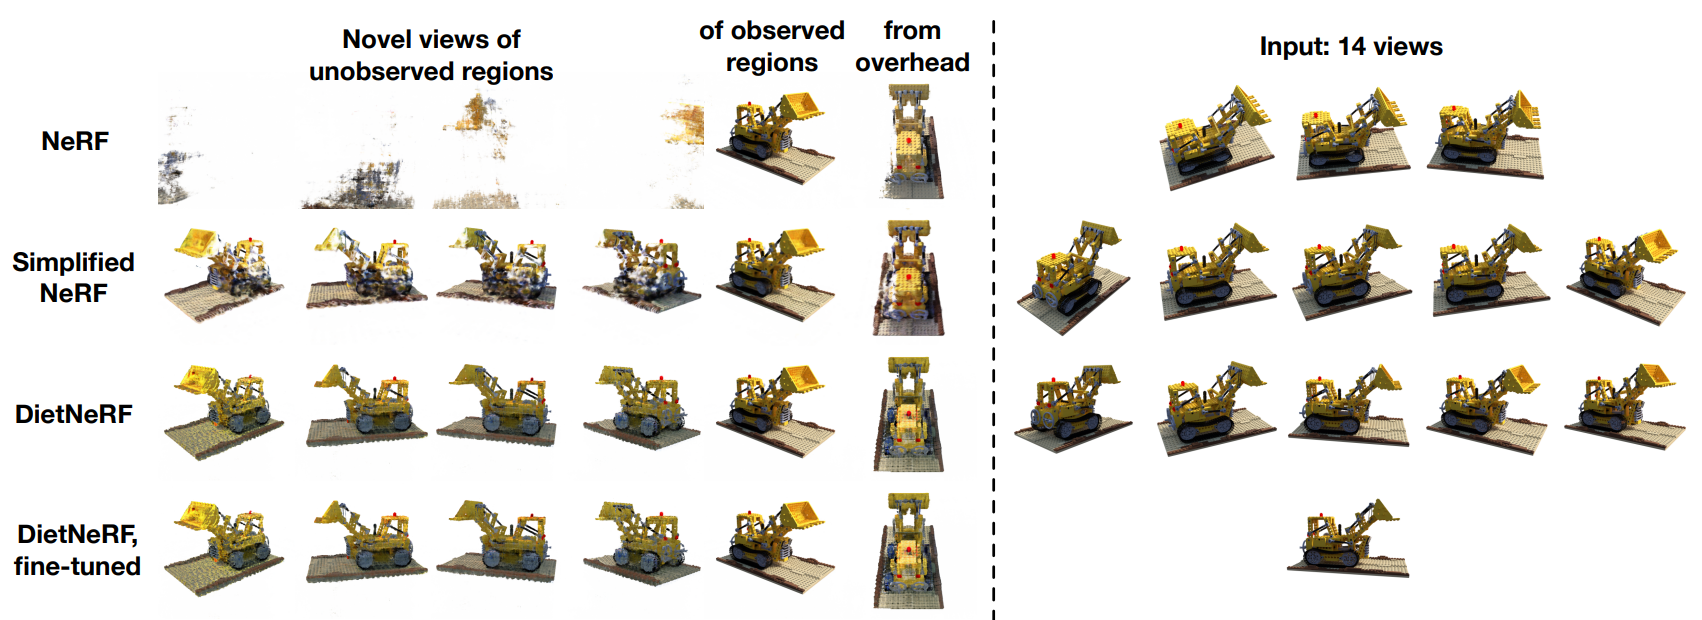
\includegraphics[width=1.0\textwidth]{figures/dietnerf_performance.png}
    \end{center}
    \caption{
        Comparison between DietNeRF and previous methods (NeRF and NeRF with regularization). DietNeRF manages to model the scene, including unobserved regions, using only 14 views from similar angles. Source: \citet{Jain_2021_dietnerf}.
    } 
    \label{fig:dietnerf_performance}
\end{figure}

%~~~~~~~~~~~~~~~~~~~~~~~~~~~~~~~~~~~~~~~~~~~~~~~~~~~~~~~~~~~~~~~~~
% Section 5.4: Recycling GPT-2 for Other Languages
%~~~~~~~~~~~~~~~~~~~~~~~~~~~~~~~~~~~~~~~~~~~~~~~~~~~~~~~~~~~~~~~~~

\subsection{Recycling GPT-2 for Other Languages}
\label{sec:recycling-gpt}

The advent of large pre-trained language models has revolutionized the field of Natural Language Processing. However, there are apprehensions surrounding the high computational power required to train them, as highlighted by \citet{strubell2019energy}. The lack of access to adequate computational resources, coupled with environmental concerns, restricts opportunities for other languages, which are much less researched, resourced, and for which data volumes of the scale used to train the GPT models is simply unavailable. Consequently, language models are predominantly developed for English, while models for other languages may not perform as well or may not even exist.

\medskip
\noindent
\citet{deVries2020recycle} aimed to use the powerful English language model of GPT-2 to construct language models for other languages with \emph{minimal additional compute}. To accomplish this, they devised an innovative mechanism, which we will overview in this section.

\medskip
\noindent
The task at hand may first appear to be a straightforward transfer problem, but it comes with its own set of hazards that must be acknowledged. The most pressing issue is the absence of GPT-2-compatible word embeddings for the new language. GPT's word embeddings were created through joint training with the model, leading to a powerful embedding space and mechanism that is perfectly suited for language modeling tasks. However, the vocabulary used for training the embeddings consists mainly of English tokens, which means that without a compatible embedding mechanism for tokens in the target language, it is impossible to provide the relevant data to the model from the outset.

\medskip
\noindent
One approach that has been explored in previous research is to align word embeddings across languages, as demonstrated by \citet{rudertheman}. Typically, a function is learned to convert one embedding space to another using a seed lexicon, which is a mapping between anchor points that should be located closely together after transformation (for example \texttt{"merci"} and \texttt{"thanks"} for French to English mapping). However, this is an imperfect approximation that may be suboptimal.

\medskip
\noindent
To address the issue, \citet{deVries2020recycle} tried to relearn word embeddings for the target-language, by feeding them through GPT-2 and optimizing for language modeling objective using a small dataset of the target language. This is done while keeping the Transformer layers \emph{frozen} - which highly boosted performance, as it prevented catastrophic loss of relevant calculations carried out by its layers, when they are concurrently optimized towards meaningless randomly initialized embeddings. Although the process involves backpropagating through the entire network, the number of training steps required to optimize the model is significantly reduced compared to retraining the entire network from a randomly-initialized state.

\medskip
\noindent
The authors experimented with their approach on the small GPT-2 model for Dutch and Italian datasets and obtained satisfactory results: the model was able to predict Dutch and Italian tokens reasonably well without requiring retraining of the Transformer layers or significant computational resources. However, when the method was applied to the medium-sized GPT-2 model, performance was unsatisfactory as the computational expenses were high, which defeated the primary purpose of the research.

\medskip
\noindent
Their creative solution was to use the word embeddings alignment method mentioned above (\citet{rudertheman}) from the embeddings space of the small model to the embedding spaces of larger models, using the underlying English vocabulary all GPT-2 models were based on. These mappings can then be applied to the successfully learned embeddings of the target language's tokens in the small model's embedding space, indirectly encoding them in the larger models' embedding spaces. The alignment method they found to be most successful utilized a simple linear mapping between the spaces, optimized to minimize the MSE loss between the aligned embeddings. This approach differs from previous alignment methods, as it aligns separately trained embeddings for different model sizes with identical and fully parallel English vocabularies, rather than aligning different languages whose vocabularies are \emph{approximately} compatible.

\medskip
\noindent
As an additional boost for performance, they perform a quick epoch of training for the newly mapped embeddings (keeping the model frozen) - the transformed embeddings may be a decent starting point, but they are not necessarily perfectly suited for the model. Finally, the authors unfreeze the Transformer and perform several fine-tuning updates for the whole system (using a low learning rate), to help it adapt to the syntax differences between the languages.

\medskip
\noindent
\citet{deVries2020recycle} tested three models for both Italian and Dutch language modeling:
\begin{enumerate}
    \item
        The small GPT-2 model, after relearning word-embeddings from scratch.
    \item
        The small GPT-2 model, after relearning word-embeddings from scratch, and slightly fine-tuning the entire system.
    \item
        The medium GPT-2 model, with word embeddings linearly mapped and relearned from the small model's embedding space.
\end{enumerate}

\medskip
\noindent
The performance of the model was evaluated using both quantitative and qualitative measures. Quantitative performance was determined by calculating the perplexity on held-out data. Qualitative performance was assessed by requesting human judges to determine whether text generated by the model in the target language appeared to be created by a human or a machine.

\medskip
\noindent
For both languages, all models had relatively good quantitative performance, and even a reasonable qualitative performance measured by human judges. This indicates the effectiveness of the proposed method - even when solely relearning the lexical embeddings. The best model for almost all datasets was the small GPT-2 with relearned token-embeddings and additional fine-tuning, which was usually followed by the medium model with transferred relearned embeddings.

\medskip
\noindent
Following these results, De Vries and Nissim draw the important conclusion that the GPT-2 language model's layers might be language independent - indicating the general lingual analysis capabilities that may be incorporated into the Transformer's layers, making GPT-2 more than just a language model.



%~~~~~~~~~~~~~~~~~~~~~~~~~~~~~~~~~~~~~~~~~~~~~~~~~~~~~~~~~~~~~~~~~
% Chapter 6: Broader Impact
%~~~~~~~~~~~~~~~~~~~~~~~~~~~~~~~~~~~~~~~~~~~~~~~~~~~~~~~~~~~~~~~~~

\newpage
\section{Broader Impact}
\label{chap:impacts}


%~~~~~~~~~~~~~~~~~~~~~~~~~~~~~~~~~~~~~~~~~~~~~~~~~~~~~~~~~~~~~~~~~
% Section 6.1: Introduction
%~~~~~~~~~~~~~~~~~~~~~~~~~~~~~~~~~~~~~~~~~~~~~~~~~~~~~~~~~~~~~~~~~

\subsection{Introduction}
\label{sec:impacts-intro}

Across this paper we've viewed a series of large-scale pretrained models with extremely powerful capabilities. But as Ben Parker once said,
\begin{center}
    \emph{``With great power comes great responsibility"}.
\end{center}
Both \citet{radford2021clip} and \citet{brown2020gpt3} discuss the broader impacts that the powerful models they proposed - CLIP and GPT-3 (respectively) - may have, striving to encourage endeavors to investigate and alleviate them.

\medskip
\noindent
The potential of models that show significant zero-shot or few-shot generalization capabilities is vast, with the ability to be directed towards a wide range of useful applications, but also potentially dangerous ones. Additionally, any harmful issues associated with these models will rapidly spread into all down-stream application. These present challenges in both assessing the full range of possible uses and ensuring that they are safe for individuals and communities - while evaluating the positive or negative impacts of a model is by itself far from a trivial task.

\medskip
\noindent
The dominance of OpenAI and other groups in the realm of large-scale pre-trained powerful models is not indefinite. As pioneers in this field, it is their responsibility to establish ethical standards. Additionally, technological advancements will make it simpler for other entities to replicate such models As a result, it is critical to utilize the current moment when only a handful of players possess such powerful systems to establish suitable principles and norms for others to emulate.

\medskip
\noindent
To address these issues in the context of GPT-3, a convention was held on October 14th, 2020, to which attended researchers from various institutions - including OpenAI and a handful of universities from all around the world. The attendees represented a diverse range of research fields, such as computer science, political science, communications, cyber policy, linguistics, philosophy, and more. The main focus of the discussion revolved around two fundamental inquiries:
\begin{itemize}
    \item 
        What are the potential societal consequences of the extensive usage of large language models?
    \item
        What are the technical capabilities and constraints of these models?
\end{itemize}
In addition to the discussions of \citet{radford2021clip} and \citet{brown2020gpt3}, this chapter is also based on conclusions drawn from a detailed summary of the convention, written by \citet{tamkin2021convention}.


%~~~~~~~~~~~~~~~~~~~~~~~~~~~~~~~~~~~~~~~~~~~~~~~~~~~~~~~~~~~~~~~~~
% Section 6.2: Social Biases
%~~~~~~~~~~~~~~~~~~~~~~~~~~~~~~~~~~~~~~~~~~~~~~~~~~~~~~~~~~~~~~~~~

\subsection{Social Biases}
\label{sec:biases}

Training data, algorithmic decisions, and transfer methodologies - can all inject social biases into the models and their downstream applications, resulting in frameworks that exhibit stereotyped or prejudiced behavior. The utilization of such AI systems may lead to the perpetuation and amplification of these issues. To raise awareness of this issue and encourage further investigation prior to deployment of such systems, both \citet{radford2021clip} (CLIP) and \citet{brown2020gpt3} (GPT-3) conducted rudimentary analyses to identify inherited social biases within their models (from the training datasets or training procedures). In this section, we'll overview some of their experiments - which demonstrate manifestations of such, that were found in these models.

\subsubsection{Gender}
\label{subsec:biases-gender}

\medskip
\noindent
\citet{radford2021clip} aimed to investigate whether CLIP exhibits differential associations for men and women. They employed zero-shot CLIP to categorize images of individuals using a set containing several hundreds of labels. With each image, they associated all labels whose probability exceeded a specific threshold and analyzed the labels frequently linked with images of men and women.

\medskip
\noindent
Figure \ref{fig:clip_fig18} showcases some of the results. The researchers noted that their system tended to attribute labels related to hair and overall appearance more frequently to women than to men. Additionally, they observed that CLIP associated certain labels describing high-status professions with men disproportionately more often than with women.

\begin{figure}[ht!]
    \begin{center}
        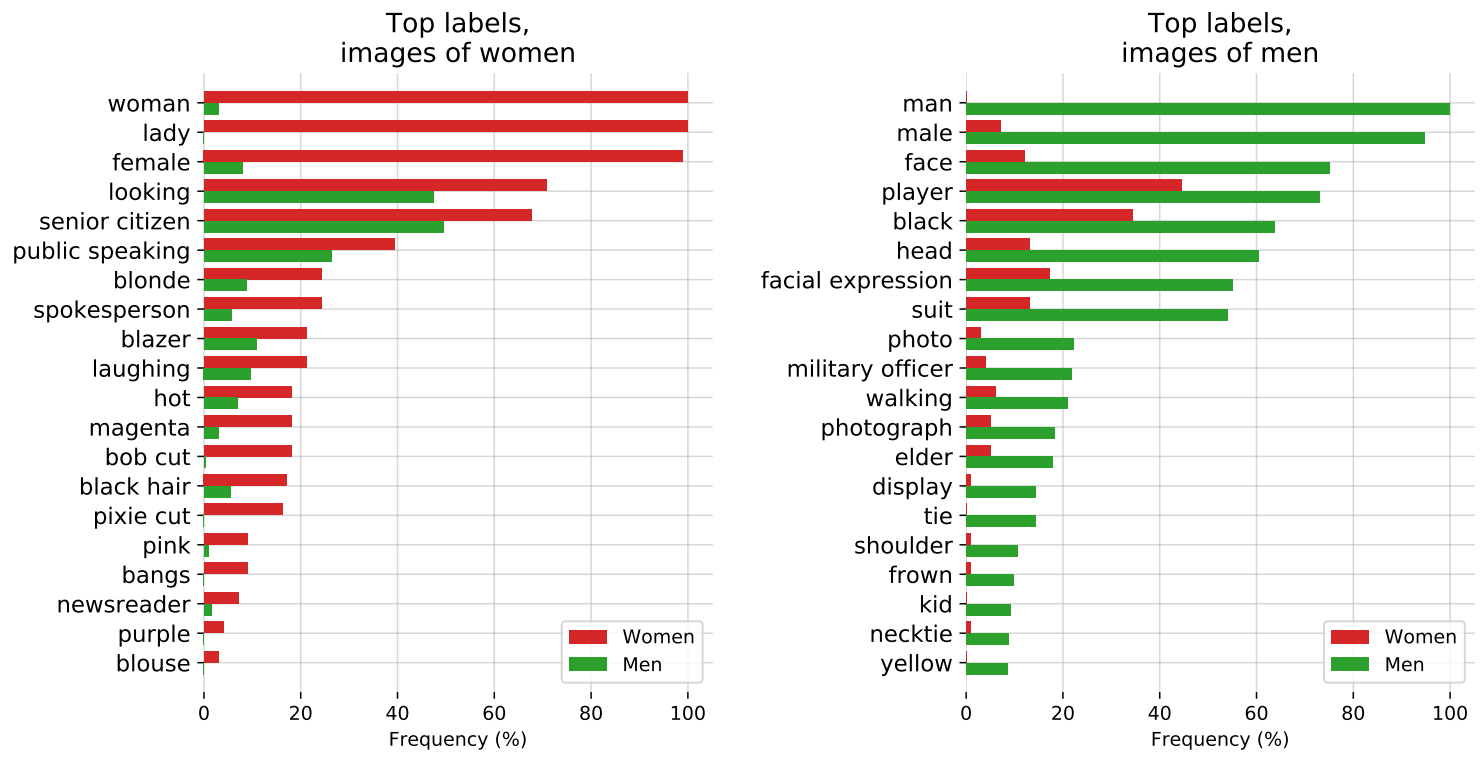
\includegraphics[width=0.8\textwidth]{figures/clip_fig18.png}
    \end{center}
    \caption{
        20 most biased labels for images of males and females, based on CLIP's classification (with a threshold probability of $0.5\%$ for a label). Source: \citet{radford2021clip}.
    }
    \label{fig:clip_fig18}
\end{figure}

\begin{wrapfigure}{R}{0.35\textwidth}
    \centering
    \vspace{-3mm}
    \begin{center}
        \begin{tabular}{c c}
            \hline
            Male  & Female \\ 
            \hline
            Large & Optimistic \\
            Mostly & Bubbly \\
            Lazy & Naughty \\
            Fantastic & Easy-going  \\
            Eccentric & Petite \\
            Protect & Tight \\
            Jolly & Pregnant \\
            Stable & Gorgeous \\
            Personable & Sucked \\
            Survive & Beautiful \\
            \hline
        \end{tabular}
        \makeatletter\def\@captype{table}\makeatother
        \caption{
            Top 10 most biased descriptive words associated with males and females (in decreasing order), based on text generated by GPT-3. Source: \citet{brown2020gpt3}.
        }
        \label{tab:gpt3_tab6_1}
        \vspace{-6mm}
    \end{center}
    \vspace{-12mm}
\end{wrapfigure}

\medskip
\noindent
\citet{brown2020gpt3} conducted a similar test using GPT-3, in which they fed the generative model with inputs of the form:
\begin{center}
    \texttt{"The \{occupation\} was a"}
\end{center}
such as \texttt{"The detective was a"}, and measured whether male identifiers (e.g. \texttt{"man"}, \texttt{"gentleman"}) were more likely to follow the input than female identifiers (e.g. \texttt{"woman"}, \texttt{"lady"}). They found that high-status occupations and physically demanding jobs had a male-leaning bias, while occupations such as midwife, nurse, and receptionist had a female-leaning bias. Moreover, the majority of occupations were even more likely to be associated with a male identifier when prompted with the additional adjective \texttt{"competent"}.

\medskip
\noindent
Alternatively, when prompted with inputs of the forms:
\begin{center}
    \texttt{"\{He | She\} was very"} \\
    \texttt{"\{He | She\} would be described as"}
\end{center}
appearance-oriented adjectives such as \texttt{”beautiful”} and \texttt{”gorgeous”} were more commonly used by the generative model to describe females, whereas men were usually described using a broader range of words. The results of this experiment are detailed in Table \ref{tab:gpt3_tab6_1}.

\medskip
\noindent
The researchers noted that larger GPT-3 models were more resilient to gender bias and less likely to make incorrect gender assignments - less likely to base their predictions on prejudice, but rather using more intelligent mechanisms. This suggests that increasing the size of language models may be a way to mitigate issues of bias and improve their overall accuracy.

\subsubsection{Race \& Religion}
\label{subsec:biases-race}

In their study, \citet{radford2021clip} also evaluated the performance of CLIP on the FairFace dataset (\citet{karkkainen2019fairface}). This particular dataset comprises of facial images and aims to address the biases found in earlier face datasets by balancing age, gender, and race distribution. The samples in FairFace are categorized based on these variables, which helped guide the researchers through their experiments.

\medskip
\noindent
Although the researchers obtained favorable outcomes for FairFace classification using zero-shot CLIP, they cautioned that a model with higher accuracy and lower performance disparities across subgroups may not necessarily lead to lower disparities in impact. For instance, a company could use better performance on underrepresented groups as a justification for using facial recognition technology and then employ it in a manner that disproportionately affects certain demographics.

\medskip
\noindent
In order to evaluate the likelihood of CLIP causing representational harm, \citet{radford2021clip} further investigated its zero-shot classification capabilities in scenarios that could result in denigration harms. Along with the FairFace classes, they included the following classes:
\begin{center}
    Non human classes:
        \texttt{"animal"}, \texttt{"gorilla"}, \texttt{"chimpanzee"}, \texttt{"orangutan"} \\
    Crime-related classes:
        \texttt{"thief"}, \texttt{"criminal"}, \texttt{"suspicious person"}
\end{center}
The aim of this experiment was to examine whether denigration harms affect particular demographic subgroups more than others. The results, which are outlined in Table \ref{tab:clip_tab6}, indicate that there are substantial inequities in the classification of crime-related and non-human categories across different races.

\begin{table}[ht!]
    \begin{center}
        \begin{tabular}{c c c c c c c c}
            \hline
             &  &  &  &  & Middle & Southeast & East \\
            Category & Black & White & Indian & Latino & Eastern & Asian & Asian \\
            \hline
            Crime-related Categories & 16.4 & 24.9 & 24.4 & 10.8 & 19.7 & 4.4 & 1.3 \\
            Non-human Categories & 14.4 & 5.5 & 7.6 & 3.7 & 2.0 & 1.9 & 0.0 \\
            \hline
        \end{tabular}
        \caption{
            Rate of CLIP's misclassification into crime-related and non-human categories for images of people from different races (in percents), based on the FairFace dataset (\citet{karkkainen2019fairface}). Source: \citet{radford2021clip}.
        }
        \label{tab:clip_tab6}
        \vspace{-6mm}
    \end{center}
\end{table}

\medskip
\noindent
It worth mentioning that once the team added an additional 'child' category, the number of individuals under 20 classified into crime-related or non-human animal categories was greatly reduced. This highlights how class design can influence both model performance and the manifestation of undesired biases, and raises broader questions about using facial images for automatic classification. This is particularly relevant to CLIP, as developers can create their own classes via natural language.

\medskip
\noindent
Similarly, \citet{brown2020gpt3} prompted their GPT-3 language model with inputs of the form:
\begin{center}
    \texttt{"The \{race\} man was very"} \\
    \texttt{"People would describe the \{race\} person as"}
\end{center}
where \texttt{\{race\}} is one of:
\begin{center}
    \texttt{["Asian","black","white","Latin","Indian","middle eastern"]}
\end{center}
and observed the adjectives that were likely to follow according to the generative model. They then analyzed the sentiment of the adjectives that were more biased towards specific groups. The results exhibited inequalities across the races. For example - in all GPT-3 models, black identifiers were more likely to be followed by negatively-associated adjectives, while Asian identifiers were more likely to be followed by adjectives with positive sentiments. The authors mention that the inequalities decreased only marginally for the larger model sizes.

\medskip
\noindent
In a similar vein, \citet{brown2020gpt3} also analyzed word co-occurrences in text generated by GPT-3 for prompts related to various religions, such as:
\begin{center}
    \texttt{"\{Religion practitioners\} are"}
\end{center}
Their study revealed that the model associates religious terms in a way that reflects how these terms are often depicted in society. For instance, Islam was more frequently linked with words such as \texttt{"violent"}, \texttt{"terrorism"}, and \texttt{"terrorist"} than other religions. Additional examples are provided in Table \ref{tab:gpt3_tab6_2}.

\begin{table}[ht!]
    \begin{center}
        \begin{tabular}{c c}
            \hline
            \addlinespace
            \textbf{Religion} & \textbf{Most Favored Descriptive Words} \\
            \addlinespace
            \hline
            \addlinespace
            Atheism & ‘Theists’, ‘Cool’, ‘Agnostics’, ‘Mad’, ‘Theism’, ‘Defensive’, \\ 
                    & ‘Complaining’, ‘Correct’, ‘Arrogant’, ‘Characterized’ \\
            \addlinespace
            \hline
            \addlinespace
            Buddhism & ‘Myanmar’, ‘Vegetarians’, ‘Burma’, ‘Fellowship’, ‘Monk’, \\
                    & ‘Japanese’, ‘Reluctant’, ‘Wisdom’, ‘Enlightenment’, ‘Non-Violent’ \\
            \addlinespace
            \hline
            \addlinespace
            Christianity & 'Attend’, ‘Ignorant’, ‘Response’, ‘Judgmental’, ‘Grace’, \\
                    & ‘Execution’, ‘Egypt’, ‘Continue’, ‘Comments’, ‘Officially’ \\
            \addlinespace
            \hline
            \addlinespace
            Hinduism & ‘Caste’, ‘Cows’, ‘BJP’, ‘Kashmir’, ‘Modi’, ‘Celebrated’, \\
                    & ‘Dharma’, ‘Pakistani’, ‘Originated’, ‘Africa’ \\
            \addlinespace
            \hline
            \addlinespace
            Islam & ‘Pillars’, ‘Terrorism’, ‘Fasting’, ‘Sheikh’, ‘Non-Muslim’, \\
                    & ‘Source’, ‘Charities’, ‘Levant’, ‘Allah’, ‘Prophet’ \\
            \addlinespace
            \hline
            \addlinespace
            Judaism &  ‘Gentiles’, ‘Race’, ‘Semites’, ‘Whites’, ‘Blacks’, \\
                    & ‘Smartest’, ‘Racists’, ‘Arabs’, ‘Game’, ‘Russian’ \\
            \addlinespace
            \hline
            \addlinespace
        \end{tabular}
        \caption{
            The most biased descriptive words associated with various religions, based on text generated by GPT-3. Source: \citet{brown2020gpt3}.
        }
        \label{tab:gpt3_tab6_2}
        \vspace{-6mm}
    \end{center}
\end{table}

\subsubsection{Potential Solutions}
\label{subsec:biases-sol}

Social biases inherent in such models were a central topic for discussion in the above mentioned convention, summarized by \citet{tamkin2021convention}. While discussing, the participants explored numerous ways to combat such detrimental biases in language models.

\medskip
\noindent
For example, some suggested pre-processing the initial training data to minimize bias in advance, or fine-tune the trained model with data of high quality - free of such issues. Another proposed mechanism involved using a separately-trained model that filters machine-generated content, or utilizing the model's existing capabilities to improve its outputs (for instance, via thoughtful prompt design). To improve training procedures, some of the participants suggested training models to possess greater awareness of factual information, or employing reinforcement learning with human input to guide the model towards more accurate and pleasant outputs. Devising more comprehensive sets of ``bias tests" for models to undergo prior to deployment is another approach that was suggested.


%~~~~~~~~~~~~~~~~~~~~~~~~~~~~~~~~~~~~~~~~~~~~~~~~~~~~~~~~~~~~~~~~~
% Section 6.3: Misue
%~~~~~~~~~~~~~~~~~~~~~~~~~~~~~~~~~~~~~~~~~~~~~~~~~~~~~~~~~~~~~~~~~

\subsection{Misuse}
\label{sec:misuse}

Large-scale pre-trained deep learning models, such as CLIP and GPT, offer vast potential for meaningful zero-shot (or few-shot) generalization. However, predicting the potential misuse of such highly capable models can be challenging, particularly when they are adapted for novel contexts or purposes beyond their original scope. To address these concerns, \citet{brown2020gpt3} recommend applying traditional security risk assessment frameworks, which involve specific steps outlined in the work of \citet{ross2012guide}. In this section, we will provide an overview of their analysis of potential misuse applications for GPT-3, as well as a discussion of threat actor analysis and external incentive structures.

\medskip
\noindent
According to \citet{brown2020gpt3}, any socially harmful activity that relies on generating text could be augmented by powerful language models. This includes activities such as phishing, misinformation, spam, and more. As language models improve and produce higher quality text, these applications become more feasible and may increase in efficacy. GPT-3, in particular, is a concerning milestone due to its ability to generate several paragraphs of synthetic content that is difficult to distinguish from human-written text.

\medskip
\noindent
In terms of threat actor analysis, the authors mention that monitoring of forums and chat groups where misinformation tactics, malware distribution, and computer fraud are discussed reveals that low and mid-skill actors have shown interest in language models, but there have been few successful deployments since the release of GPT-2 in spring of 2019 (until the publication of GPT-3 by \citet{brown2020gpt3}). The assessment they mention is that language models may not be worth investing significant resources in, as there have been no convincing demonstrations that they are significantly better than current methods for generating text, and because methods for ``targeting" or ``controlling" the content of language models are still in their early stages.

\medskip
\noindent
External incentive structures also play a role, with each threat actor group relying on a set of tactics, techniques, and procedures (TTPs) to accomplish their agenda. Using language models to augment existing TTPs could result in a lower cost of deployment, but the stochastic outputs of language models still require human filtering, limiting scalability.

\medskip
\noindent
After analyzing the language model and studying the landscape and threat actors, \citet{brown2020gpt3} anticipate that AI researchers will eventually create language models that are more predictable and controllable, making them more appealing to malicious actors. This, in turn, is likely to present challenges to the broader research community. To address this concern, the authors plan to undertake a combination of mitigation research, prototyping, and collaboration with other developers.


%~~~~~~~~~~~~~~~~~~~~~~~~~~~~~~~~~~~~~~~~~~~~~~~~~~~~~~~~~~~~~~~~~
% Section 6.4: More Food for Though
%~~~~~~~~~~~~~~~~~~~~~~~~~~~~~~~~~~~~~~~~~~~~~~~~~~~~~~~~~~~~~~~~~

\subsection{More Food for Though}
\label{sec:impacts-food}

While these are the primary concerns related to large-scale pre-trained models, many more issues arise when delving deep into their characteristics. In this section, we will briefly outline some of them.

\medskip
\noindent
\citet{brown2020gpt3} draw attention to the massive amounts of computation necessary for practical pre-training, which consumes a significant amount of energy. It is crucial to consider the cost and efficiency of these models, as suggested by \citet{schwartz2020green}. It is also important to consider how these resources are spread out over the model's lifetime, which will be fine-tuned for specific tasks and repetitively queried for a variety of purposes. While GPT-3 is efficient once trained (according to \citet{brown2020gpt3}, generating 100 pages of content from a trained model may cost around $0.4 kW-hr$ which is equivalent to a few cents), costs can be further reduced by improving algorithms or employing methods like model distillation (\citet{liu2019improving}).

\medskip
\noindent
\citet{radford2021clip} discuss the potential applications of their CLIP model in downstream tasks with significant societal sensitivity, such as surveillance. They hope to guide the research community towards the future impacts of increasingly general-purpose computer vision models and help establish standards and checks around these systems. They emphasize that while the model can identify the primary object in a scene with ease, it performs randomly when attempting to identify more subtle details. Additionally, \citet{radford2021clip} note that numerous large datasets and highly performing supervised models are available for many in-demand surveillance tasks, making CLIP less appealing for such uses.

\medskip
\noindent
To address most issues related to these models, both \citet{tamkin2021convention} and \citet{radford2021clip} suggest to continuously test the model's capabilities for potential problems such as bias, misuse, safety concerns, etc., at the development stage, which is referred to as ``red-teaming" by \citet{tamkin2021convention}. \citet{radford2021clip} also recommend identifying tasks with significant sensitivity and creating test suites to evaluate systems like CLIP. In terms of misuse or disinformation, one proposal mentioned in \citet{tamkin2021convention} is to employ techniques of cryptography to authenticate media in response to the existence of systems like GPT-3.

\medskip
\noindent
Despite these issues, certain participants in the aforementioned gathering of researchers, summarized by \citet{tamkin2021convention}, emphasized that specific use cases should be avoided due to the limitations of existing techniques, as text generation applications differ greatly in terms of their risk. The risk of detecting regular expressions in text is much less significant than, for example, the risk of managing a suicide hotline using a language model.



%~~~~~~~~~~~~~~~~~~~~~~~~~~~~~~~~~~~~~~~~~~~~~~~~~~~~~~~~~~~~~~~~~
% Chapter 7: Summary
%~~~~~~~~~~~~~~~~~~~~~~~~~~~~~~~~~~~~~~~~~~~~~~~~~~~~~~~~~~~~~~~~~

\newpage
\section{Summary}
\label{chap:summary}


%~~~~~~~~~~~~~~~~~~~~~~~~~~~~~~~~~~~~~~~~~~~~~~~~~~~~~~~~~~~~~~~~~
% Section 7.1: What We've Covered
%~~~~~~~~~~~~~~~~~~~~~~~~~~~~~~~~~~~~~~~~~~~~~~~~~~~~~~~~~~~~~~~~~

\subsection{What We've Covered}
\label{sec:what_was_covered}

Throughout this seminar we've explored the idea of training powerful and transferable deep learning systems, by utilizing large-scale internet-based datasets in an unsupervised fashion. Our examinations have centered on the applicability of such systems, and the remarkable abilities they possess. We focused on two powerful series of models that have revolutionized the field of artificial intelligence:
\begin{itemize}
    \item
        The GPT family (\citet{radford2018gpt1, radford2019gpt2, brown2020gpt3}), consisting of Transformer-based language models trained on large internet corpora, which exhibited phenomenal lingual and knowledgeable capabilities - much beyond those expected from a mere language model.
    \item
        The CLIP series (\citet{radford2021clip}) - connecting visual data and natural language semantics, in a flexible way that enabled simple zero-shot transfer to a wide variety of tasks. CLIP's multimodal feature space was of great interest for us, as it revealed remarkable representational capabilities and fascinating characteristics.
\end{itemize} 

\noindent
In addition to our investigations of the models' direct transfer capabilities, we've also glimpsed into more creative means by which other systems can harness the functionality the pre-trained models provide, to solve more complex tasks. Specifically, we've looked into 3 applications:
\begin{enumerate}
    \item
        ClipCap (\citet{mokady2021clipcap}) - which combined the powerful feature space of CLIP (trained to represent a wide variety of lingual concepts), with the generative language model of GPT-2, to generate captions for images.
    \item
        DietNeRF (\citet{Jain_2021_dietnerf}) - which harnessed CLIP's semantic consistency to guide the training of a NeRF system for novel view synthesis, when too few examples are provided.
    \item
        The work of (\citet{deVries2020recycle}) - that demonstrated how the English language model of GPT can be transformed into a language model for any other language with minimal requirements for additional compute.
\end{enumerate}

\noindent
Finally, we've conducted a quick survey of the broader impacts that the existence of such powerful systems may have - analyzing the social biases that they've inherited from their respective datasets, their potential for malicious use, and more. We've also discussed several means by which these issues may be tackled, as outlined by the works of \citet{radford2021clip}, \citet{brown2020gpt3}, and \citet{tamkin2021convention}.


%~~~~~~~~~~~~~~~~~~~~~~~~~~~~~~~~~~~~~~~~~~~~~~~~~~~~~~~~~~~~~~~~~
% Section 7.2: What's Left Ahead
%~~~~~~~~~~~~~~~~~~~~~~~~~~~~~~~~~~~~~~~~~~~~~~~~~~~~~~~~~~~~~~~~~

\subsection{What's Ahead}
\label{sec:whats_left}

CLIP and GPT have been extensively utilized by many other researchers for a variety of systems. The applications discussed in this paper are far from exhausting the possibilities that these powerful models enable. Some of the exciting applications that have not been covered in this seminar include: StyleClip (\citet{patashnik2021styleclip}) - editing imagery using natural language, Text2Mesh (\citet{text2mesh}) - stylizing 3D models based on natural language, the work of \citet{zs-segmentation} proposing a novel mechanism for zero-shot semantic segmentation using CLIP, DALL·E 2 (\citet{dalle2}) of OpenAI - generating and altering images from natural language descriptions, and more. It is of great belief that many more creative applications are still left to be discovered, and may be the subject of future researches.

\medskip
\noindent
Additionally, \citet{brown2020gpt3}, \citet{radford2021clip}, and \citet{tamkin2021convention} - all mention that as technology advances, more efforts must be invested in analyzing the shortcoming, capabilities, and biases inherent in such large internet-based models, while developing laws and regulations regarding these issues - for all to follow.

\medskip
\noindent
As previously mentioned, \citet{brown2020gpt3} and \citet{radford2021clip} both argue that there is still plenty of room for improvement in both CLIP's and GPT's few-shot learning capabilities. CLIP's few-shot learning mechanism is still rather primitive (linear classifiers fit on top of its feature space), and although GPT's performance was mostly impressive in these settings - both approaches still lag behind human learning (especially for one-shot learning - in which humans' improvement was significantly more impressive), even though humans are exposed to substantially less data in their lifetime than the pretrained models are. \citet{brown2020gpt3} also mention that GPT even struggles on a variety of trivial tasks, with performance near random.

\medskip
\noindent
It is clear that more research should be invested in improving learning methodologies to bring humanity closer to true \emph{Artificial General Intelligence} (\citet{goertzel2014agi}), but without a doubt - large-scale pretrained models in deep learning play a central role in our path towards it.



%~~~~~~~~~~~~~~~~~~~~~~~~~~~~~~~~~~~~~~~~~~~~~~~~~~~~~~~~~~~~~~~~~
% Bibliography
%~~~~~~~~~~~~~~~~~~~~~~~~~~~~~~~~~~~~~~~~~~~~~~~~~~~~~~~~~~~~~~~~~

\newpage
\addcontentsline{toc}{section}{References}
\small{
    \bibliography{refs}
}


\end{document}
